
\documentclass[a4paper, 8pt]{extarticle}
\usepackage[utf8]{inputenc}

\title{Program Analysis for System Security and Reliability FS20}
\author{jasonf & joels }
\date{March 2020}

\usepackage{natbib}
\usepackage{graphicx}
\usepackage{amssymb}
\usepackage{fourier}
\usepackage{array}
\usepackage{svg}
\usepackage{amsmath}
\usepackage{xcolor}
%\usepackage[parfill]{parskip}
\newcommand{\myparagraph}[1]{\paragraph{#1}\mbox{}\\}
\usepackage{adjustbox}

% Multi-column layout
\usepackage{multicol}

%Figures folder
\graphicspath{{Figures/}}

% Manually set page marginshttps://de.overleaf.com/project/5e791732b70cd40001ef8300
\usepackage[margin=0.5cm]{geometry}

% Manually set margins on lists
\usepackage{enumitem}
% Change list margins - https://tex.stackexchange.com/questions/10684/vertical-space-in-lists
\setlist{leftmargin=3mm, nosep}
% or \setlist{noitemsep} to leave space around whole list

\definecolor{orange}{rgb}{1,0.5,0}
\definecolor{green}{rgb}{0.0, 0.5, 0.0}

\begin{document}
\begin{multicols*}{2}
\maketitle
\tableofcontents
\section{Blockchain Basics and Bitcoin}
\subsection{Hash Functions}
\paragraph{Properties:}
\begin{itemize}
    \item Arbitrary input size
    \item Fixed-output size
    \item Deterministic (equal inputs hash to the same value)
    \item Uniform (inputs are mapped evenly to the space of possible outputs)
    \item Efficient (should be fast to compute)
\end{itemize}
\textbf{Note:} Collisions always exists since input space is unbounded. However, cryptographic hash functions ensure collisions are hard to find
\paragraph{Cryptographic hash functions properties:}
\begin{itemize}
    \item \textbf{Pre-image resistant: }Given $y \in Y,$ it is infeasible to find $x \in X$ such that $h(x)=y$
    \item \textbf{Second pre-image resistant: }Given $x \in X,$ it is infeasible to find $x^{\prime} \in X$ such that $x \neq x^{\prime}$ and $h(x)=h\left(x^{\prime}\right)$
    \item \textbf{Collision resistance: }It is infeasible to find a pair $\left(x, x^{\prime}\right) \in X \times X$ such that $x \neq x^{\prime}$ and $h(x)=$ $h\left(x^{\prime}\right)$. This implies second-pre-image resistance
\end{itemize}
\paragraph{Applications: }
\begin{itemize}
    \item \textbf{Data equality: } If we know that $h(x)=h(y)$ and $h$ is a cryptographic hash function, then it is safe to assume that $x=y$
    \item \textbf{Data integrity: } 
    \begin{itemize}
        \item To verify the integrity a piece of data $\color{blue}d$, we can remember its hash, $\texttt{\textcolor{blue}{hash}}$ = $\textcolor{blue}{h}(d)$
        \item Later, when we obtain $\color{red}d^{\prime}$ from $\texttt{\textcolor{red}{untrusted source}}$, we can verify whether $\texttt{\textcolor{blue}{hash}}$ = $\color{red}h\left(d^{\prime}\right)$ to check whether $\color{blue}d$ = $\color{red}d^{\prime}$
        \item Useful because \texttt{\textcolor{blue}{hash}} is small (e.g. 256 bits)
    \end{itemize}{}
\end{itemize}{}
\paragraph{Crypto puzzles: }
\begin{itemize}
    \item \textbf{Puzzle-friendly} For any output $\color{blue}y$, if $\color{red}r$ is chosen from a probability distribution with high min-entropy, then it is infeasible to find $\color{green}x$ such that $h(\texttt{\textcolor{red}{r}} | \texttt{\textcolor{green}{x}})=\texttt{\textcolor{blue}{y}}$
    \item \textbf{Search puzzle:} Given a puzzle ID $\color{blue}id,$ chosen from a probability distribution with high min-entropy (min-entropy = minimum amount of randomness in a distribution or how good it is "shuffled"), and an output target $\color{blue}T \subseteq Y$, find a solution $\color{green}x$ such that $h(\texttt{\textcolor{blue}{id}} | \texttt{\textcolor{green}{x}}) \in \texttt{\textcolor{blue}{T}}$. Puzzle-friendliness implies that no solving strategy is much better than trying random values of $\color{green}x$
\end{itemize}{}
\subsection{Merkle Trees}
\begin{minipage}{.5\linewidth}
    \centering      
    \def\svgwidth{\columnwidth}
    %% Creator: Inkscape inkscape 0.92.4, www.inkscape.org
%% PDF/EPS/PS + LaTeX output extension by Johan Engelen, 2010
%% Accompanies image file 'L2_merkle_trees.pdf' (pdf, eps, ps)
%%
%% To include the image in your LaTeX document, write
%%   \input{<filename>.pdf_tex}
%%  instead of
%%   \includegraphics{<filename>.pdf}
%% To scale the image, write
%%   \def\svgwidth{<desired width>}
%%   \input{<filename>.pdf_tex}
%%  instead of
%%   \includegraphics[width=<desired width>]{<filename>.pdf}
%%
%% Images with a different path to the parent latex file can
%% be accessed with the `import' package (which may need to be
%% installed) using
%%   \usepackage{import}
%% in the preamble, and then including the image with
%%   \import{<path to file>}{<filename>.pdf_tex}
%% Alternatively, one can specify
%%   \graphicspath{{<path to file>/}}
%% 
%% For more information, please see info/svg-inkscape on CTAN:
%%   http://tug.ctan.org/tex-archive/info/svg-inkscape
%%
\begingroup%
  \makeatletter%
  \providecommand\color[2][]{%
    \errmessage{(Inkscape) Color is used for the text in Inkscape, but the package 'color.sty' is not loaded}%
    \renewcommand\color[2][]{}%
  }%
  \providecommand\transparent[1]{%
    \errmessage{(Inkscape) Transparency is used (non-zero) for the text in Inkscape, but the package 'transparent.sty' is not loaded}%
    \renewcommand\transparent[1]{}%
  }%
  \providecommand\rotatebox[2]{#2}%
  \newcommand*\fsize{\dimexpr\f@size pt\relax}%
  \newcommand*\lineheight[1]{\fontsize{\fsize}{#1\fsize}\selectfont}%
  \ifx\svgwidth\undefined%
    \setlength{\unitlength}{720bp}%
    \ifx\svgscale\undefined%
      \relax%
    \else%
      \setlength{\unitlength}{\unitlength * \real{\svgscale}}%
    \fi%
  \else%
    \setlength{\unitlength}{\svgwidth}%
  \fi%
  \global\let\svgwidth\undefined%
  \global\let\svgscale\undefined%
  \makeatother%
  \begin{picture}(1,0.75)%
    \lineheight{1}%
    \setlength\tabcolsep{0pt}%
    \put(0,0){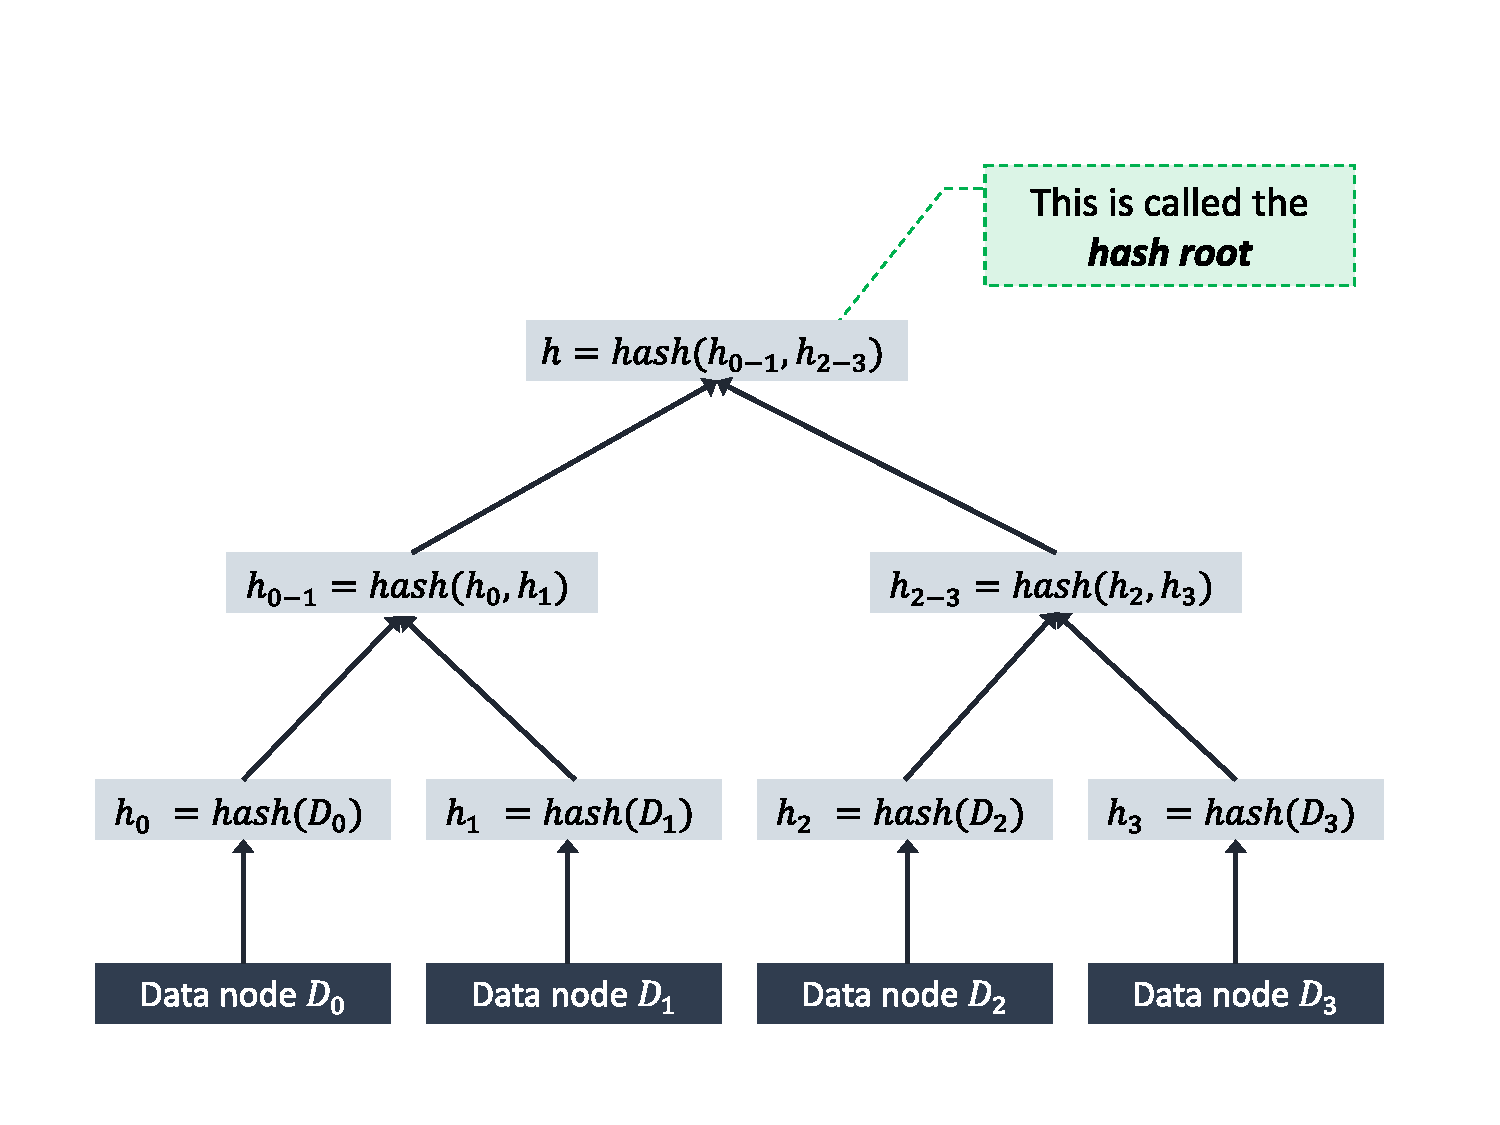
\includegraphics[width=\unitlength,page=1]{Figures/L2_merkle_trees.pdf}}%
  \end{picture}%
\endgroup%
    
\end{minipage}
\begin{minipage}{.5\linewidth}
    \centering      
    \def\svgwidth{\columnwidth}
    %% Creator: Inkscape inkscape 0.92.4, www.inkscape.org
%% PDF/EPS/PS + LaTeX output extension by Johan Engelen, 2010
%% Accompanies image file 'L2_merkle_trees_verification.pdf' (pdf, eps, ps)
%%
%% To include the image in your LaTeX document, write
%%   \input{<filename>.pdf_tex}
%%  instead of
%%   \includegraphics{<filename>.pdf}
%% To scale the image, write
%%   \def\svgwidth{<desired width>}
%%   \input{<filename>.pdf_tex}
%%  instead of
%%   \includegraphics[width=<desired width>]{<filename>.pdf}
%%
%% Images with a different path to the parent latex file can
%% be accessed with the `import' package (which may need to be
%% installed) using
%%   \usepackage{import}
%% in the preamble, and then including the image with
%%   \import{<path to file>}{<filename>.pdf_tex}
%% Alternatively, one can specify
%%   \graphicspath{{<path to file>/}}
%% 
%% For more information, please see info/svg-inkscape on CTAN:
%%   http://tug.ctan.org/tex-archive/info/svg-inkscape
%%
\begingroup%
  \makeatletter%
  \providecommand\color[2][]{%
    \errmessage{(Inkscape) Color is used for the text in Inkscape, but the package 'color.sty' is not loaded}%
    \renewcommand\color[2][]{}%
  }%
  \providecommand\transparent[1]{%
    \errmessage{(Inkscape) Transparency is used (non-zero) for the text in Inkscape, but the package 'transparent.sty' is not loaded}%
    \renewcommand\transparent[1]{}%
  }%
  \providecommand\rotatebox[2]{#2}%
  \newcommand*\fsize{\dimexpr\f@size pt\relax}%
  \newcommand*\lineheight[1]{\fontsize{\fsize}{#1\fsize}\selectfont}%
  \ifx\svgwidth\undefined%
    \setlength{\unitlength}{720bp}%
    \ifx\svgscale\undefined%
      \relax%
    \else%
      \setlength{\unitlength}{\unitlength * \real{\svgscale}}%
    \fi%
  \else%
    \setlength{\unitlength}{\svgwidth}%
  \fi%
  \global\let\svgwidth\undefined%
  \global\let\svgscale\undefined%
  \makeatother%
  \begin{picture}(1,0.75)%
    \lineheight{1}%
    \setlength\tabcolsep{0pt}%
    \put(0,0){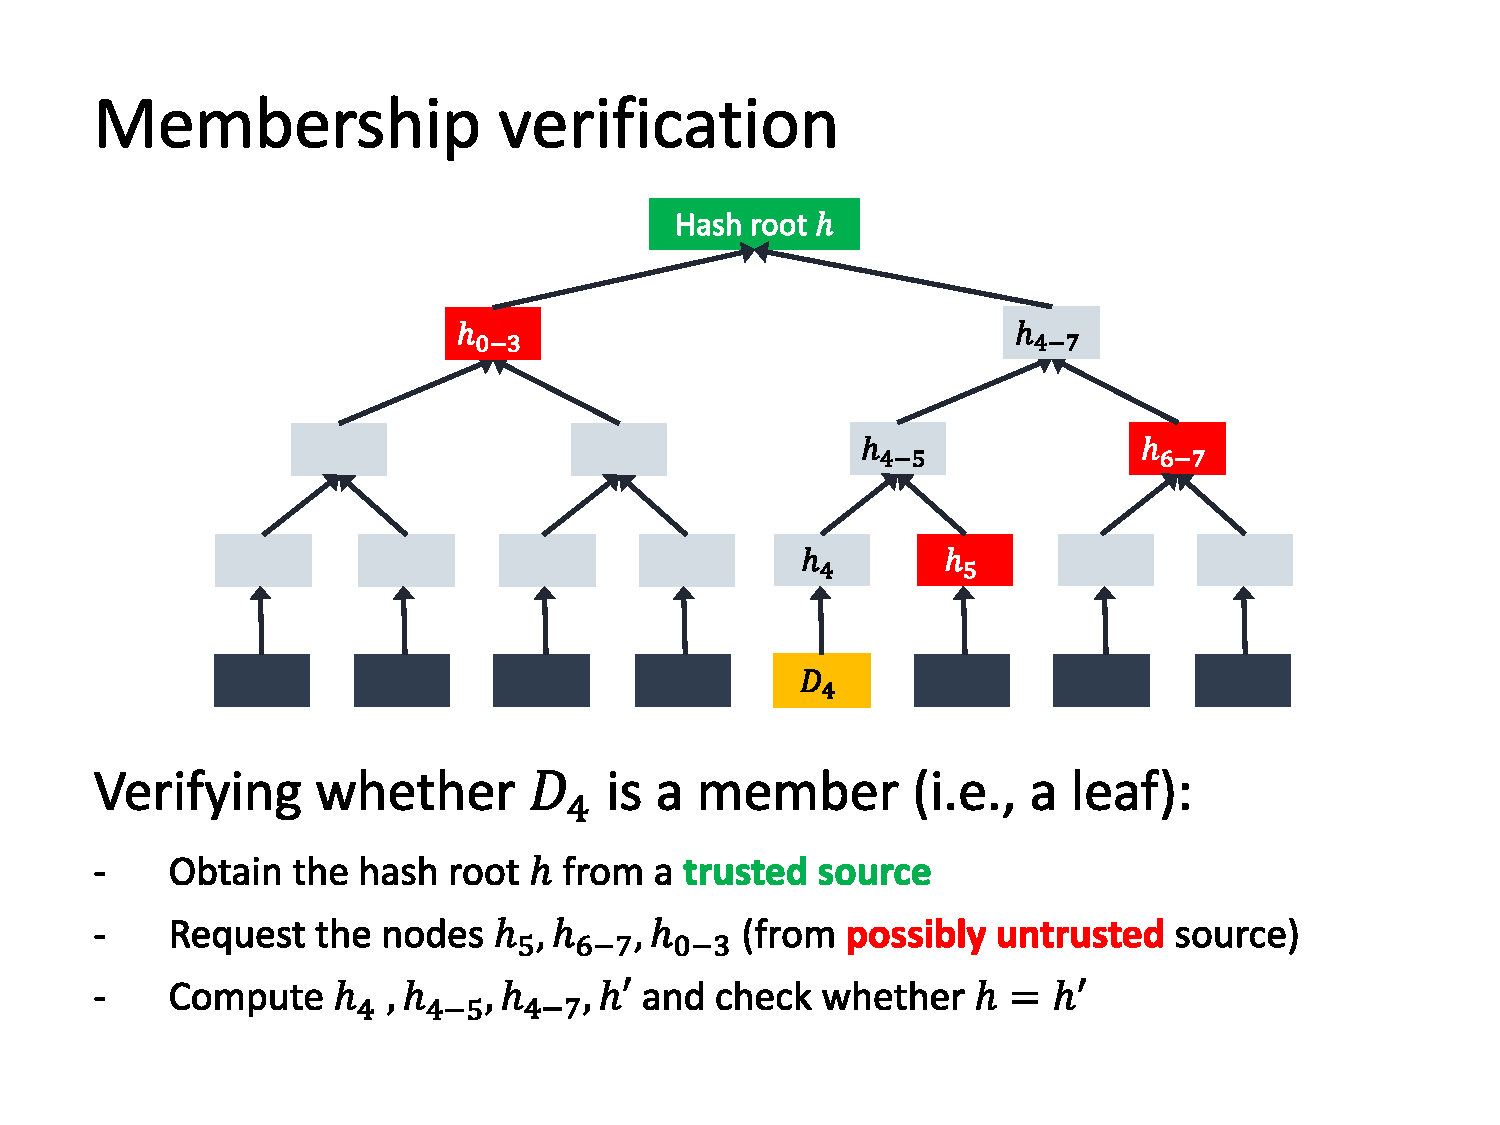
\includegraphics[width=\unitlength,page=1]{Figures/L2_merkle_trees_verification.pdf}}%
  \end{picture}%
\endgroup%
    
\end{minipage}
Membership verification requires $\color{blue}\log (n)$ elements. Useful when the set of data elements is large
\subsection{Digital Signatures}
\textbf{High-level goal: } allow only one user to sign but anyone to verify the signature\newline
\textbf{API for signatures: }
\begin{itemize}
    \item $(\textcolor{red}{sk}, \textcolor{green}{pk})=\texttt{\textcolor{blue}{generateKeys}}(keySize)$
        \begin{itemize}
            \item $\color{red}sk$ is the  $\texttt{\textcolor{red}{secret key}}$, which the owner keeps in private
            \item $\color{green}pk$ is the $\texttt{\textcolor{green}{public key}}$, which is distributed to all users
        \end{itemize}{} 
\item$\textcolor{orange}{sig}$ = $\texttt{\textcolor{blue}{sign}}(\textcolor{red}{sk}, msg)$
\item $\texttt{\textcolor{blue}{verify}}(\textcolor{green}{pk}, msg,\textcolor{orange}{sig})$
\end{itemize}{}
\paragraph{Establish Identity: }
\begin{itemize}
    \item User generates $(\texttt{\textcolor{red}{sk}}, \texttt{\textcolor{green}{pk}})$ key pair
    \item $\texttt{\textcolor{blue}{hash}}(\textcolor{green}{pk})$ is the public name of the user
    \item $\color{red}sk$ allows the user to endorse a statements $stmt$ using a digital signature
    \item $\color{orange}sig$ = $\texttt{\textcolor{blue}{sign}}(\textcolor{red}{sk}, stmt)$
    \item anyone can verify statements endorsed by the user using $\texttt{\textcolor{blue}{verify}}(\textcolor{green}{pk}, \text {stmt}, \textcolor{orange}{sig})$
\end{itemize}
\subsection{Bitcoin Basics}
\paragraph{Distributed Consensus: }
\begin{itemize}
    \item \textbf{Termination: } Every correct process decides on some value
    \item \textbf{Agreement: }  All correct processes decide on the same value
    \item \textbf{Validity: }  If all correct processes propose the same value, then any correct process must decide on that value
\end{itemize}
Traditional motivation: reliability in distributed systems (node replication)
\paragraph{Distributed ledger via consensus: }
\begin{itemize}
    \item To make a transaction, users broadcast transactions to the network nodes
    \item All nodes have a sequence of all blocks of agreed transactions they have reached consensus on
    \item Each node has a set of outstanding transactions (to be added to a block in the blockchain)
\end{itemize}
\textbf{Problems: }
\begin{itemize}
    \item Nodes may crash 
    \item Nodes may be malicious
    \item Network is imperfect
    \begin{itemize}
        \item Not all pair of nodes are connected
        \item Messages may have arbitrary delays
        \item No global time
        \item Nodes may fail 
    \end{itemize}{}
\end{itemize}
\paragraph{Simplified Bitcoin consensus protocol: }
\begin{enumerate}
    \item New transactions are broadcast to all nodes
    \item Each node collects new transactions into a block
    \item In each round, a \texttt{\textcolor{green}{random node}} gets to broadcast its block
    \item Other nodes accept the block only if all transactions in it are valid (unspent, valid signatures)
    \item Nodes express their acceptance of the block by including its hash in the next block they create
\end{enumerate}{}
\textbf{Note: }  \texttt{\textcolor{green}{random node}} selection: 
Select nodes in proportion to a resource that no one can monopolize. Several schemes:
\begin{itemize}
    \item In proportion to computing power: \textcolor{blue}{proof-of-work} used by Bitcoin
    \item In proportion to ownership: \textcolor{blue}{proof-of-stake}
    \item others
\end{itemize}{}
\paragraph{Proof of work:\newline}
\begin{minipage}{0.75\linewidth}
    \def\svgwidth{\columnwidth}
    %% Creator: Inkscape inkscape 0.92.4, www.inkscape.org
%% PDF/EPS/PS + LaTeX output extension by Johan Engelen, 2010
%% Accompanies image file 'L2_PoW.pdf' (pdf, eps, ps)
%%
%% To include the image in your LaTeX document, write
%%   \input{<filename>.pdf_tex}
%%  instead of
%%   \includegraphics{<filename>.pdf}
%% To scale the image, write
%%   \def\svgwidth{<desired width>}
%%   \input{<filename>.pdf_tex}
%%  instead of
%%   \includegraphics[width=<desired width>]{<filename>.pdf}
%%
%% Images with a different path to the parent latex file can
%% be accessed with the `import' package (which may need to be
%% installed) using
%%   \usepackage{import}
%% in the preamble, and then including the image with
%%   \import{<path to file>}{<filename>.pdf_tex}
%% Alternatively, one can specify
%%   \graphicspath{{<path to file>/}}
%% 
%% For more information, please see info/svg-inkscape on CTAN:
%%   http://tug.ctan.org/tex-archive/info/svg-inkscape
%%
\begingroup%
  \makeatletter%
  \providecommand\color[2][]{%
    \errmessage{(Inkscape) Color is used for the text in Inkscape, but the package 'color.sty' is not loaded}%
    \renewcommand\color[2][]{}%
  }%
  \providecommand\transparent[1]{%
    \errmessage{(Inkscape) Transparency is used (non-zero) for the text in Inkscape, but the package 'transparent.sty' is not loaded}%
    \renewcommand\transparent[1]{}%
  }%
  \providecommand\rotatebox[2]{#2}%
  \newcommand*\fsize{\dimexpr\f@size pt\relax}%
  \newcommand*\lineheight[1]{\fontsize{\fsize}{#1\fsize}\selectfont}%
  \ifx\svgwidth\undefined%
    \setlength{\unitlength}{440.89280977bp}%
    \ifx\svgscale\undefined%
      \relax%
    \else%
      \setlength{\unitlength}{\unitlength * \real{\svgscale}}%
    \fi%
  \else%
    \setlength{\unitlength}{\svgwidth}%
  \fi%
  \global\let\svgwidth\undefined%
  \global\let\svgscale\undefined%
  \makeatother%
  \begin{picture}(1,0.43499397)%
    \lineheight{1}%
    \setlength\tabcolsep{0pt}%
    \put(0,0){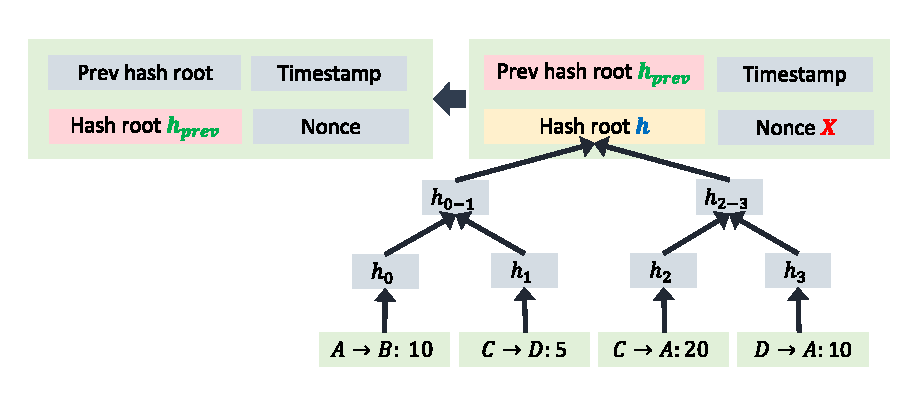
\includegraphics[width=\unitlength,page=1]{Figures/L2_PoW.pdf}}%
  \end{picture}%
\endgroup%
    
\end{minipage}\\
\begin{description}
    \item Given:
        \begin{itemize}
        \item Previous block with hash root $\color{green}h_{\text {prev}}$
        \item Merkle tree consisting of all new transactions with root $\textcolor{blue}h$
        \end{itemize}{}
    \item Find:
        \begin{itemize}
        \item Find a nonce $\texttt{\textcolor{red}{X}}$ such that
        $$
        \operatorname{hash}\left(\textcolor{green}{h_{\text {prev}}}|\textcolor{blue}h|\texttt{\textcolor{red}{X}}\right) \leq \text { difficulty }
        $$
        \end{itemize}{}
\end{description}{}
\paragraph{Properties: }
\begin{itemize}
    \item Difficult to compute
    \begin{itemize}
        \item Current rate in Bitcoin: about 10.2 minutes per block
        \item Probability that a minor succeeds: 10.2 min / fraction of hash power Current hash power: $103,559,611,798 \mathrm{GH} / \mathrm{s}$
    \end{itemize}
    \item Parameterizable cost
    \begin{itemize}
        \item Nodes can adjust the target difficulty
        \item Current difficulty: 15,546,745,765,529
    \end{itemize}{}
    \item Easy to verify
     \begin{itemize}
        \item Other nodes verify that $\operatorname{hash}\left(\textcolor{green}{h_{\text {prev}}}|\textcolor{blue}h|\texttt{\textcolor{red}{X}}\right) \leq \text { difficulty }$

    \end{itemize}{}
    \item Key security assumption
     \begin{itemize}
        \item Attacks infeasible if majority of miners weighted by hash power follow the protocol
    \end{itemize}{}
\end{itemize}{}
\textbf{Note to double spending: } Honest nodes extend the longest valid branch
\paragraph{Incentivizing honest nodes to extend the longest chain}
\begin{itemize}
    \item \textbf{Block reward}. The creator of a block can:
    \begin{itemize}
        \item Include special coin creation transaction in the block 
        \item Choose recipient address of this transaction
        \item Value of transaction is fixed, gets halfed every 210,000 blocks
        \item Block creator ”receives” the reward only if the block ends up on the long-term consensus branch
    \end{itemize}{}
    \item \textbf{Transaction fees}
    \begin{itemize}
        \item Creator of transaction may choose to make output value less than input value. \texttt{\textcolor{blue}{Transaction fee}} = $\sum i n p u t s-\sum o u t p u t s$
    \end{itemize}{}
\end{itemize}{}
\subsection{Bitcoin Scripting:}
\begin{itemize}
    \item \textbf{Data}
    \begin{itemize}
        \item public keys
        \item signatures
    \end{itemize}{}
    \item \textbf{Script opcodes}
    \begin{description}[font=\normalfont,labelwidth=7em,leftmargin =\dimexpr\labelwidth+\labelsep\relax]
        \item [Constants:]  OP\_0, OP\_PUSHDATA\_1, OP\_TRUE
        \item [Flow control:]OP\_IF, OP\_ELSE, ...
        \item [Stack:] OP\_DUP, OP\_SWAP
        \item [Arithmetic:] OP\_ADD, OP\_NEGATE, OP\_LESSTHAN, ...
        \item [Crypto:] OP\_HASH160, OP\_CHECKSIG
        \item [Time:] OP\_CHECKLOCKTIMEVERIFY
    \end{description}{}
    \item \textbf{Important ops and params:}
    \begin{itemize}
        \item Checksig: takes args (\textcolor{orange}{signature}, \textcolor{green}{public key})
    \end{itemize}
\end{itemize}{}
\paragraph{Transaction structure:\newline}
\begin{minipage}{0.5\linewidth}
    \centering      
    \def\svgwidth{\columnwidth}
    %% Creator: Inkscape inkscape 0.92.4, www.inkscape.org
%% PDF/EPS/PS + LaTeX output extension by Johan Engelen, 2010
%% Accompanies image file 'L2_transaction_struct.pdf' (pdf, eps, ps)
%%
%% To include the image in your LaTeX document, write
%%   \input{<filename>.pdf_tex}
%%  instead of
%%   \includegraphics{<filename>.pdf}
%% To scale the image, write
%%   \def\svgwidth{<desired width>}
%%   \input{<filename>.pdf_tex}
%%  instead of
%%   \includegraphics[width=<desired width>]{<filename>.pdf}
%%
%% Images with a different path to the parent latex file can
%% be accessed with the `import' package (which may need to be
%% installed) using
%%   \usepackage{import}
%% in the preamble, and then including the image with
%%   \import{<path to file>}{<filename>.pdf_tex}
%% Alternatively, one can specify
%%   \graphicspath{{<path to file>/}}
%% 
%% For more information, please see info/svg-inkscape on CTAN:
%%   http://tug.ctan.org/tex-archive/info/svg-inkscape
%%
\begingroup%
  \makeatletter%
  \providecommand\color[2][]{%
    \errmessage{(Inkscape) Color is used for the text in Inkscape, but the package 'color.sty' is not loaded}%
    \renewcommand\color[2][]{}%
  }%
  \providecommand\transparent[1]{%
    \errmessage{(Inkscape) Transparency is used (non-zero) for the text in Inkscape, but the package 'transparent.sty' is not loaded}%
    \renewcommand\transparent[1]{}%
  }%
  \providecommand\rotatebox[2]{#2}%
  \newcommand*\fsize{\dimexpr\f@size pt\relax}%
  \newcommand*\lineheight[1]{\fontsize{\fsize}{#1\fsize}\selectfont}%
  \ifx\svgwidth\undefined%
    \setlength{\unitlength}{720bp}%
    \ifx\svgscale\undefined%
      \relax%
    \else%
      \setlength{\unitlength}{\unitlength * \real{\svgscale}}%
    \fi%
  \else%
    \setlength{\unitlength}{\svgwidth}%
  \fi%
  \global\let\svgwidth\undefined%
  \global\let\svgscale\undefined%
  \makeatother%
  \begin{picture}(1,0.57532784)%
    \lineheight{1}%
    \setlength\tabcolsep{0pt}%
    \put(0,0){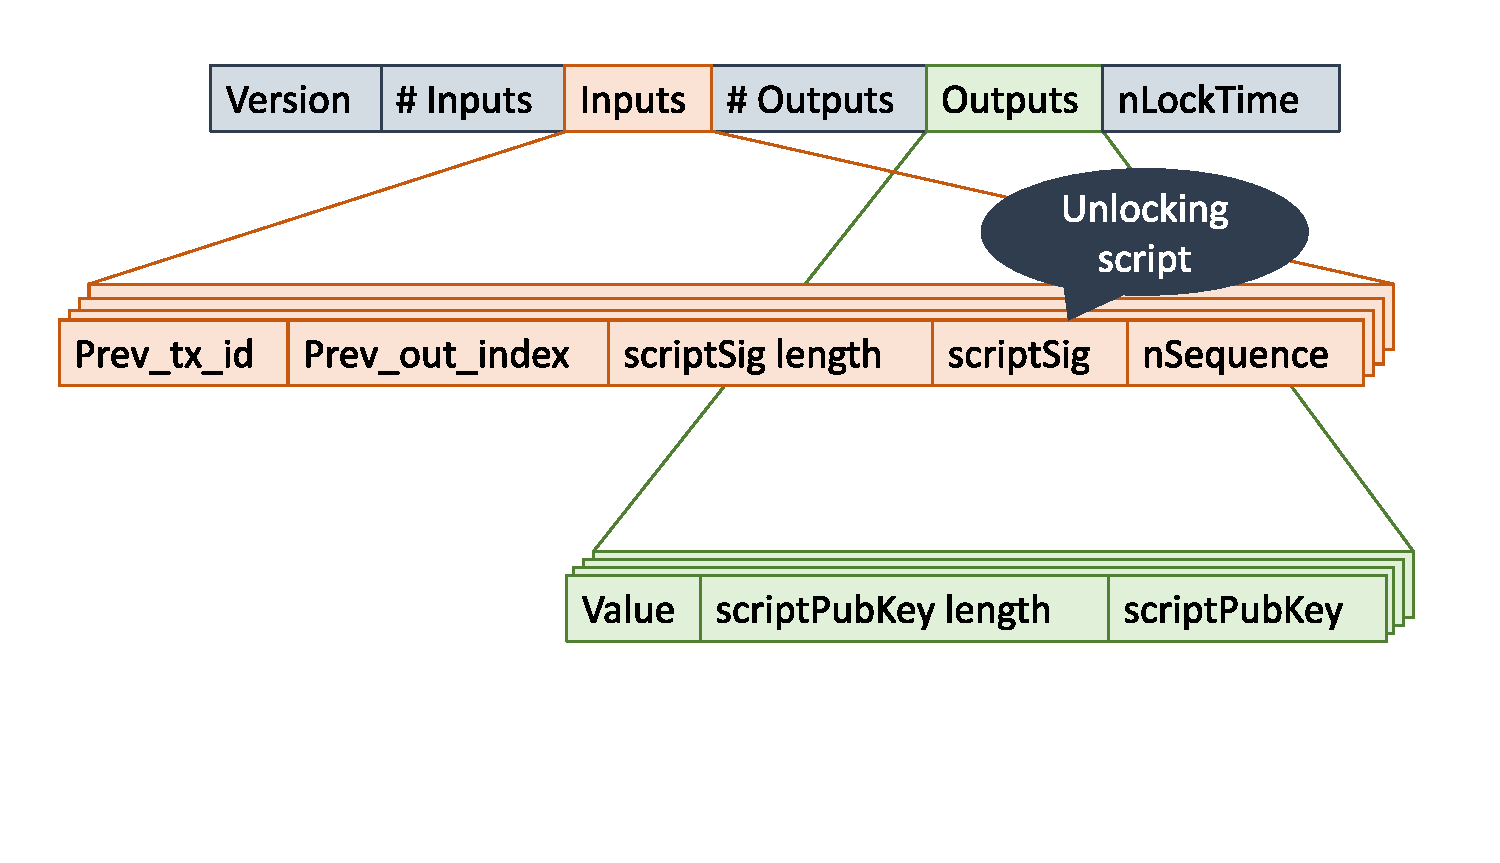
\includegraphics[width=\unitlength,page=1]{Figures/L2_transaction_struct.pdf}}%
  \end{picture}%
\endgroup%
    
\end{minipage}
TODO unlock/locking script\newline
\textbf{Common Bitcoin scripts}\newline
\begin{minipage}{0.5\linewidth}
    \centering      
    \def\svgwidth{\columnwidth}
    %% Creator: Inkscape inkscape 0.92.4, www.inkscape.org
%% PDF/EPS/PS + LaTeX output extension by Johan Engelen, 2010
%% Accompanies image file 'L2_bitcoin_scripts.pdf' (pdf, eps, ps)
%%
%% To include the image in your LaTeX document, write
%%   \input{<filename>.pdf_tex}
%%  instead of
%%   \includegraphics{<filename>.pdf}
%% To scale the image, write
%%   \def\svgwidth{<desired width>}
%%   \input{<filename>.pdf_tex}
%%  instead of
%%   \includegraphics[width=<desired width>]{<filename>.pdf}
%%
%% Images with a different path to the parent latex file can
%% be accessed with the `import' package (which may need to be
%% installed) using
%%   \usepackage{import}
%% in the preamble, and then including the image with
%%   \import{<path to file>}{<filename>.pdf_tex}
%% Alternatively, one can specify
%%   \graphicspath{{<path to file>/}}
%% 
%% For more information, please see info/svg-inkscape on CTAN:
%%   http://tug.ctan.org/tex-archive/info/svg-inkscape
%%
\begingroup%
  \makeatletter%
  \providecommand\color[2][]{%
    \errmessage{(Inkscape) Color is used for the text in Inkscape, but the package 'color.sty' is not loaded}%
    \renewcommand\color[2][]{}%
  }%
  \providecommand\transparent[1]{%
    \errmessage{(Inkscape) Transparency is used (non-zero) for the text in Inkscape, but the package 'transparent.sty' is not loaded}%
    \renewcommand\transparent[1]{}%
  }%
  \providecommand\rotatebox[2]{#2}%
  \newcommand*\fsize{\dimexpr\f@size pt\relax}%
  \newcommand*\lineheight[1]{\fontsize{\fsize}{#1\fsize}\selectfont}%
  \ifx\svgwidth\undefined%
    \setlength{\unitlength}{568.92860232bp}%
    \ifx\svgscale\undefined%
      \relax%
    \else%
      \setlength{\unitlength}{\unitlength * \real{\svgscale}}%
    \fi%
  \else%
    \setlength{\unitlength}{\svgwidth}%
  \fi%
  \global\let\svgwidth\undefined%
  \global\let\svgscale\undefined%
  \makeatother%
  \begin{picture}(1,0.5386064)%
    \lineheight{1}%
    \setlength\tabcolsep{0pt}%
    \put(0,0){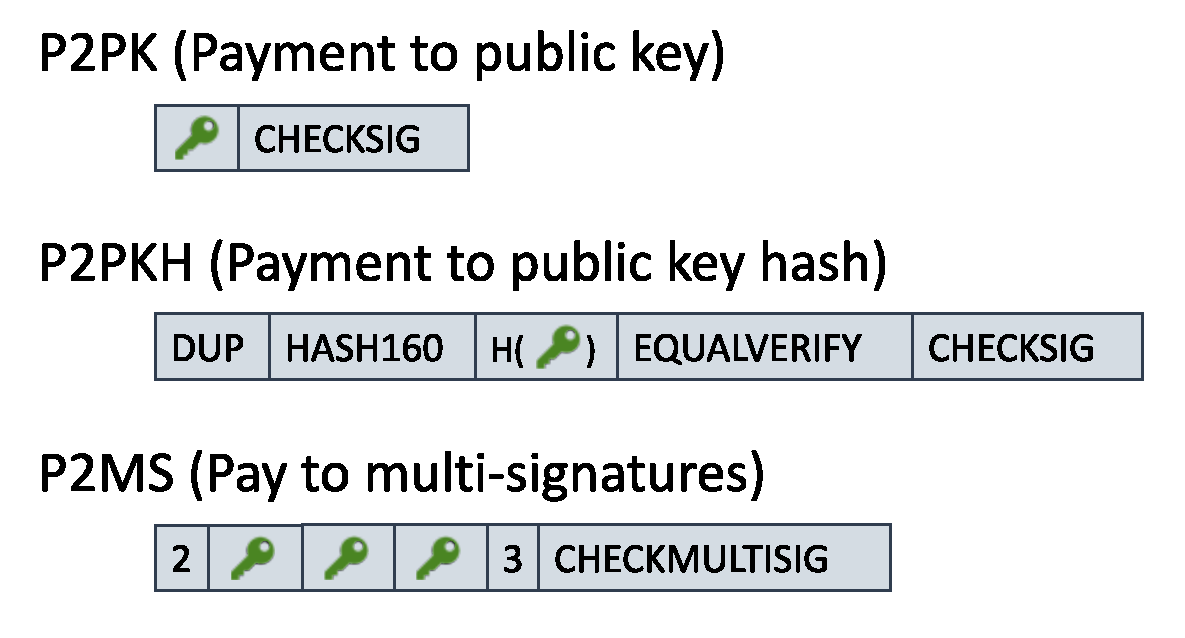
\includegraphics[width=\unitlength,page=1]{Figures/L2_bitcoin_scripts.pdf}}%
  \end{picture}%
\endgroup%
    
\end{minipage}
\paragraph{Bitcoin script Miscellaneous}
\begin{itemize}
    \item BitML: Language for Bitcoin smart contracts
    \item Oracles
    \item Escrow and arbitration
    \item Fair multi-party lotteries
    \item Gambling games (Poker)
    \item Crowdfunding
\end{itemize}{}
\paragraph{Bitcoin scripts Restrictions}
\begin{itemize}
    \item No loops
    \item No signature verification on arbitrary messages
    \item No multiplication and shifting
    \item No arithmetic on long numbers
    \item No concatenation on bitstrings
\end{itemize}

\section{Ethereum and smart contracts}
\subsection{Smart Contracts and Ethereum}

\paragraph{Smart contract:}
\begin{itemize}
    \item computerized transaction protocol, that executes the terms of a contract.
    \item Minimizes the need for trusted intermediaries.
\end{itemize}{}

\paragraph{Ethereum:}
\begin{itemize}
    \item A decentralized platform designed to run smart contracts.
    \item Eth smart contracts are Turing-complete.
    \item Transactions change the state of one or more contracts.
    \item Latest block stores the latest local state of all smart contracts.
    \item Difference to Bitcoin:
    \begin{itemize}
        \item In Eth we own private keys to an account, not to a set of unspent transactions.
        \item In this account the balance is updated, we don't simply store unspent transactions.
        \item Account contains executable code.
    \end{itemize}{}
\end{itemize}{}

\paragraph{Ethereum accounts:}
\begin{itemize}
    \item \textbf{User accounts:} Owned by some person
    \begin{itemize}
        \item Can send transactions to transfer ether or trigger contract code.
        \item Contains Address and Ether balance.
    \end{itemize}
    \item \textbf{Contract accounts: } Owned by contract (autonomous).
    \begin{itemize}
        \item Code execution triggered by transactions that call functions.
        \item Contains Address, Ether balance, Associated contract code and persistent storage (state)
    \end{itemize}{}
\end{itemize}{}

\paragraph{Writing smart contracts:} Multiple high-level languages (Solidity, Vyper) and single low-level language (EVM bytecode). 

\begin{minipage}{0.75\linewidth}
    \centering      
    \def\svgwidth{\linewidth}
    %% Creator: Inkscape inkscape 0.92.4, www.inkscape.org
%% PDF/EPS/PS + LaTeX output extension by Johan Engelen, 2010
%% Accompanies image file 'L3_transactions.pdf' (pdf, eps, ps)
%%
%% To include the image in your LaTeX document, write
%%   \input{<filename>.pdf_tex}
%%  instead of
%%   \includegraphics{<filename>.pdf}
%% To scale the image, write
%%   \def\svgwidth{<desired width>}
%%   \input{<filename>.pdf_tex}
%%  instead of
%%   \includegraphics[width=<desired width>]{<filename>.pdf}
%%
%% Images with a different path to the parent latex file can
%% be accessed with the `import' package (which may need to be
%% installed) using
%%   \usepackage{import}
%% in the preamble, and then including the image with
%%   \import{<path to file>}{<filename>.pdf_tex}
%% Alternatively, one can specify
%%   \graphicspath{{<path to file>/}}
%% 
%% For more information, please see info/svg-inkscape on CTAN:
%%   http://tug.ctan.org/tex-archive/info/svg-inkscape
%%
\begingroup%
  \makeatletter%
  \providecommand\color[2][]{%
    \errmessage{(Inkscape) Color is used for the text in Inkscape, but the package 'color.sty' is not loaded}%
    \renewcommand\color[2][]{}%
  }%
  \providecommand\transparent[1]{%
    \errmessage{(Inkscape) Transparency is used (non-zero) for the text in Inkscape, but the package 'transparent.sty' is not loaded}%
    \renewcommand\transparent[1]{}%
  }%
  \providecommand\rotatebox[2]{#2}%
  \newcommand*\fsize{\dimexpr\f@size pt\relax}%
  \newcommand*\lineheight[1]{\fontsize{\fsize}{#1\fsize}\selectfont}%
  \ifx\svgwidth\undefined%
    \setlength{\unitlength}{720bp}%
    \ifx\svgscale\undefined%
      \relax%
    \else%
      \setlength{\unitlength}{\unitlength * \real{\svgscale}}%
    \fi%
  \else%
    \setlength{\unitlength}{\svgwidth}%
  \fi%
  \global\let\svgwidth\undefined%
  \global\let\svgscale\undefined%
  \makeatother%
  \begin{picture}(1,0.75)%
    \lineheight{1}%
    \setlength\tabcolsep{0pt}%
    \put(0,0){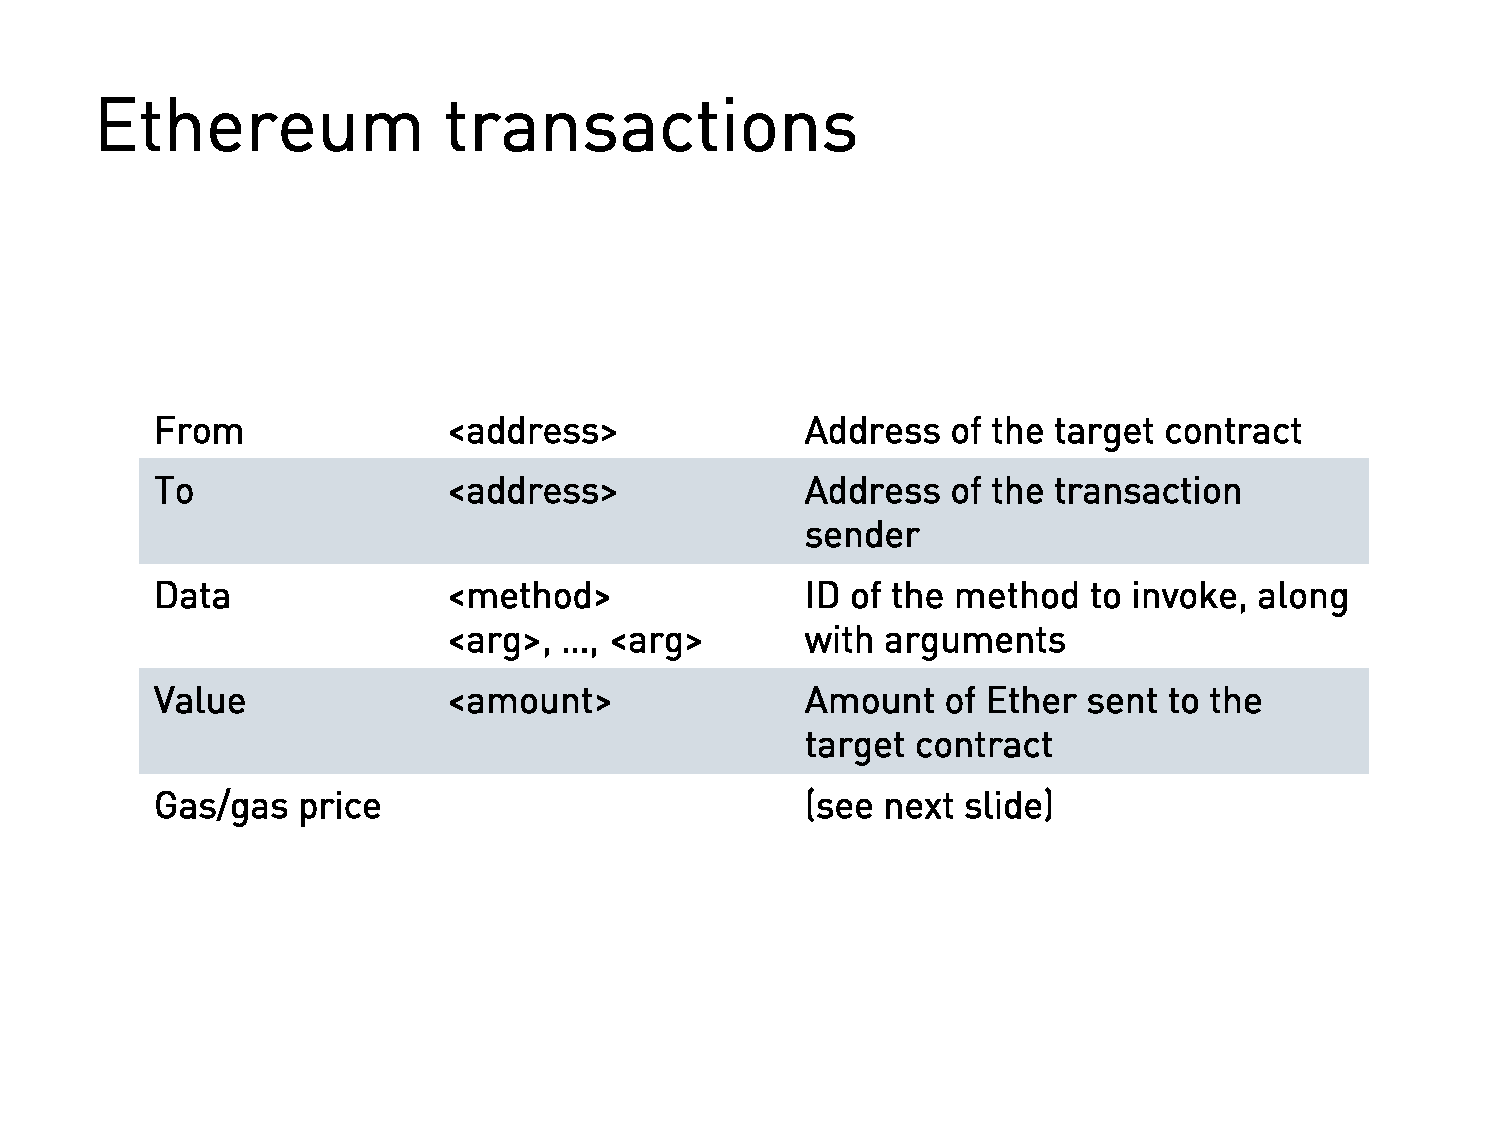
\includegraphics[width=\unitlength,page=1]{Figures/L3_transactions.pdf}}%
  \end{picture}%
\endgroup%



    
\end{minipage}

\paragraph{Gas: } How to prevent infinite loops in contract?
\begin{itemize}
    \item A transaction requires gas to fuel contract execution.
    \item Each EVM opcode has its amount of gas, it needs in order to be executed.
    \item Every transaction specifies a maximum amount of gas the sender is willing to spend.
    \item If the contract successfully executes, the unspent gas money is refunded to the sender.
    \item If execution runs out of gas, the execution is reverted, but gas money is not refunded.
    \item[\color{red}{$\xrightarrow{}$}] \textcolor{red}{Exploit:} The attacker can craft a transaction that triggers an out-of-gas exception at an arbitrary point in the execution. May create undesirable behaviors if not entire transaction is reverted.
\end{itemize}{}

\paragraph{Ether transfers:}
\begin{itemize}
    \item An ether transfer to a contract implicitly calls the receiver contract (called contract takes control over the execution).
    \item[\color{red}{$\xrightarrow{}$}] \textcolor{red}{Exploit:} Thus an attacker may own the external contract and execute arbitrary code. In particular, he can call back the contract before returning control to the caller.
    \item Any user can call arbitrary functions in contracts unless they have a \texttt{require(statement)} clause. This reverts the transaction if the statement is false
\end{itemize}{}

\begin{minipage}{0.75\linewidth}
    \centering      
    \def\svgwidth{\linewidth}
    %% Creator: Inkscape inkscape 0.92.4, www.inkscape.org
%% PDF/EPS/PS + LaTeX output extension by Johan Engelen, 2010
%% Accompanies image file 'ether_transfer_types.pdf' (pdf, eps, ps)
%%
%% To include the image in your LaTeX document, write
%%   \input{<filename>.pdf_tex}
%%  instead of
%%   \includegraphics{<filename>.pdf}
%% To scale the image, write
%%   \def\svgwidth{<desired width>}
%%   \input{<filename>.pdf_tex}
%%  instead of
%%   \includegraphics[width=<desired width>]{<filename>.pdf}
%%
%% Images with a different path to the parent latex file can
%% be accessed with the `import' package (which may need to be
%% installed) using
%%   \usepackage{import}
%% in the preamble, and then including the image with
%%   \import{<path to file>}{<filename>.pdf_tex}
%% Alternatively, one can specify
%%   \graphicspath{{<path to file>/}}
%% 
%% For more information, please see info/svg-inkscape on CTAN:
%%   http://tug.ctan.org/tex-archive/info/svg-inkscape
%%
\begingroup%
  \makeatletter%
  \providecommand\color[2][]{%
    \errmessage{(Inkscape) Color is used for the text in Inkscape, but the package 'color.sty' is not loaded}%
    \renewcommand\color[2][]{}%
  }%
  \providecommand\transparent[1]{%
    \errmessage{(Inkscape) Transparency is used (non-zero) for the text in Inkscape, but the package 'transparent.sty' is not loaded}%
    \renewcommand\transparent[1]{}%
  }%
  \providecommand\rotatebox[2]{#2}%
  \newcommand*\fsize{\dimexpr\f@size pt\relax}%
  \newcommand*\lineheight[1]{\fontsize{\fsize}{#1\fsize}\selectfont}%
  \ifx\svgwidth\undefined%
    \setlength{\unitlength}{730.7812546bp}%
    \ifx\svgscale\undefined%
      \relax%
    \else%
      \setlength{\unitlength}{\unitlength * \real{\svgscale}}%
    \fi%
  \else%
    \setlength{\unitlength}{\svgwidth}%
  \fi%
  \global\let\svgwidth\undefined%
  \global\let\svgscale\undefined%
  \makeatother%
  \begin{picture}(1,0.73893521)%
    \lineheight{1}%
    \setlength\tabcolsep{0pt}%
    \put(0,0){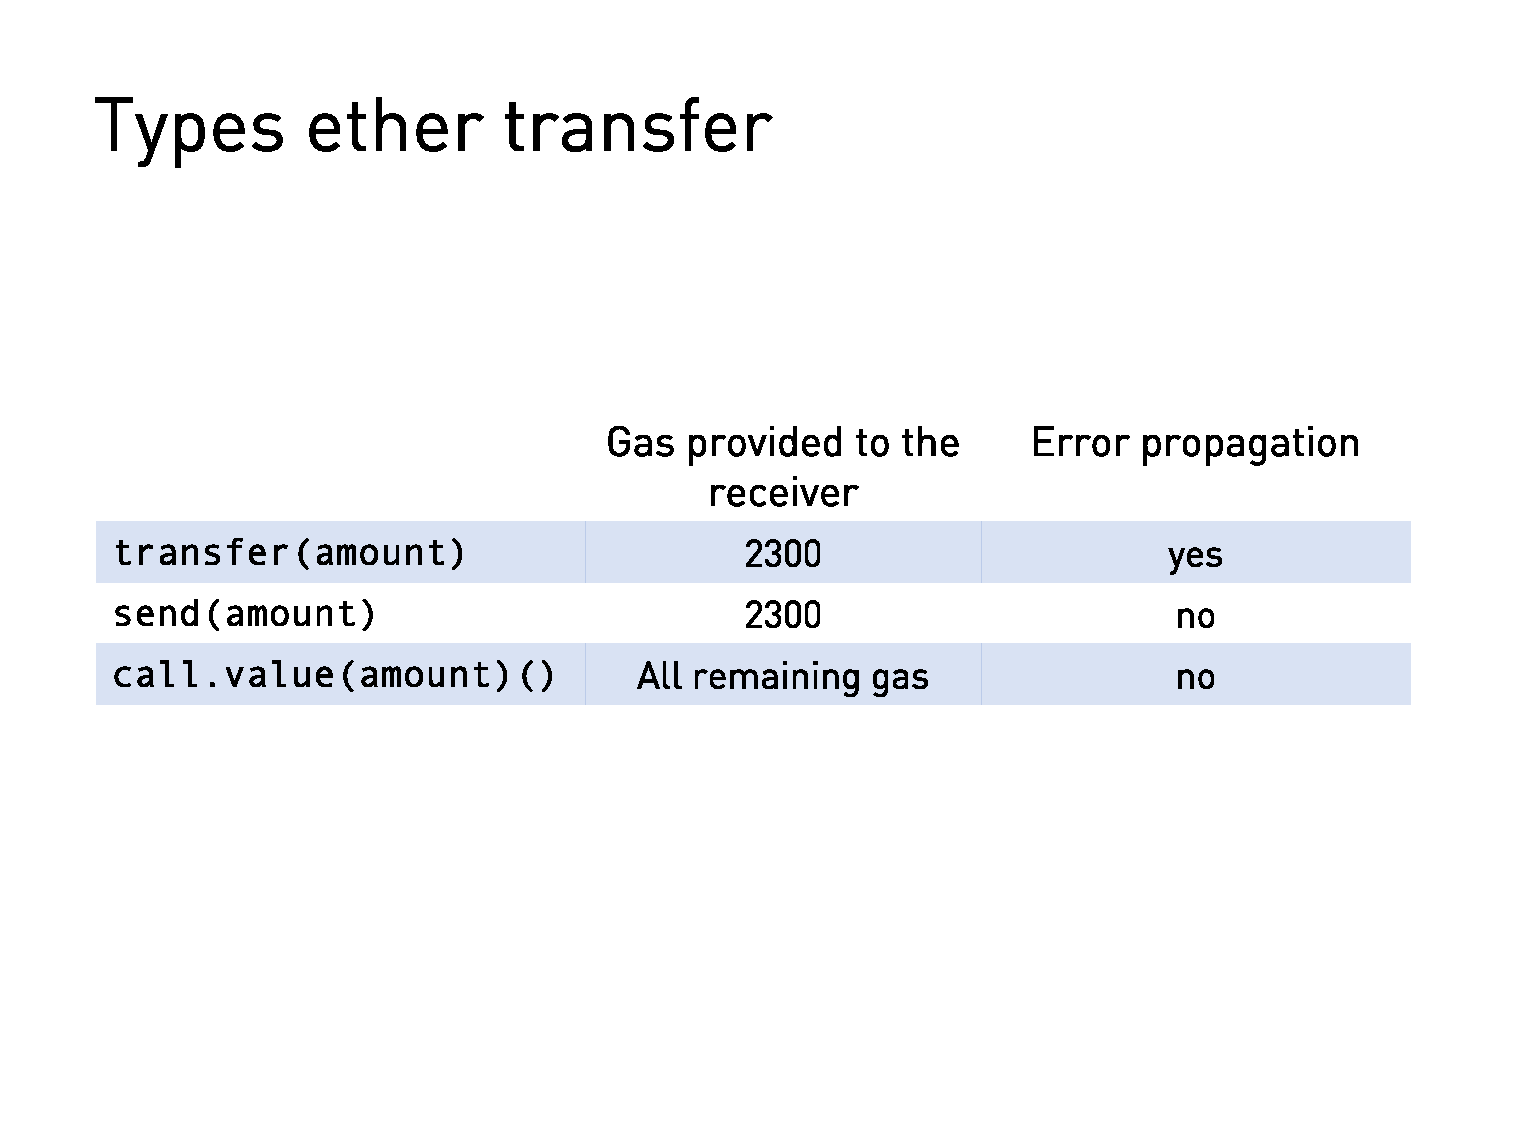
\includegraphics[width=\unitlength,page=1]{Figures/L3_ether_transfer_types.pdf}}%
  \end{picture}%
\endgroup%
    
\end{minipage}

\paragraph{Storage model} In the following variableID and mappingsId are just numbers that identify the variable (e.g. 0 for variable0, 1 for variable1, ..). 
\begin{itemize}
    \item \textbf{Variables:} value stored at \textcolor{blue}{offset} = $variableID$
    \item \textbf{Mappings:} mapping[key] stored at \textcolor{blue}{offset} = $SHA3(mappingID||key)$ 
    \item \textbf{Arrays:} array[10] stored at \textcolor{blue}{offset} = $SHA3(arrayID) + 10$
\end{itemize}{}

\subsection{Vulnerabilities of Smart Contracts}

\begin{enumerate}
    \item \textbf{The DAO bug:} Call \texttt{withdraw()} twice, first normally, then again before balance is set to zero.
    \item \textbf{BatchOverflow Exploit: }
\end{enumerate}{}

\begin{minipage}{0.45\linewidth}
    \centering      
    \def\svgwidth{\linewidth}
    %% Creator: Inkscape inkscape 0.92.4, www.inkscape.org
%% PDF/EPS/PS + LaTeX output extension by Johan Engelen, 2010
%% Accompanies image file 'L3_dao_bug.pdf' (pdf, eps, ps)
%%
%% To include the image in your LaTeX document, write
%%   \input{<filename>.pdf_tex}
%%  instead of
%%   \includegraphics{<filename>.pdf}
%% To scale the image, write
%%   \def\svgwidth{<desired width>}
%%   \input{<filename>.pdf_tex}
%%  instead of
%%   \includegraphics[width=<desired width>]{<filename>.pdf}
%%
%% Images with a different path to the parent latex file can
%% be accessed with the `import' package (which may need to be
%% installed) using
%%   \usepackage{import}
%% in the preamble, and then including the image with
%%   \import{<path to file>}{<filename>.pdf_tex}
%% Alternatively, one can specify
%%   \graphicspath{{<path to file>/}}
%% 
%% For more information, please see info/svg-inkscape on CTAN:
%%   http://tug.ctan.org/tex-archive/info/svg-inkscape
%%
\begingroup%
  \makeatletter%
  \providecommand\color[2][]{%
    \errmessage{(Inkscape) Color is used for the text in Inkscape, but the package 'color.sty' is not loaded}%
    \renewcommand\color[2][]{}%
  }%
  \providecommand\transparent[1]{%
    \errmessage{(Inkscape) Transparency is used (non-zero) for the text in Inkscape, but the package 'transparent.sty' is not loaded}%
    \renewcommand\transparent[1]{}%
  }%
  \providecommand\rotatebox[2]{#2}%
  \newcommand*\fsize{\dimexpr\f@size pt\relax}%
  \newcommand*\lineheight[1]{\fontsize{\fsize}{#1\fsize}\selectfont}%
  \ifx\svgwidth\undefined%
    \setlength{\unitlength}{720.00000454bp}%
    \ifx\svgscale\undefined%
      \relax%
    \else%
      \setlength{\unitlength}{\unitlength * \real{\svgscale}}%
    \fi%
  \else%
    \setlength{\unitlength}{\svgwidth}%
  \fi%
  \global\let\svgwidth\undefined%
  \global\let\svgscale\undefined%
  \makeatother%
  \begin{picture}(1,0.75)%
    \lineheight{1}%
    \setlength\tabcolsep{0pt}%
    \put(0,0){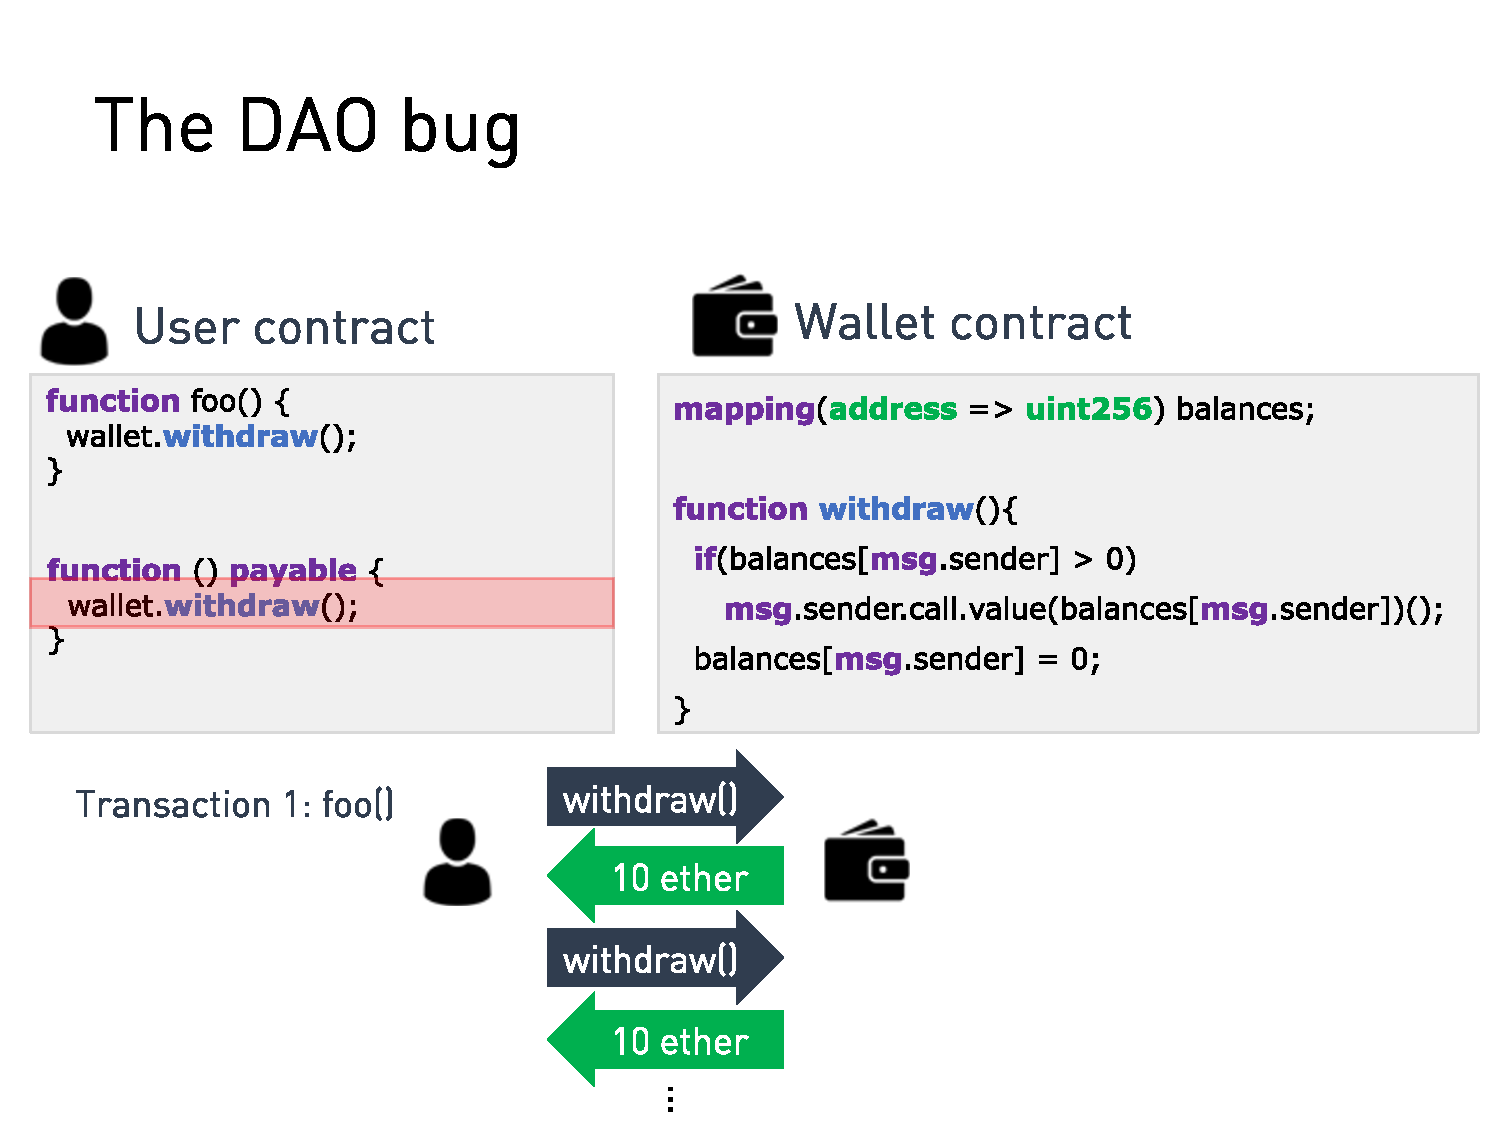
\includegraphics[width=\unitlength,page=1]{Figures/L3_dao_bug.pdf}}%
  \end{picture}%
\endgroup%
    
\end{minipage}
\begin{minipage}{0.45\linewidth}
    \centering      
    \def\svgwidth{\linewidth}
    %% Creator: Inkscape inkscape 0.92.4, www.inkscape.org
%% PDF/EPS/PS + LaTeX output extension by Johan Engelen, 2010
%% Accompanies image file 'L3_overflow_exploit.pdf' (pdf, eps, ps)
%%
%% To include the image in your LaTeX document, write
%%   \input{<filename>.pdf_tex}
%%  instead of
%%   \includegraphics{<filename>.pdf}
%% To scale the image, write
%%   \def\svgwidth{<desired width>}
%%   \input{<filename>.pdf_tex}
%%  instead of
%%   \includegraphics[width=<desired width>]{<filename>.pdf}
%%
%% Images with a different path to the parent latex file can
%% be accessed with the `import' package (which may need to be
%% installed) using
%%   \usepackage{import}
%% in the preamble, and then including the image with
%%   \import{<path to file>}{<filename>.pdf_tex}
%% Alternatively, one can specify
%%   \graphicspath{{<path to file>/}}
%% 
%% For more information, please see info/svg-inkscape on CTAN:
%%   http://tug.ctan.org/tex-archive/info/svg-inkscape
%%
\begingroup%
  \makeatletter%
  \providecommand\color[2][]{%
    \errmessage{(Inkscape) Color is used for the text in Inkscape, but the package 'color.sty' is not loaded}%
    \renewcommand\color[2][]{}%
  }%
  \providecommand\transparent[1]{%
    \errmessage{(Inkscape) Transparency is used (non-zero) for the text in Inkscape, but the package 'transparent.sty' is not loaded}%
    \renewcommand\transparent[1]{}%
  }%
  \providecommand\rotatebox[2]{#2}%
  \newcommand*\fsize{\dimexpr\f@size pt\relax}%
  \newcommand*\lineheight[1]{\fontsize{\fsize}{#1\fsize}\selectfont}%
  \ifx\svgwidth\undefined%
    \setlength{\unitlength}{720.00000454bp}%
    \ifx\svgscale\undefined%
      \relax%
    \else%
      \setlength{\unitlength}{\unitlength * \real{\svgscale}}%
    \fi%
  \else%
    \setlength{\unitlength}{\svgwidth}%
  \fi%
  \global\let\svgwidth\undefined%
  \global\let\svgscale\undefined%
  \makeatother%
  \begin{picture}(1,0.75)%
    \lineheight{1}%
    \setlength\tabcolsep{0pt}%
    \put(0,0){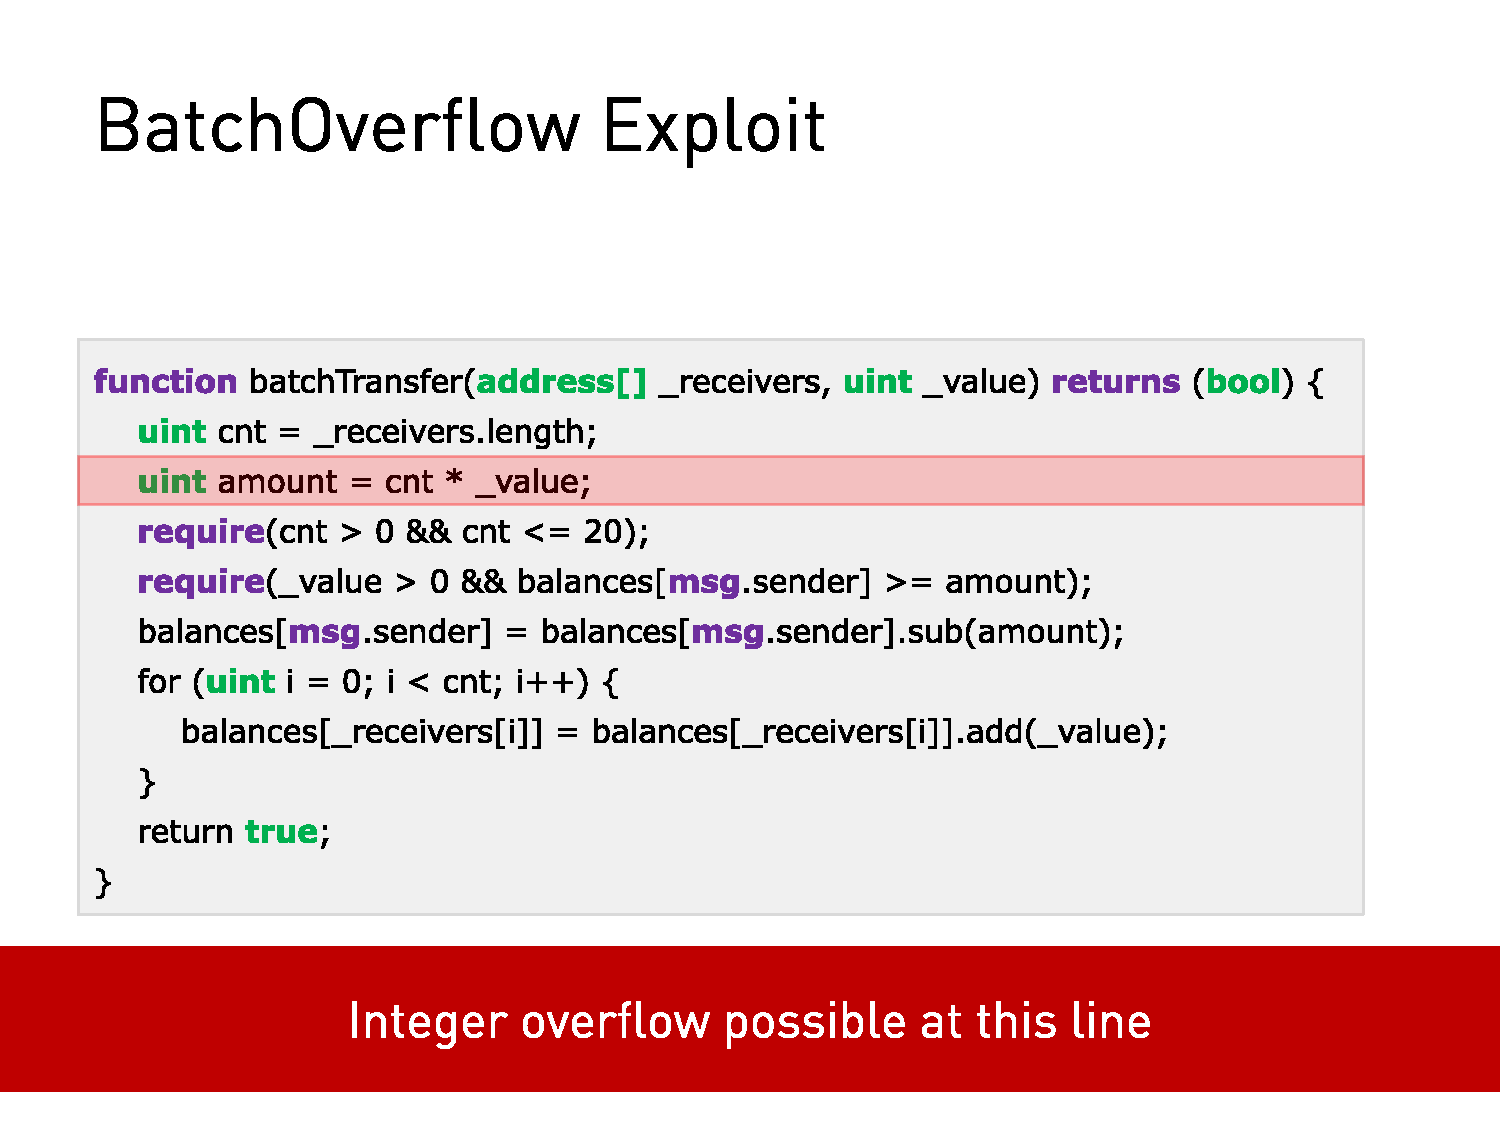
\includegraphics[width=\unitlength,page=1]{Figures/L3_overflow_exploit.pdf}}%
  \end{picture}%
\endgroup%
    
\end{minipage}

\subsection{Semantics and Security Properties}
\begin{itemize}
    \item \textbf{Ethereum virtual machine (EVM) state:} \textcolor{blue}{$\sigma = (S,M,Q,B)$}
    \begin{itemize}
        \item \textcolor{orange}{Storage [S]:} Persistent, inital storage is defined by the constructor.
        \item \textcolor{orange}{Memory [M]:} Not-persistent, re-initialized before  executing a transaction.
        \item \textcolor{orange}{Stack [Q]:} Each element is 256 bits.
        \item \textcolor{orange}{Block information [B]:} Number, timestamp, etc. Fixed for a given transaction.
    \end{itemize}{}
    \item \textbf{Transaction: } \textcolor{blue}{$T = (\texttt{caller}, \texttt{func}, \texttt{args})$}
    \item \textbf{Correctness of smart contracts:} \textcolor{blue}{$\texttt{SmartContract} \implies \texttt{Func/Sec
    Properties}$} 
    \begin{itemize}
        \item Check formal properties for all states.
    \end{itemize}{}
\end{itemize}{}
\section{Fuzzing}
\subsection{Fuzzer Basics}
\paragraph{Fuzzer pipeline:\newline}
\begin{minipage}{0.75\linewidth}
    \centering      
    \def\svgwidth{\linewidth}
    %% Creator: Inkscape inkscape 0.92.4, www.inkscape.org
%% PDF/EPS/PS + LaTeX output extension by Johan Engelen, 2010
%% Accompanies image file 'L4_fuzzer_pipeline.pdf' (pdf, eps, ps)
%%
%% To include the image in your LaTeX document, write
%%   \input{<filename>.pdf_tex}
%%  instead of
%%   \includegraphics{<filename>.pdf}
%% To scale the image, write
%%   \def\svgwidth{<desired width>}
%%   \input{<filename>.pdf_tex}
%%  instead of
%%   \includegraphics[width=<desired width>]{<filename>.pdf}
%%
%% Images with a different path to the parent latex file can
%% be accessed with the `import' package (which may need to be
%% installed) using
%%   \usepackage{import}
%% in the preamble, and then including the image with
%%   \import{<path to file>}{<filename>.pdf_tex}
%% Alternatively, one can specify
%%   \graphicspath{{<path to file>/}}
%% 
%% For more information, please see info/svg-inkscape on CTAN:
%%   http://tug.ctan.org/tex-archive/info/svg-inkscape
%%
\begingroup%
  \makeatletter%
  \providecommand\color[2][]{%
    \errmessage{(Inkscape) Color is used for the text in Inkscape, but the package 'color.sty' is not loaded}%
    \renewcommand\color[2][]{}%
  }%
  \providecommand\transparent[1]{%
    \errmessage{(Inkscape) Transparency is used (non-zero) for the text in Inkscape, but the package 'transparent.sty' is not loaded}%
    \renewcommand\transparent[1]{}%
  }%
  \providecommand\rotatebox[2]{#2}%
  \newcommand*\fsize{\dimexpr\f@size pt\relax}%
  \newcommand*\lineheight[1]{\fontsize{\fsize}{#1\fsize}\selectfont}%
  \ifx\svgwidth\undefined%
    \setlength{\unitlength}{720bp}%
    \ifx\svgscale\undefined%
      \relax%
    \else%
      \setlength{\unitlength}{\unitlength * \real{\svgscale}}%
    \fi%
  \else%
    \setlength{\unitlength}{\svgwidth}%
  \fi%
  \global\let\svgwidth\undefined%
  \global\let\svgscale\undefined%
  \makeatother%
  \begin{picture}(1,0.75)%
    \lineheight{1}%
    \setlength\tabcolsep{0pt}%
    \put(0,0){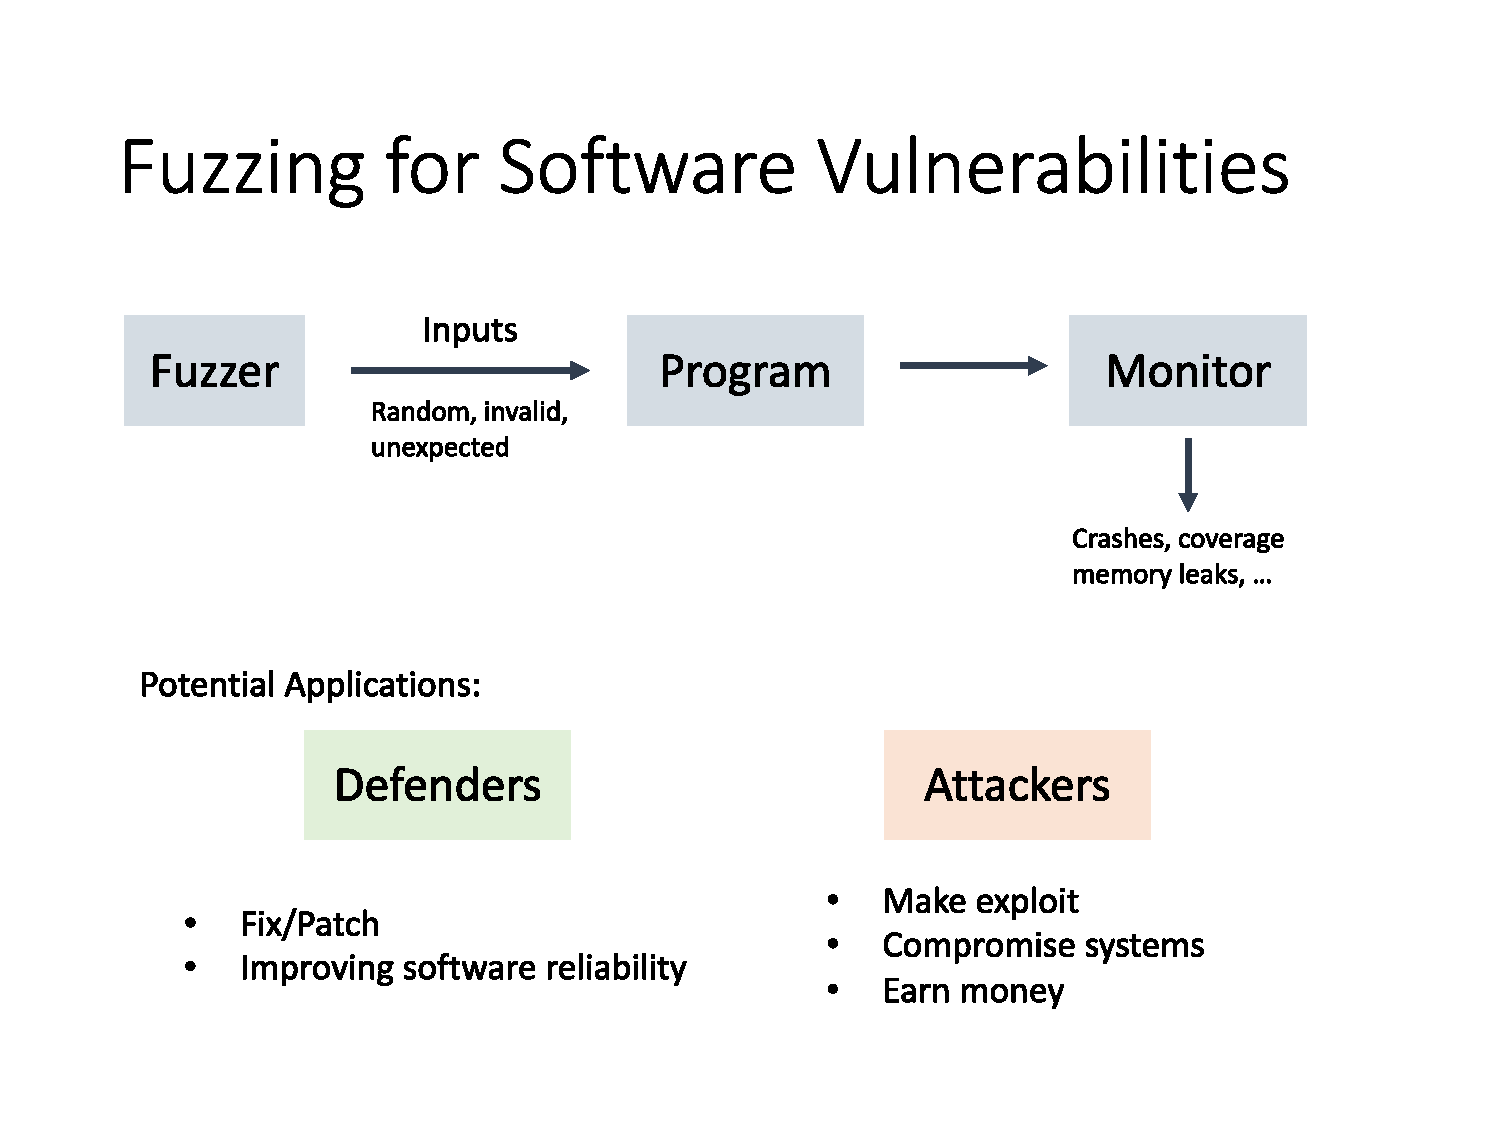
\includegraphics[width=\unitlength,page=1]{Figures/L4_fuzzer_pipeline.pdf}}%
  \end{picture}%
\endgroup%
    
\end{minipage}

\begin{multicols}{2}
 \textbf{Functional Testing}  \\ \rule{\linewidth}{0.4pt} \\ Run programs on \textcolor{green}{well-structured} and \textcolor{green}{normal} inputs (e.g., unit tests) \\ \\ Prevent \textcolor{green}{normal users} from encountering functionality errors  (e.g., assertion failures) 
 \columnbreak 
 \\ \textbf{Fuzzing}  \\ \rule{\linewidth}{0.4pt}  \\ Test programs on \textcolor{red}{abnormal} inputs (e.g., randomly generated \\ \\ Prevent \textcolor{red}{attackers} from making exploits (e.g., memory leaks)
 
\end{multicols}


\paragraph{Fuzzer Categories:}
\begin{description}
    \item \textbf{\textcolor{blue}{Black-Box}} \textbf{No information} about the program or inputs \textcolor{green}{Easy-to-use and fast}, but \textcolor{red}{only explore shallow states}
    \item \textbf{\textcolor{blue}{Grammar-based}} Generate inputs specified a \textbf{grammar}. \textcolor{green}{Can reach deeper states}, but \textcolor{red}{assume a grammar}
    \item \textbf{\textcolor{blue}{White-box}} Use \textbf{heavy-weight program analysis} to generate inputs. \textcolor{green}{Can reach deeper states}, but \textcolor{red}{computationally expensive}
    \item \textbf{\textcolor{blue}{Grey-box}} Use \textbf{light-weight} instrumentation for getting input coverage. \textcolor{green}{Can reach deeper states }, but \textcolor{red}{need careful tuning}
\end{description}{}
\paragraph{Fuzzing Inputs:}
\begin{itemize}
    \item \textbf{\textcolor{blue}{Mutation}} Mutate from "good" seed inputs
        \begin{itemize}
            \item[\color{green}+] Easy to setup
            \item[\color{green}+] No input format specification required
            \item[\color{red}--] Seed inputs required
            \item[\color{red}--] May fail for complex functions (e.g., checksum)
        \end{itemize}
    \item \textbf{\textcolor{blue}{Generation}} Generate inputs from scratch, usually by a grammar
    \begin{itemize} 
        \item[\color{green}+] No need for seed inputs
        \item[\color{red}--] Labor expensive to write generators 
        \item[\color{red}--] Input formed specification required
    \end{itemize}
\end{itemize}
\paragraph{American Fuzzy Loop \textbf{AFL}:}
\begin{itemize}
    \item AFL is a mutational, grey-box fuzzer, with (compile-time or binary-level) instrumentation for branch coverage
    \item Starts a queue from a set of seed inputs
    \item Generates new test cases by mutation from the queue:
    \begin{itemize}
        \item bit or byte flips
        \item addition or subtraction of small integers to bytes
        \item test cases splicing
    \end{itemize}
    \item Add new test case to the queue if new branches are triggered.
\end{itemize}

TODO ILF and Compiler fuzzing examples
\subsection{Symbolic Execution}
\begin{itemize}
\item We associate each variables with a \textcolor{green}{symbolic value} instead of a concrete value.
\item We then run the program with the symbolic values, and obtain a \textcolor{green}{constraint formula}
\item At any program point, we can invoke a constraint (SMT) solver to find \textcolor{green}{satisfying assignments} to the formula, which can be used to indicate \textcolor{green}{concrete inputs} reaching the program point.
\end{itemize}{}

\paragraph{Tracking:}
Symbolic Execution tracks the following two formulas:
\begin{itemize}
    \item \textcolor{green}{symbolic store}: Tracks possible values of variables
    \item \textcolor{green}{path constraint}: Tracks history of all branches taken so far
\end{itemize}{}
\textcolor{green}{Symbolic state} is then defined as the \textcolor{green}{conjunction} of these two formulas
\paragraph{Example:\newline}

\noindent\begin{minipage}{0.5\linewidth}
    \centering      
    \def\svgwidth{\linewidth}
    %% Creator: Inkscape inkscape 0.92.4, www.inkscape.org
%% PDF/EPS/PS + LaTeX output extension by Johan Engelen, 2010
%% Accompanies image file 'L4_symbolic_execution_example_1.pdf' (pdf, eps, ps)
%%
%% To include the image in your LaTeX document, write
%%   \input{<filename>.pdf_tex}
%%  instead of
%%   \includegraphics{<filename>.pdf}
%% To scale the image, write
%%   \def\svgwidth{<desired width>}
%%   \input{<filename>.pdf_tex}
%%  instead of
%%   \includegraphics[width=<desired width>]{<filename>.pdf}
%%
%% Images with a different path to the parent latex file can
%% be accessed with the `import' package (which may need to be
%% installed) using
%%   \usepackage{import}
%% in the preamble, and then including the image with
%%   \import{<path to file>}{<filename>.pdf_tex}
%% Alternatively, one can specify
%%   \graphicspath{{<path to file>/}}
%% 
%% For more information, please see info/svg-inkscape on CTAN:
%%   http://tug.ctan.org/tex-archive/info/svg-inkscape
%%
\begingroup%
  \makeatletter%
  \providecommand\color[2][]{%
    \errmessage{(Inkscape) Color is used for the text in Inkscape, but the package 'color.sty' is not loaded}%
    \renewcommand\color[2][]{}%
  }%
  \providecommand\transparent[1]{%
    \errmessage{(Inkscape) Transparency is used (non-zero) for the text in Inkscape, but the package 'transparent.sty' is not loaded}%
    \renewcommand\transparent[1]{}%
  }%
  \providecommand\rotatebox[2]{#2}%
  \newcommand*\fsize{\dimexpr\f@size pt\relax}%
  \newcommand*\lineheight[1]{\fontsize{\fsize}{#1\fsize}\selectfont}%
  \ifx\svgwidth\undefined%
    \setlength{\unitlength}{596.55861201bp}%
    \ifx\svgscale\undefined%
      \relax%
    \else%
      \setlength{\unitlength}{\unitlength * \real{\svgscale}}%
    \fi%
  \else%
    \setlength{\unitlength}{\svgwidth}%
  \fi%
  \global\let\svgwidth\undefined%
  \global\let\svgscale\undefined%
  \makeatother%
  \begin{picture}(1,0.61038899)%
    \lineheight{1}%
    \setlength\tabcolsep{0pt}%
    \put(0,0){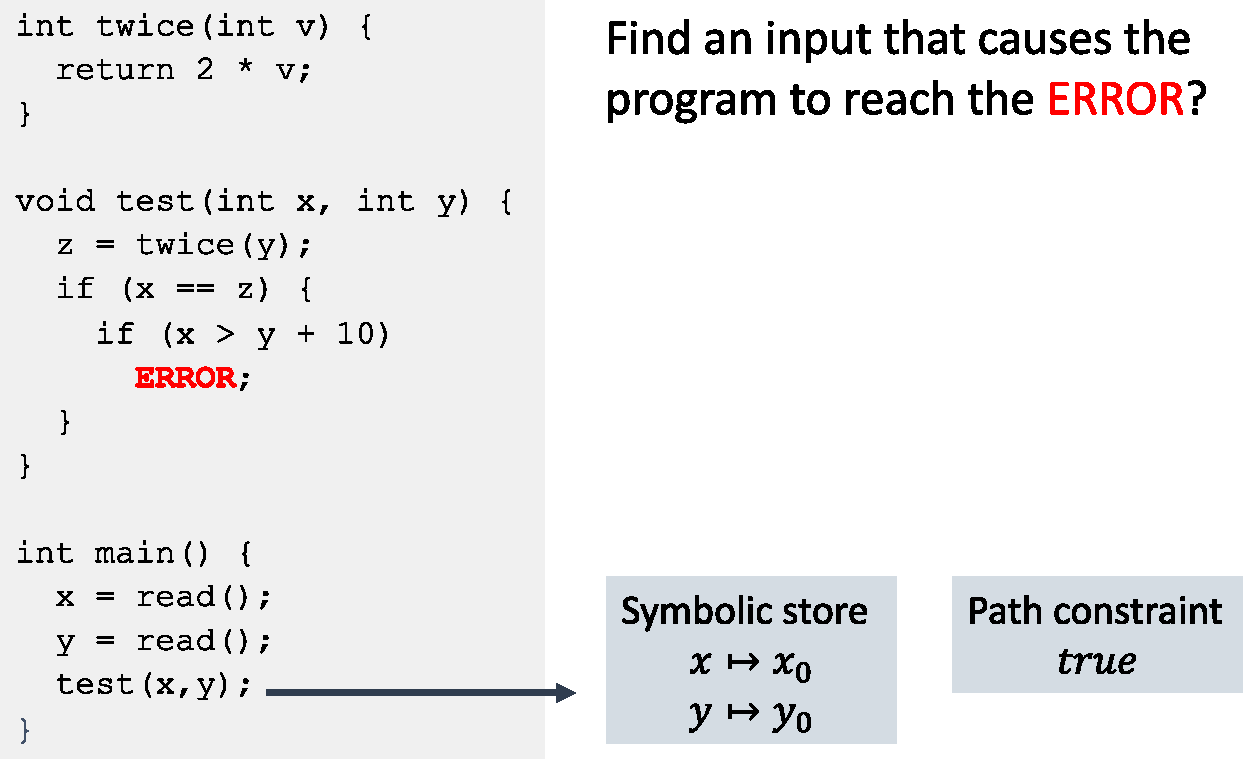
\includegraphics[width=\unitlength,page=1]{Figures/L4_symbolic_execution_example_1.pdf}}%
  \end{picture}%
\endgroup%
    
\end{minipage}
\begin{minipage}{0.5\linewidth}
    \centering      
    \def\svgwidth{\linewidth}
    %% Creator: Inkscape inkscape 0.92.4, www.inkscape.org
%% PDF/EPS/PS + LaTeX output extension by Johan Engelen, 2010
%% Accompanies image file 'L4_symbolic_execution_example_2.pdf' (pdf, eps, ps)
%%
%% To include the image in your LaTeX document, write
%%   \input{<filename>.pdf_tex}
%%  instead of
%%   \includegraphics{<filename>.pdf}
%% To scale the image, write
%%   \def\svgwidth{<desired width>}
%%   \input{<filename>.pdf_tex}
%%  instead of
%%   \includegraphics[width=<desired width>]{<filename>.pdf}
%%
%% Images with a different path to the parent latex file can
%% be accessed with the `import' package (which may need to be
%% installed) using
%%   \usepackage{import}
%% in the preamble, and then including the image with
%%   \import{<path to file>}{<filename>.pdf_tex}
%% Alternatively, one can specify
%%   \graphicspath{{<path to file>/}}
%% 
%% For more information, please see info/svg-inkscape on CTAN:
%%   http://tug.ctan.org/tex-archive/info/svg-inkscape
%%
\begingroup%
  \makeatletter%
  \providecommand\color[2][]{%
    \errmessage{(Inkscape) Color is used for the text in Inkscape, but the package 'color.sty' is not loaded}%
    \renewcommand\color[2][]{}%
  }%
  \providecommand\transparent[1]{%
    \errmessage{(Inkscape) Transparency is used (non-zero) for the text in Inkscape, but the package 'transparent.sty' is not loaded}%
    \renewcommand\transparent[1]{}%
  }%
  \providecommand\rotatebox[2]{#2}%
  \newcommand*\fsize{\dimexpr\f@size pt\relax}%
  \newcommand*\lineheight[1]{\fontsize{\fsize}{#1\fsize}\selectfont}%
  \ifx\svgwidth\undefined%
    \setlength{\unitlength}{610.37889375bp}%
    \ifx\svgscale\undefined%
      \relax%
    \else%
      \setlength{\unitlength}{\unitlength * \real{\svgscale}}%
    \fi%
  \else%
    \setlength{\unitlength}{\svgwidth}%
  \fi%
  \global\let\svgwidth\undefined%
  \global\let\svgscale\undefined%
  \makeatother%
  \begin{picture}(1,0.59656847)%
    \lineheight{1}%
    \setlength\tabcolsep{0pt}%
    \put(0,0){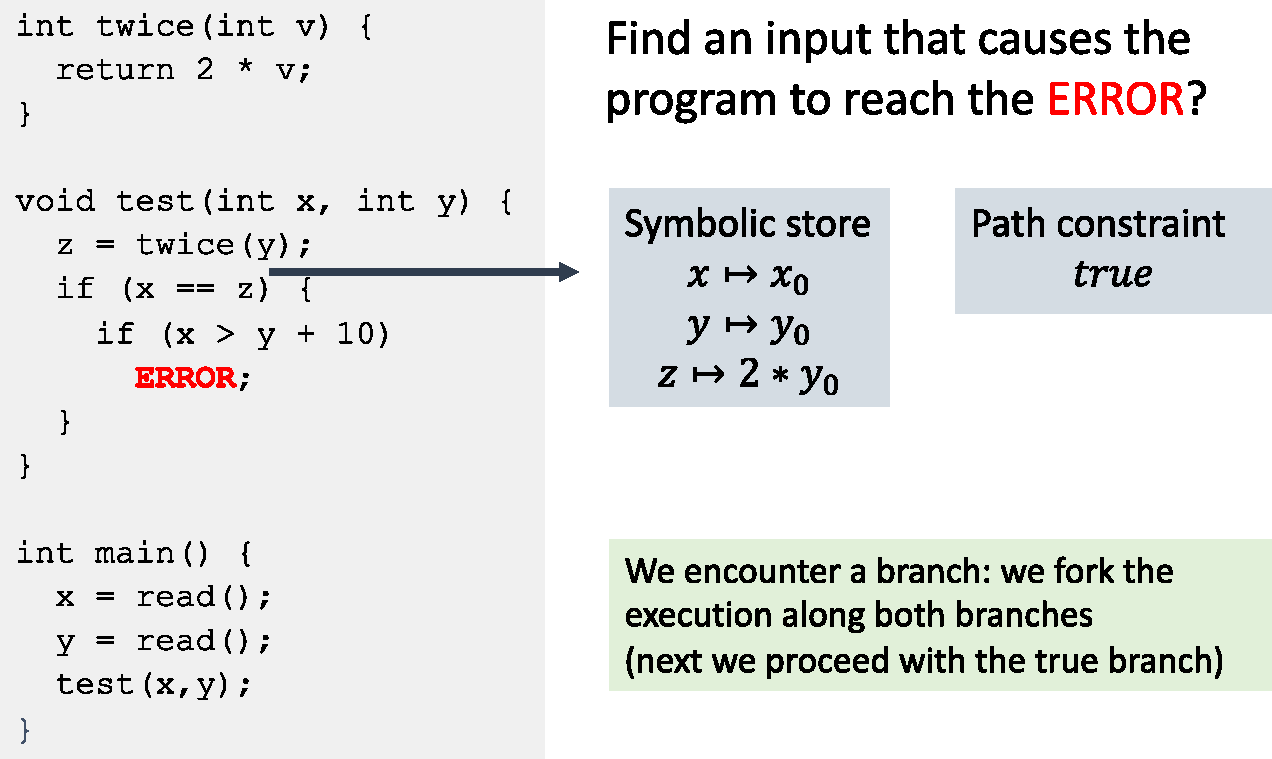
\includegraphics[width=\unitlength,page=1]{Figures/L4_symbolic_execution_example_2.pdf}}%
  \end{picture}%
\endgroup%
    
\end{minipage}
\begin{minipage}{0.5\linewidth}
    \centering      
    \def\svgwidth{\linewidth}
    %% Creator: Inkscape inkscape 0.92.4, www.inkscape.org
%% PDF/EPS/PS + LaTeX output extension by Johan Engelen, 2010
%% Accompanies image file 'L4_symbolic_execution_example.pdf' (pdf, eps, ps)
%%
%% To include the image in your LaTeX document, write
%%   \input{<filename>.pdf_tex}
%%  instead of
%%   \includegraphics{<filename>.pdf}
%% To scale the image, write
%%   \def\svgwidth{<desired width>}
%%   \input{<filename>.pdf_tex}
%%  instead of
%%   \includegraphics[width=<desired width>]{<filename>.pdf}
%%
%% Images with a different path to the parent latex file can
%% be accessed with the `import' package (which may need to be
%% installed) using
%%   \usepackage{import}
%% in the preamble, and then including the image with
%%   \import{<path to file>}{<filename>.pdf_tex}
%% Alternatively, one can specify
%%   \graphicspath{{<path to file>/}}
%% 
%% For more information, please see info/svg-inkscape on CTAN:
%%   http://tug.ctan.org/tex-archive/info/svg-inkscape
%%
\begingroup%
  \makeatletter%
  \providecommand\color[2][]{%
    \errmessage{(Inkscape) Color is used for the text in Inkscape, but the package 'color.sty' is not loaded}%
    \renewcommand\color[2][]{}%
  }%
  \providecommand\transparent[1]{%
    \errmessage{(Inkscape) Transparency is used (non-zero) for the text in Inkscape, but the package 'transparent.sty' is not loaded}%
    \renewcommand\transparent[1]{}%
  }%
  \providecommand\rotatebox[2]{#2}%
  \newcommand*\fsize{\dimexpr\f@size pt\relax}%
  \newcommand*\lineheight[1]{\fontsize{\fsize}{#1\fsize}\selectfont}%
  \ifx\svgwidth\undefined%
    \setlength{\unitlength}{608.67968942bp}%
    \ifx\svgscale\undefined%
      \relax%
    \else%
      \setlength{\unitlength}{\unitlength * \real{\svgscale}}%
    \fi%
  \else%
    \setlength{\unitlength}{\svgwidth}%
  \fi%
  \global\let\svgwidth\undefined%
  \global\let\svgscale\undefined%
  \makeatother%
  \begin{picture}(1,0.59823387)%
    \lineheight{1}%
    \setlength\tabcolsep{0pt}%
    \put(0,0){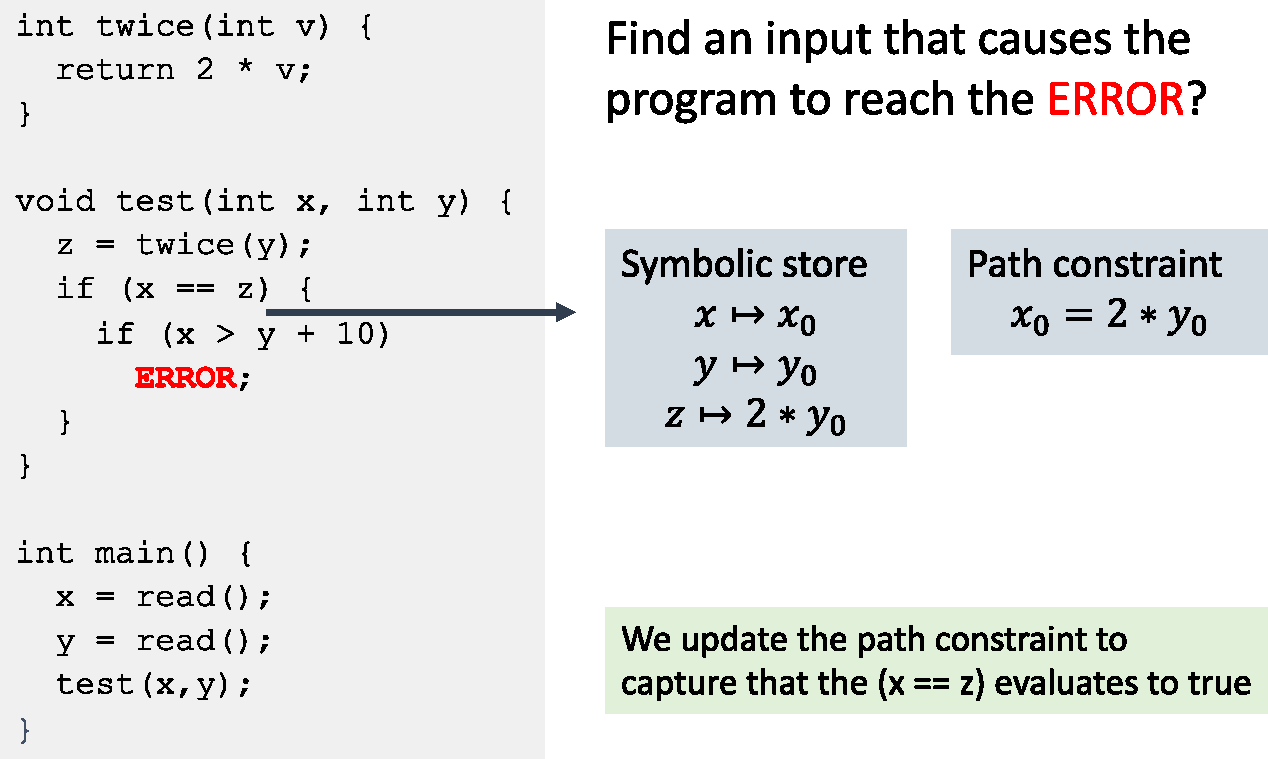
\includegraphics[width=\unitlength,page=1]{Figures/L4_symbolic_execution_example_3.pdf}}%
  \end{picture}%
\endgroup%
    
\end{minipage}
\begin{minipage}{0.5\linewidth}
    \centering      
    \def\svgwidth{\linewidth}
    %% Creator: Inkscape inkscape 0.92.4, www.inkscape.org
%% PDF/EPS/PS + LaTeX output extension by Johan Engelen, 2010
%% Accompanies image file 'L4_symbolic_execution_example_2.pdf' (pdf, eps, ps)
%%
%% To include the image in your LaTeX document, write
%%   \input{<filename>.pdf_tex}
%%  instead of
%%   \includegraphics{<filename>.pdf}
%% To scale the image, write
%%   \def\svgwidth{<desired width>}
%%   \input{<filename>.pdf_tex}
%%  instead of
%%   \includegraphics[width=<desired width>]{<filename>.pdf}
%%
%% Images with a different path to the parent latex file can
%% be accessed with the `import' package (which may need to be
%% installed) using
%%   \usepackage{import}
%% in the preamble, and then including the image with
%%   \import{<path to file>}{<filename>.pdf_tex}
%% Alternatively, one can specify
%%   \graphicspath{{<path to file>/}}
%% 
%% For more information, please see info/svg-inkscape on CTAN:
%%   http://tug.ctan.org/tex-archive/info/svg-inkscape
%%
\begingroup%
  \makeatletter%
  \providecommand\color[2][]{%
    \errmessage{(Inkscape) Color is used for the text in Inkscape, but the package 'color.sty' is not loaded}%
    \renewcommand\color[2][]{}%
  }%
  \providecommand\transparent[1]{%
    \errmessage{(Inkscape) Transparency is used (non-zero) for the text in Inkscape, but the package 'transparent.sty' is not loaded}%
    \renewcommand\transparent[1]{}%
  }%
  \providecommand\rotatebox[2]{#2}%
  \newcommand*\fsize{\dimexpr\f@size pt\relax}%
  \newcommand*\lineheight[1]{\fontsize{\fsize}{#1\fsize}\selectfont}%
  \ifx\svgwidth\undefined%
    \setlength{\unitlength}{638.22863001bp}%
    \ifx\svgscale\undefined%
      \relax%
    \else%
      \setlength{\unitlength}{\unitlength * \real{\svgscale}}%
    \fi%
  \else%
    \setlength{\unitlength}{\svgwidth}%
  \fi%
  \global\let\svgwidth\undefined%
  \global\let\svgscale\undefined%
  \makeatother%
  \begin{picture}(1,0.57336693)%
    \lineheight{1}%
    \setlength\tabcolsep{0pt}%
    \put(0,0){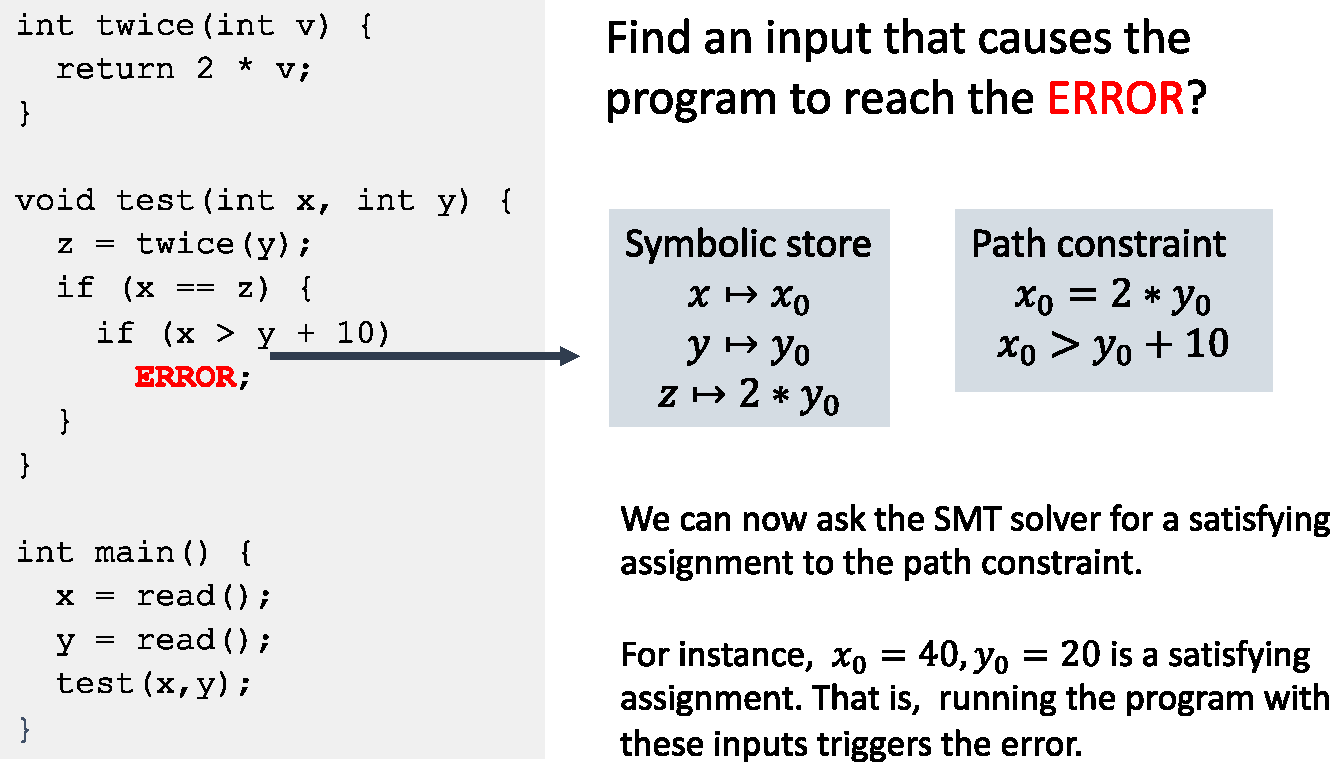
\includegraphics[width=\unitlength,page=1]{Figures/L4_symbolic_execution_example_4.pdf}}%
  \end{picture}%
\endgroup%
    
\end{minipage}

\paragraph{In Practice:}
\begin{itemize}
\item Many challenges:
\begin{itemize}
    \item Path explosion (exponential in number of branches)
    \item Constraint solving (e.g., non-linear and hash constraints)
\end{itemize}{}
\item Real-world symbolic execution fuzzers:
\begin{itemize}
    \item Stanford KLEE (http://klee.github.io/)
    \item NASA’s Java PathFinder (http://javapathfinder.sourceforge.net/)
    \item Microsoft SAGE
    \item UC Berkeley’s CUTE
\end{itemize}{}
\end{itemize}{}

\paragraph{Comparison:}
\begin{minipage}{0.5\linewidth}
    \centering      
    \def\svgwidth{\linewidth}
    %% Creator: Inkscape inkscape 0.92.4, www.inkscape.org
%% PDF/EPS/PS + LaTeX output extension by Johan Engelen, 2010
%% Accompanies image file 'L4_symbolic_execution_vs_Fuzzing.pdf' (pdf, eps, ps)
%%
%% To include the image in your LaTeX document, write
%%   \input{<filename>.pdf_tex}
%%  instead of
%%   \includegraphics{<filename>.pdf}
%% To scale the image, write
%%   \def\svgwidth{<desired width>}
%%   \input{<filename>.pdf_tex}
%%  instead of
%%   \includegraphics[width=<desired width>]{<filename>.pdf}
%%
%% Images with a different path to the parent latex file can
%% be accessed with the `import' package (which may need to be
%% installed) using
%%   \usepackage{import}
%% in the preamble, and then including the image with
%%   \import{<path to file>}{<filename>.pdf_tex}
%% Alternatively, one can specify
%%   \graphicspath{{<path to file>/}}
%% 
%% For more information, please see info/svg-inkscape on CTAN:
%%   http://tug.ctan.org/tex-archive/info/svg-inkscape
%%
\begingroup%
  \makeatletter%
  \providecommand\color[2][]{%
    \errmessage{(Inkscape) Color is used for the text in Inkscape, but the package 'color.sty' is not loaded}%
    \renewcommand\color[2][]{}%
  }%
  \providecommand\transparent[1]{%
    \errmessage{(Inkscape) Transparency is used (non-zero) for the text in Inkscape, but the package 'transparent.sty' is not loaded}%
    \renewcommand\transparent[1]{}%
  }%
  \providecommand\rotatebox[2]{#2}%
  \newcommand*\fsize{\dimexpr\f@size pt\relax}%
  \newcommand*\lineheight[1]{\fontsize{\fsize}{#1\fsize}\selectfont}%
  \ifx\svgwidth\undefined%
    \setlength{\unitlength}{578.74250757bp}%
    \ifx\svgscale\undefined%
      \relax%
    \else%
      \setlength{\unitlength}{\unitlength * \real{\svgscale}}%
    \fi%
  \else%
    \setlength{\unitlength}{\svgwidth}%
  \fi%
  \global\let\svgwidth\undefined%
  \global\let\svgscale\undefined%
  \makeatother%
  \begin{picture}(1,0.44964702)%
    \lineheight{1}%
    \setlength\tabcolsep{0pt}%
    \put(0,0){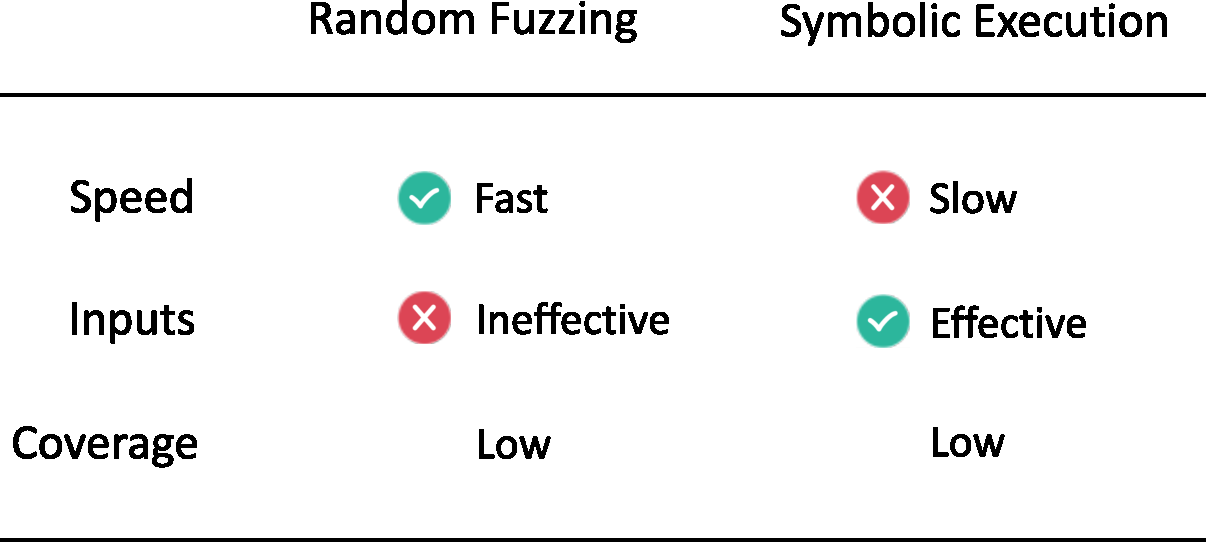
\includegraphics[width=\unitlength,page=1]{Figures/L4_symbolic_execution_vs_Fuzzing.pdf}}%
  \end{picture}%
\endgroup%
    
\end{minipage}

\subsection{Imitation Learning based Fuzzer ILF}

\begin{minipage}{0.75\linewidth}
    \centering      
    \def\svgwidth{\linewidth}
    %% Creator: Inkscape inkscape 0.92.4, www.inkscape.org
%% PDF/EPS/PS + LaTeX output extension by Johan Engelen, 2010
%% Accompanies image file 'L4_ILF.pdf' (pdf, eps, ps)
%%
%% To include the image in your LaTeX document, write
%%   \input{<filename>.pdf_tex}
%%  instead of
%%   \includegraphics{<filename>.pdf}
%% To scale the image, write
%%   \def\svgwidth{<desired width>}
%%   \input{<filename>.pdf_tex}
%%  instead of
%%   \includegraphics[width=<desired width>]{<filename>.pdf}
%%
%% Images with a different path to the parent latex file can
%% be accessed with the `import' package (which may need to be
%% installed) using
%%   \usepackage{import}
%% in the preamble, and then including the image with
%%   \import{<path to file>}{<filename>.pdf_tex}
%% Alternatively, one can specify
%%   \graphicspath{{<path to file>/}}
%% 
%% For more information, please see info/svg-inkscape on CTAN:
%%   http://tug.ctan.org/tex-archive/info/svg-inkscape
%%
\begingroup%
  \makeatletter%
  \providecommand\color[2][]{%
    \errmessage{(Inkscape) Color is used for the text in Inkscape, but the package 'color.sty' is not loaded}%
    \renewcommand\color[2][]{}%
  }%
  \providecommand\transparent[1]{%
    \errmessage{(Inkscape) Transparency is used (non-zero) for the text in Inkscape, but the package 'transparent.sty' is not loaded}%
    \renewcommand\transparent[1]{}%
  }%
  \providecommand\rotatebox[2]{#2}%
  \newcommand*\fsize{\dimexpr\f@size pt\relax}%
  \newcommand*\lineheight[1]{\fontsize{\fsize}{#1\fsize}\selectfont}%
  \ifx\svgwidth\undefined%
    \setlength{\unitlength}{634.3925416bp}%
    \ifx\svgscale\undefined%
      \relax%
    \else%
      \setlength{\unitlength}{\unitlength * \real{\svgscale}}%
    \fi%
  \else%
    \setlength{\unitlength}{\svgwidth}%
  \fi%
  \global\let\svgwidth\undefined%
  \global\let\svgscale\undefined%
  \makeatother%
  \begin{picture}(1,0.49303044)%
    \lineheight{1}%
    \setlength\tabcolsep{0pt}%
    \put(0,0){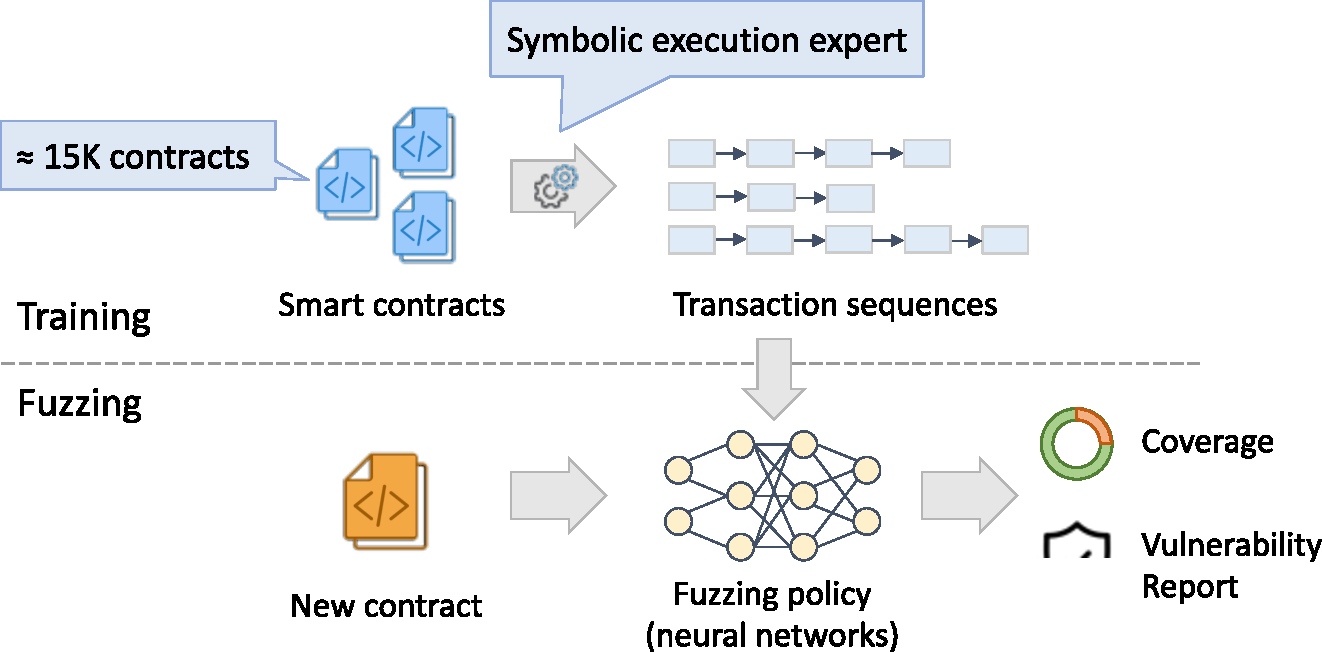
\includegraphics[width=\unitlength,page=1]{Figures/L4_ILF.pdf}}%
  \end{picture}%
\endgroup%
    
\end{minipage}
\paragraph{Fuzzing Policy:\newline}
\begin{minipage}{0.5\linewidth}
    \centering      
    \def\svgwidth{\linewidth}
    %% Creator: Inkscape inkscape 0.92.4, www.inkscape.org
%% PDF/EPS/PS + LaTeX output extension by Johan Engelen, 2010
%% Accompanies image file 'L4_ILF_fuzzing_policy.pdf' (pdf, eps, ps)
%%
%% To include the image in your LaTeX document, write
%%   \input{<filename>.pdf_tex}
%%  instead of
%%   \includegraphics{<filename>.pdf}
%% To scale the image, write
%%   \def\svgwidth{<desired width>}
%%   \input{<filename>.pdf_tex}
%%  instead of
%%   \includegraphics[width=<desired width>]{<filename>.pdf}
%%
%% Images with a different path to the parent latex file can
%% be accessed with the `import' package (which may need to be
%% installed) using
%%   \usepackage{import}
%% in the preamble, and then including the image with
%%   \import{<path to file>}{<filename>.pdf_tex}
%% Alternatively, one can specify
%%   \graphicspath{{<path to file>/}}
%% 
%% For more information, please see info/svg-inkscape on CTAN:
%%   http://tug.ctan.org/tex-archive/info/svg-inkscape
%%
\begingroup%
  \makeatletter%
  \providecommand\color[2][]{%
    \errmessage{(Inkscape) Color is used for the text in Inkscape, but the package 'color.sty' is not loaded}%
    \renewcommand\color[2][]{}%
  }%
  \providecommand\transparent[1]{%
    \errmessage{(Inkscape) Transparency is used (non-zero) for the text in Inkscape, but the package 'transparent.sty' is not loaded}%
    \renewcommand\transparent[1]{}%
  }%
  \providecommand\rotatebox[2]{#2}%
  \newcommand*\fsize{\dimexpr\f@size pt\relax}%
  \newcommand*\lineheight[1]{\fontsize{\fsize}{#1\fsize}\selectfont}%
  \ifx\svgwidth\undefined%
    \setlength{\unitlength}{651.1706543bp}%
    \ifx\svgscale\undefined%
      \relax%
    \else%
      \setlength{\unitlength}{\unitlength * \real{\svgscale}}%
    \fi%
  \else%
    \setlength{\unitlength}{\svgwidth}%
  \fi%
  \global\let\svgwidth\undefined%
  \global\let\svgscale\undefined%
  \makeatother%
  \begin{picture}(1,0.5471154)%
    \lineheight{1}%
    \setlength\tabcolsep{0pt}%
    \put(0,0){\includegraphics[width=\unitlength,page=1]{Figures/L4_ILF_fuzzing_policy.pdf}}%
  \end{picture}%
\endgroup%
    
\end{minipage}
\begin{minipage}{0.5\linewidth}
    \centering      
    \def\svgwidth{\linewidth}
    %% Creator: Inkscape inkscape 0.92.4, www.inkscape.org
%% PDF/EPS/PS + LaTeX output extension by Johan Engelen, 2010
%% Accompanies image file 'L4_ILF_fuzzing_policy.pdf' (pdf, eps, ps)
%%
%% To include the image in your LaTeX document, write
%%   \input{<filename>.pdf_tex}
%%  instead of
%%   \includegraphics{<filename>.pdf}
%% To scale the image, write
%%   \def\svgwidth{<desired width>}
%%   \input{<filename>.pdf_tex}
%%  instead of
%%   \includegraphics[width=<desired width>]{<filename>.pdf}
%%
%% Images with a different path to the parent latex file can
%% be accessed with the `import' package (which may need to be
%% installed) using
%%   \usepackage{import}
%% in the preamble, and then including the image with
%%   \import{<path to file>}{<filename>.pdf_tex}
%% Alternatively, one can specify
%%   \graphicspath{{<path to file>/}}
%% 
%% For more information, please see info/svg-inkscape on CTAN:
%%   http://tug.ctan.org/tex-archive/info/svg-inkscape
%%
\begingroup%
  \makeatletter%
  \providecommand\color[2][]{%
    \errmessage{(Inkscape) Color is used for the text in Inkscape, but the package 'color.sty' is not loaded}%
    \renewcommand\color[2][]{}%
  }%
  \providecommand\transparent[1]{%
    \errmessage{(Inkscape) Transparency is used (non-zero) for the text in Inkscape, but the package 'transparent.sty' is not loaded}%
    \renewcommand\transparent[1]{}%
  }%
  \providecommand\rotatebox[2]{#2}%
  \newcommand*\fsize{\dimexpr\f@size pt\relax}%
  \newcommand*\lineheight[1]{\fontsize{\fsize}{#1\fsize}\selectfont}%
  \ifx\svgwidth\undefined%
    \setlength{\unitlength}{634.74825641bp}%
    \ifx\svgscale\undefined%
      \relax%
    \else%
      \setlength{\unitlength}{\unitlength * \real{\svgscale}}%
    \fi%
  \else%
    \setlength{\unitlength}{\svgwidth}%
  \fi%
  \global\let\svgwidth\undefined%
  \global\let\svgscale\undefined%
  \makeatother%
  \begin{picture}(1,0.45047456)%
    \lineheight{1}%
    \setlength\tabcolsep{0pt}%
    \put(0,0){\includegraphics[width=\unitlength,page=1]{Figures/L4_ILF_fuzzing_policy_detail.pdf}}%
  \end{picture}%
\endgroup%
    
\end{minipage}
\begin{itemize}
    \item \textbf{GRU}: Gated Recurrent Units
    \begin{itemize}
        \item Can deal with variable length \textcolor{green}{sequential} inputs with hidden states
        \item A natural fit for our setting for handling \textcolor{green}{sequence of transactions}
    \end{itemize}{}
    \item Features of $f_{i-1}$ could be Coverage, opcodes, function name. (can be dynamic)
    \item Fully Connected Networks (\textbf{FCN}): Standard network with linear layers and ReLU activation functions
    \item Softmax: Normalizes function scores (output of \textbf{FCN$_{func}$}) to probability distrubtion
\end{itemize}{}
\textbf{Neural Network description}:

\begin{itemize}
    \item \textbf{Function: } FCN$_{func}$ + Softmax
    \item \textbf{Arguments: } GRU$_{int}$ + FCN$_{int}$. Initial distribution from expert. Challenges:
        \begin{itemize}
            \item Functions have a \textcolor{red}{variable} length of arguments
            \item Search space of arguments is \textcolor{red}{large} (e.g., integers of 256 bits)
        \end{itemize}{}
     \item \textbf{Senders: }  FCN$_{sender}$. Distribution over 5 predefined senders
      \item \textbf{Amount: }  FCN$_{amount}$. Distribution over 50 seed amount values from expert
\end{itemize}{}
\paragraph{Symbolic Execution Expert:}
\begin{itemize}
    \item Standard symbolic engines (breadth-first style):
    \begin{itemize}
        \item Operate on symbolic blockchain state and generate symbolictransactions.
        \item Only scale to limited depth (e.g. 3)
    \end{itemize}{}
    \item Our expert (depth-first style with revisits):
    \begin{itemize}
        \item Operates on concrete blockchain state and generate concrete transactions.
        \item Scales to large depth (e.g. 30) and large training set.
        \item Algorithm:
        \begin{enumerate}
            \item Start on initial blockchain state $b_{init}$
            \item Greedy search for transaction $t$ with highest coverage
            \item Execute transaction $t$ to get to next blockchain state $b_1$
            \item Revisit blockchain states $b_i$ and take different transactions to improve code coverage
            \item Repeat
        \end{enumerate}{}
 \end{itemize}
\end{itemize}{}
\paragraph{Miscellaneous}
\begin{itemize}
    \item \textbf{Training NN Fuzzing Policy: } Use Cross-Entropy Loss on inferred transactions and transactions by expert. aka standard supervised learning
    \item \textbf{ILF System: Reports the following:}
    \begin{itemize}
        \item Instruction coverage.
        \item Basic block coverage.
        \item Locking: The contract cannot send out but can receive ether.
        \item Leaking: An attacker can steal ether from the contract.
        \item Suicidal: An attacker can deconstruct the contract.
        \item Block Dependency: Ether transfer depends on block state variables.
        \item Unhandled Exception: Root call does not catch exceptions from child calls.
        \item Controlled Delegatecall: Transaction parameters explicitly flow into arguments of a delegatecall instruction.
    \end{itemize}{}
\end{itemize}{}
\section{Datalog and static analysis}

\subsection{Stratified Datalog}

\paragraph{Datalog:}
\begin{itemize}
    \item Declarative logic-programming language.
    \item Useful for expressing recursive queries.
    \item solid formal foundations.
    \item Used in:
    \begin{itemize}
        \item Security Analysis
        \item Network config analysis
        \item Access control
    \end{itemize}{}
\end{itemize}

\paragraph{Datalog atoms:} Datalog consists of a variety of atoms.

\begin{minipage}{0.5\linewidth}
    \centering      
    \def\svgwidth{\linewidth}
    %% Creator: Inkscape inkscape 0.92.4, www.inkscape.org
%% PDF/EPS/PS + LaTeX output extension by Johan Engelen, 2010
%% Accompanies image file 'L3_overflow_exploit.pdf' (pdf, eps, ps)
%%
%% To include the image in your LaTeX document, write
%%   \input{<filename>.pdf_tex}
%%  instead of
%%   \includegraphics{<filename>.pdf}
%% To scale the image, write
%%   \def\svgwidth{<desired width>}
%%   \input{<filename>.pdf_tex}
%%  instead of
%%   \includegraphics[width=<desired width>]{<filename>.pdf}
%%
%% Images with a different path to the parent latex file can
%% be accessed with the `import' package (which may need to be
%% installed) using
%%   \usepackage{import}
%% in the preamble, and then including the image with
%%   \import{<path to file>}{<filename>.pdf_tex}
%% Alternatively, one can specify
%%   \graphicspath{{<path to file>/}}
%% 
%% For more information, please see info/svg-inkscape on CTAN:
%%   http://tug.ctan.org/tex-archive/info/svg-inkscape
%%
\begingroup%
  \makeatletter%
  \providecommand\color[2][]{%
    \errmessage{(Inkscape) Color is used for the text in Inkscape, but the package 'color.sty' is not loaded}%
    \renewcommand\color[2][]{}%
  }%
  \providecommand\transparent[1]{%
    \errmessage{(Inkscape) Transparency is used (non-zero) for the text in Inkscape, but the package 'transparent.sty' is not loaded}%
    \renewcommand\transparent[1]{}%
  }%
  \providecommand\rotatebox[2]{#2}%
  \newcommand*\fsize{\dimexpr\f@size pt\relax}%
  \newcommand*\lineheight[1]{\fontsize{\fsize}{#1\fsize}\selectfont}%
  \ifx\svgwidth\undefined%
    \setlength{\unitlength}{720.00000454bp}%
    \ifx\svgscale\undefined%
      \relax%
    \else%
      \setlength{\unitlength}{\unitlength * \real{\svgscale}}%
    \fi%
  \else%
    \setlength{\unitlength}{\svgwidth}%
  \fi%
  \global\let\svgwidth\undefined%
  \global\let\svgscale\undefined%
  \makeatother%
  \begin{picture}(1,0.75)%
    \lineheight{1}%
    \setlength\tabcolsep{0pt}%
    \put(0,0){\includegraphics[width=\unitlength,page=1]{Figures/L5_datalog_atoms.pdf}}%
  \end{picture}%
\endgroup%
    
\end{minipage}  
\paragraph{Datalog programs:} 
\begin{itemize}
    \item A set of rules of the form $a \xleftarrow{} l_1,...,l_n$
    \item Where $l_1,...,l_n$ are literals of the form $a$ or $\neg a$
    \item A program is \textcolor{orange}{well-formed} if for any rule, all variables that appear in the head (left of arrow) also appear in the body (right of arrow). Plus the variables in the head are not allowed to be negated.
    \item Predicates are not allowed to by cyclic and appear in negative literals.
    \item A program is \textcolor{orange}{positive} if its rules do not contain negative literals.
    \item The semantics of a positive Datalog program P is the least-fixed point of it.
    \item For any positive Datalog program the consequence operator $T_P$ is \textcolor{orange}{monotone}, but not for programs with negation.
\end{itemize}{}

\paragraph{Consequence Operator $T_P / \jmath$:}
\begin{itemize}
    \item \textcolor{blue}{$T_p(I) = \{\sigma(a) | a \xleftarrow{} l_1,...,l_n \in P, \exists \sigma : \forall i \in [1,...,n]: I \vdash \sigma(l_i)\}$}
    \item[] where \textcolor{blue}{$I \vdash l_i$ if $l_i = a$ and $a \in I$}
    \item[] and \textcolor{blue}{$I \vdash l_i$ if $l_i = \neg a$ and $a \notin I$}
    \item Note that ($\jmath, \subseteq, \cup, \cap$) is a complete lattice.
    \item \textbf{Least-fixed point $lfp_{T_P}$} can be computed by iteratively applying the consequene operator until reaching a fixed-point.
\end{itemize}{}

\paragraph{Stratified Datalog programs:}
\begin{itemize}
    \item Same predicate rules in one stratum.
    \item Negated predicate defined in lower stratum.
    \item Positive predicates defined in curren or lower stratum.
    \item[$\xrightarrow{}$] For each stratum, compute the lfp that contains the lfp of the previous stratum.
\end{itemize}{}

\begin{minipage}{0.5\linewidth}
    \centering      
    \def\svgwidth{\linewidth}
    %% Creator: Inkscape 1.0 (4035a4fb49, 2020-05-01), www.inkscape.org
%% PDF/EPS/PS + LaTeX output extension by Johan Engelen, 2010
%% Accompanies image file 'L5_stratified_datalog.pdf' (pdf, eps, ps)
%%
%% To include the image in your LaTeX document, write
%%   \input{<filename>.pdf_tex}
%%  instead of
%%   \includegraphics{<filename>.pdf}
%% To scale the image, write
%%   \def\svgwidth{<desired width>}
%%   \input{<filename>.pdf_tex}
%%  instead of
%%   \includegraphics[width=<desired width>]{<filename>.pdf}
%%
%% Images with a different path to the parent latex file can
%% be accessed with the `import' package (which may need to be
%% installed) using
%%   \usepackage{import}
%% in the preamble, and then including the image with
%%   \import{<path to file>}{<filename>.pdf_tex}
%% Alternatively, one can specify
%%   \graphicspath{{<path to file>/}}
%% 
%% For more information, please see info/svg-inkscape on CTAN:
%%   http://tug.ctan.org/tex-archive/info/svg-inkscape
%%
\begingroup%
  \makeatletter%
  \providecommand\color[2][]{%
    \errmessage{(Inkscape) Color is used for the text in Inkscape, but the package 'color.sty' is not loaded}%
    \renewcommand\color[2][]{}%
  }%
  \providecommand\transparent[1]{%
    \errmessage{(Inkscape) Transparency is used (non-zero) for the text in Inkscape, but the package 'transparent.sty' is not loaded}%
    \renewcommand\transparent[1]{}%
  }%
  \providecommand\rotatebox[2]{#2}%
  \newcommand*\fsize{\dimexpr\f@size pt\relax}%
  \newcommand*\lineheight[1]{\fontsize{\fsize}{#1\fsize}\selectfont}%
  \ifx\svgwidth\undefined%
    \setlength{\unitlength}{720.00000454bp}%
    \ifx\svgscale\undefined%
      \relax%
    \else%
      \setlength{\unitlength}{\unitlength * \real{\svgscale}}%
    \fi%
  \else%
    \setlength{\unitlength}{\svgwidth}%
  \fi%
  \global\let\svgwidth\undefined%
  \global\let\svgscale\undefined%
  \makeatother%
  \begin{picture}(1,0.75)%
    \lineheight{1}%
    \setlength\tabcolsep{0pt}%
    \put(0,0){\includegraphics[width=\unitlength,page=1]{L5_stratified_datalog.pdf}}%
  \end{picture}%
\endgroup%    
\end{minipage} 

\subsection{Static analysis with Datalog}

\paragraph{Effective callback freedom EECF:} A contract is EECF if for any execution with external callbacks there exists an equivalent execution without external callbacks (which starts in the same state and reaches the same final state).
\begin{itemize}
    \item[$\xrightarrow{}$] In practice, developers enforce the following security property: \textcolor{red}{Do not perform any stat changes after calls to external contracts.}
\end{itemize}{}

\paragraph{Checking security properties:}
\begin{itemize}
    \item Usually we cannot automatically find all calls where a certain property does not hold, because smart contracts are Turing-complete.
    \item However, when contracts violate/satisfy a security property they often violate/satisfy a simpler property. (E.g. instead of EECF check if there are writes after call.value())
\end{itemize}{}

\paragraph{Securify: } v2.0

\begin{minipage}{0.9\linewidth}
    \centering      
    \def\svgwidth{\linewidth}
    %% Creator: Inkscape inkscape 0.92.4, www.inkscape.org
%% PDF/EPS/PS + LaTeX output extension by Johan Engelen, 2010
%% Accompanies image file 'L5_securify.pdf' (pdf, eps, ps)
%%
%% To include the image in your LaTeX document, write
%%   \input{<filename>.pdf_tex}
%%  instead of
%%   \includegraphics{<filename>.pdf}
%% To scale the image, write
%%   \def\svgwidth{<desired width>}
%%   \input{<filename>.pdf_tex}
%%  instead of
%%   \includegraphics[width=<desired width>]{<filename>.pdf}
%%
%% Images with a different path to the parent latex file can
%% be accessed with the `import' package (which may need to be
%% installed) using
%%   \usepackage{import}
%% in the preamble, and then including the image with
%%   \import{<path to file>}{<filename>.pdf_tex}
%% Alternatively, one can specify
%%   \graphicspath{{<path to file>/}}
%% 
%% For more information, please see info/svg-inkscape on CTAN:
%%   http://tug.ctan.org/tex-archive/info/svg-inkscape
%%
\begingroup%
  \makeatletter%
  \providecommand\color[2][]{%
    \errmessage{(Inkscape) Color is used for the text in Inkscape, but the package 'color.sty' is not loaded}%
    \renewcommand\color[2][]{}%
  }%
  \providecommand\transparent[1]{%
    \errmessage{(Inkscape) Transparency is used (non-zero) for the text in Inkscape, but the package 'transparent.sty' is not loaded}%
    \renewcommand\transparent[1]{}%
  }%
  \providecommand\rotatebox[2]{#2}%
  \newcommand*\fsize{\dimexpr\f@size pt\relax}%
  \newcommand*\lineheight[1]{\fontsize{\fsize}{#1\fsize}\selectfont}%
  \ifx\svgwidth\undefined%
    \setlength{\unitlength}{720.00000454bp}%
    \ifx\svgscale\undefined%
      \relax%
    \else%
      \setlength{\unitlength}{\unitlength * \real{\svgscale}}%
    \fi%
  \else%
    \setlength{\unitlength}{\svgwidth}%
  \fi%
  \global\let\svgwidth\undefined%
  \global\let\svgscale\undefined%
  \makeatother%
  \begin{picture}(1,0.75)%
    \lineheight{1}%
    \setlength\tabcolsep{0pt}%
    \put(0,0){\includegraphics[width=\unitlength,page=1]{Figures/L5_securify.pdf}}%
  \end{picture}%
\endgroup%
    
\end{minipage}

\begin{itemize}
    \item Securify compiles Solidity to IR (Intermediate Representation)
    \item Bytecode is too low-level and lacks semantic information (No function boundaries, no storage model)
    \item Source code (Solidity) is too rich/changes often. This leads to a complex analysis.
    \item \textbf{Basic blocks: }
    \begin{itemize}
        \item Sequence of statements without branching.
        \item Take Arguments
        \item All variables are in single static assignment (SSA) form.
        \item End with a transfer to next blocks
    \end{itemize}{}
    \item \textbf{Transfers:} Goto, Jumps, Branches. Args and return values passed to next block
    \item \textbf{Statements:} 
    \begin{itemize}
        \item Static Single Assignment (SSA): each variable is treated as a variable that stores the statement's result.
        \item Three address form: t0 = t1 op t2
    \end{itemize}{}
\end{itemize}{}

\paragraph{Securify: Inferring semantic facts}
\begin{itemize}
    \item Scalable inference of semantic facts using Datalog.
    \item IR $\xrightarrow{}$ Datalog input $\xrightarrow{}$ Datalog fixpoint.
\end{itemize}{}

\begin{minipage}{0.9\linewidth}
    \centering      
    \def\svgwidth{\linewidth}
    %% Creator: Inkscape inkscape 0.92.4, www.inkscape.org
%% PDF/EPS/PS + LaTeX output extension by Johan Engelen, 2010
%% Accompanies image file 'L5_semantic_facts.pdf' (pdf, eps, ps)
%%
%% To include the image in your LaTeX document, write
%%   \input{<filename>.pdf_tex}
%%  instead of
%%   \includegraphics{<filename>.pdf}
%% To scale the image, write
%%   \def\svgwidth{<desired width>}
%%   \input{<filename>.pdf_tex}
%%  instead of
%%   \includegraphics[width=<desired width>]{<filename>.pdf}
%%
%% Images with a different path to the parent latex file can
%% be accessed with the `import' package (which may need to be
%% installed) using
%%   \usepackage{import}
%% in the preamble, and then including the image with
%%   \import{<path to file>}{<filename>.pdf_tex}
%% Alternatively, one can specify
%%   \graphicspath{{<path to file>/}}
%% 
%% For more information, please see info/svg-inkscape on CTAN:
%%   http://tug.ctan.org/tex-archive/info/svg-inkscape
%%
\begingroup%
  \makeatletter%
  \providecommand\color[2][]{%
    \errmessage{(Inkscape) Color is used for the text in Inkscape, but the package 'color.sty' is not loaded}%
    \renewcommand\color[2][]{}%
  }%
  \providecommand\transparent[1]{%
    \errmessage{(Inkscape) Transparency is used (non-zero) for the text in Inkscape, but the package 'transparent.sty' is not loaded}%
    \renewcommand\transparent[1]{}%
  }%
  \providecommand\rotatebox[2]{#2}%
  \newcommand*\fsize{\dimexpr\f@size pt\relax}%
  \newcommand*\lineheight[1]{\fontsize{\fsize}{#1\fsize}\selectfont}%
  \ifx\svgwidth\undefined%
    \setlength{\unitlength}{600.3286781bp}%
    \ifx\svgscale\undefined%
      \relax%
    \else%
      \setlength{\unitlength}{\unitlength * \real{\svgscale}}%
    \fi%
  \else%
    \setlength{\unitlength}{\svgwidth}%
  \fi%
  \global\let\svgwidth\undefined%
  \global\let\svgscale\undefined%
  \makeatother%
  \begin{picture}(1,0.54994243)%
    \lineheight{1}%
    \setlength\tabcolsep{0pt}%
    \put(0,0){\includegraphics[width=\unitlength,page=1]{Figures/L5_semantic_facts.pdf}}%
  \end{picture}%
\endgroup%
    
\end{minipage}

\paragraph{Taint analysis:} 
\begin{itemize}
    \item Taint analysis is a popular method which consists to check which variables can be modified by the user input. All user input can be dangerous if they aren't properly checked.
    \item \textbf{Call-site sensitivity: }Function arguments are tainted as they are controlled by the user $\rightarrow$ \textcolor{blue}{\texttt{mayDepOn(arguments, tainted)}}
    \item Context tracks a bounded history of the most recent function calls (e.g. context = [func1, func2,...]). $\rightarrow$  \textcolor{blue}{\texttt{mayDepOn(context, variable, tainted)}}
\end{itemize}{}

\paragraph{Security patterns language:}
\begin{itemize}
    \item A security pattern is a logical formula over semantic predicates e.g:\\
    $\varphi = mayDepOn(X,Y) | mustFollow(L,L) | \neg \alpha | ...$
    \item We need to convert a Security property e.g. "No state changes after call instructions" to a suitable violation pattern for securify.
    \item Securify then creates a Security report, where all unsafe calls are reported as either violations or warnings.
\end{itemize}{}

\paragraph{Benefits of static analysis using Datalog:}
\begin{itemize}
    \item Declarative (concise spec of the analysis)
    \item Modular (can merge the rules of multiple analyses)
    \item Scalable (can leverage existing Datalog solvers)
\end{itemize}{}
\section{Functional specification}
\subsection{Introduction}
\paragraph{Smart contract vulnerabilities:}
\begin{itemize}
    \item Unexpected ether flows
    \item Unprivileged writes
    \item Use of unsafe inputs
    \item Reentrant method calls
    \item Transaction reordering
    \item Arithmetic overflows
\end{itemize}{}
\textbf{\color{blue}Unknown unknowns: }Some "cool" quote from Christoph Jentzsch: \textit{We believe more security audits or more tests would have made no difference. The main problem was that reviewers did not know what to look for.}\\
\textbf{The problem: \newline}
\begin{minipage}{0.5\linewidth}
    \centering      
    \def\svgwidth{\linewidth}
    %% Creator: Inkscape inkscape 0.92.4, www.inkscape.org
%% PDF/EPS/PS + LaTeX output extension by Johan Engelen, 2010
%% Accompanies image file 'L6_vulnerabilites_problems.pdf' (pdf, eps, ps)
%%
%% To include the image in your LaTeX document, write
%%   \input{<filename>.pdf_tex}
%%  instead of
%%   \includegraphics{<filename>.pdf}
%% To scale the image, write
%%   \def\svgwidth{<desired width>}
%%   \input{<filename>.pdf_tex}
%%  instead of
%%   \includegraphics[width=<desired width>]{<filename>.pdf}
%%
%% Images with a different path to the parent latex file can
%% be accessed with the `import' package (which may need to be
%% installed) using
%%   \usepackage{import}
%% in the preamble, and then including the image with
%%   \import{<path to file>}{<filename>.pdf_tex}
%% Alternatively, one can specify
%%   \graphicspath{{<path to file>/}}
%% 
%% For more information, please see info/svg-inkscape on CTAN:
%%   http://tug.ctan.org/tex-archive/info/svg-inkscape
%%
\begingroup%
  \makeatletter%
  \providecommand\color[2][]{%
    \errmessage{(Inkscape) Color is used for the text in Inkscape, but the package 'color.sty' is not loaded}%
    \renewcommand\color[2][]{}%
  }%
  \providecommand\transparent[1]{%
    \errmessage{(Inkscape) Transparency is used (non-zero) for the text in Inkscape, but the package 'transparent.sty' is not loaded}%
    \renewcommand\transparent[1]{}%
  }%
  \providecommand\rotatebox[2]{#2}%
  \newcommand*\fsize{\dimexpr\f@size pt\relax}%
  \newcommand*\lineheight[1]{\fontsize{\fsize}{#1\fsize}\selectfont}%
  \ifx\svgwidth\undefined%
    \setlength{\unitlength}{594.2851774bp}%
    \ifx\svgscale\undefined%
      \relax%
    \else%
      \setlength{\unitlength}{\unitlength * \real{\svgscale}}%
    \fi%
  \else%
    \setlength{\unitlength}{\svgwidth}%
  \fi%
  \global\let\svgwidth\undefined%
  \global\let\svgscale\undefined%
  \makeatother%
  \begin{picture}(1,0.26069923)%
    \lineheight{1}%
    \setlength\tabcolsep{0pt}%
    \put(0,0){\includegraphics[width=\unitlength,page=1]{Figures/L6_vulnerabilites_problems.pdf}}%
  \end{picture}%
\endgroup%
    
\end{minipage}
TODO WTF?
\subsection{Property Behaviors}
\paragraph{Definitions:}
\begin{itemize}
    \item \textbf{\textcolor{blue}{Execution}} = sequence of function calls
    \item \textbf{\textcolor{blue}{Behavior}} =  corresponding sequence of (message, state) pairs
    \item The set of possible  \textbf{\textcolor{blue}{execution trees}} is defined by the following grammar:\\
    Exec ::= Start$^{\infty}$ \quad Start ::= Call \quad Call::= Msg [ Cmd* ] \quad Cmd ::= Call | ...
    \item A \textbf{\textcolor{blue}{complete call}} of a bundle of contracts is a \textbf{\textcolor{blue}{subtree}} of a valid execution tree such that:
    \begin{enumerate}
        \item the root is a \textbf{\textcolor{blue}{call}} to the bundle
        \item \textbf{\textcolor{blue}{not nested}} in other such call
    \end{enumerate}{}
    \item Every  complete call of the bundle gives rise to an \textbf{\textcolor{blue}{observation of the bundle}} which records:
    \begin{enumerate}
        \item the \textbf{\textcolor{blue}{message}} used  to call the bundle
        \item the \textbf{\textcolor{blue}{bundle state}} right after the call
    \end{enumerate}{}
    \item A \textbf{\textcolor{blue}{property}} w.r.t. \textbf{\textcolor{blue}{the bundle}} is merely a set \textbf{$P$} of infinite observation sequences $\alpha$\\
    Examples:
    \begin{description}
        \item[$P_1$] = \{$\alpha$ : all investments in $\alpha$ get deposited to Escrow\}
        \item[$P_2$] = \{$\alpha$ : all withdrawals in $\alpha$ happen only after the Crowdsale was closed\}
        \item[$P_3$] = \{$\alpha$ : the Crowdsale is eventually closed in $\alpha$\}
    \end{description}{}
\end{itemize}{}
\paragraph{Safety vs Liveness\\}
\begin{multicols}{2}
 \textbf{Safety}  \\ \rule{\linewidth}{0.4pt} \\A safety property requires that something \textbf{\textcolor{blue}{bad never happen}}, e.g., a withdrawal  never happens before a closure. \\ \\ \textbf{Formally:\\}
$P$ is a \textbf{safety} property iff for all infinite $\alpha$
$$
\begin{array}{c}
\alpha \notin P \Leftrightarrow \exists \text { bad } \prec \alpha \forall \beta \in P: \text { bad } \not\prec \beta \\ \\
\textit { Safety } \sim \textit { correctness. }
\end{array}
$$
 \columnbreak 
 \\ \\ \textbf{Liveness}  \\ \rule{\linewidth}{0.4pt}  \\ A liveness property requires that something \textbf{\textcolor{blue}{good happens often enough}}, e.g., the crowdsale eventually closes. \\ \\
\textbf{Formally:}\\
$P$ is a \textbf{liveness} property iff for all finite $\alpha$
$$
\begin{array}{c}
\exists \beta: \alpha \beta \in P \\ \\
\textit {Liveness } \sim \textit {delivery}
\end{array}
$$
\end{multicols}
Examples:
\begin{description}
    \item[$P_1$] = \{$\alpha$ : all investments in $\alpha$ get deposited to Escrow\}
        \begin{enumerate}
            \item[--] \textcolor{blue}{Safety} (depends on English interpretation)
        \end{enumerate}
    \item[$P_2$] = \{$\alpha$ : all withdrawals in $\alpha$ happen only after the Crowdsale was closed\}
    \begin{enumerate}
            \item[--] \textcolor{blue}{Safety}
        \end{enumerate}
    \item[$P_3$] = \{$\alpha$ : the Crowdsale is eventually closed in $\alpha$\}
    \begin{enumerate}
            \item[--] \textcolor{blue}{Liveness}
        \end{enumerate}
\end{description}{}

\subsection{Linear Temporal Logic (LTL)}
\paragraph{Introduction}
Consider the property:
\{$\alpha$ : all withdrawals in $\alpha$ happen only after the Crowdsale was closed\}
\begin{enumerate}
   \item[--] Classical logic definition:\\
        $\varphi(\alpha) \equiv \forall t \in \mathbb{N}: \text { fun }[\alpha | t]]=\text { withdraw } \rightarrow \exists s \leqslant t: \text { fun }[\alpha | s]]=\text { close. }$
    \item[--] LTL definition \\
    $\varphi \equiv \square(\text { fun }=\text { withdraw } \rightarrow \text { Gfun }=\text { close })$
\end{enumerate}{}
\subsection{LTL Syntax}

\begin{multicols}{2}
 \textbf{Terms}  \\ \rule{\linewidth}{0.4pt} \begin{enumerate}
    \item[--] \textbf{\textcolor{blue}{Variables}} (a.k.a. flexible variables) fun, raised, goal, ...
    \item[--] \textbf{\textcolor{blue}{Constants}} (a.k.a. rigid variables) $u, v, w, \ldots, 0,1,2, \ldots$
    \item[--] Application of \textbf{\textcolor{blue}{function symbols}} raised \textbf{\textcolor{blue}{+}} goal, ...
 \end{enumerate}{}
 \\
 \columnbreak 
 \\ \\ \textbf{Formulas}  \\ \rule{\linewidth}{0.4pt}  
 \begin{enumerate}
    \item[--] Application of \textbf{\textcolor{purple}{relation symbols}} fun \textcolor{purple}{$=$} withdraw, raised \textcolor{purple}{$<=$} goal
    \item[--] Application of \textbf{\textcolor{purple}{logical connectives}} $\varphi \textcolor{purple}{\wedge} \psi, \varphi \textcolor{purple}{\vee} \psi, \varphi \textcolor{purple}{\rightarrow} \psi, \ldots$
    \item[--] Application of \textbf{\textcolor{purple}{temporal connectives}}
        $\textcolor{purple}{\square} \varphi, \textcolor{purple}{\diamond}\varphi, \textcolor{purple}{\blacksquare } \varphi, \textcolor{purple}{\diamondsuite} \varphi, \ldots$
 \end{enumerate}{}
 \end{multicols}
 
 TODO filled diamond\\
 filled square = \textbf{so far}
 \begin{minipage}{0.5\linewidth}
    \centering      
    \def\svgwidth{\linewidth}
    %% Creator: Inkscape inkscape 0.92.4, www.inkscape.org
%% PDF/EPS/PS + LaTeX output extension by Johan Engelen, 2010
%% Accompanies image file 'L6_LTL_semantics.pdf' (pdf, eps, ps)
%%
%% To include the image in your LaTeX document, write
%%   \input{<filename>.pdf_tex}
%%  instead of
%%   \includegraphics{<filename>.pdf}
%% To scale the image, write
%%   \def\svgwidth{<desired width>}
%%   \input{<filename>.pdf_tex}
%%  instead of
%%   \includegraphics[width=<desired width>]{<filename>.pdf}
%%
%% Images with a different path to the parent latex file can
%% be accessed with the `import' package (which may need to be
%% installed) using
%%   \usepackage{import}
%% in the preamble, and then including the image with
%%   \import{<path to file>}{<filename>.pdf_tex}
%% Alternatively, one can specify
%%   \graphicspath{{<path to file>/}}
%% 
%% For more information, please see info/svg-inkscape on CTAN:
%%   http://tug.ctan.org/tex-archive/info/svg-inkscape
%%
\begingroup%
  \makeatletter%
  \providecommand\color[2][]{%
    \errmessage{(Inkscape) Color is used for the text in Inkscape, but the package 'color.sty' is not loaded}%
    \renewcommand\color[2][]{}%
  }%
  \providecommand\transparent[1]{%
    \errmessage{(Inkscape) Transparency is used (non-zero) for the text in Inkscape, but the package 'transparent.sty' is not loaded}%
    \renewcommand\transparent[1]{}%
  }%
  \providecommand\rotatebox[2]{#2}%
  \newcommand*\fsize{\dimexpr\f@size pt\relax}%
  \newcommand*\lineheight[1]{\fontsize{\fsize}{#1\fsize}\selectfont}%
  \ifx\svgwidth\undefined%
    \setlength{\unitlength}{648.0000173bp}%
    \ifx\svgscale\undefined%
      \relax%
    \else%
      \setlength{\unitlength}{\unitlength * \real{\svgscale}}%
    \fi%
  \else%
    \setlength{\unitlength}{\svgwidth}%
  \fi%
  \global\let\svgwidth\undefined%
  \global\let\svgscale\undefined%
  \makeatother%
  \begin{picture}(1,0.59115184)%
    \lineheight{1}%
    \setlength\tabcolsep{0pt}%
    \put(0,0){\includegraphics[width=\unitlength,page=1]{Figures/L6_LTL_semantics.pdf}}%
  \end{picture}%
\endgroup%
    
\end{minipage}


\begin{multicols}{2}
 \textbf{Constants (a.k.a. rigid variables)}  \\ \rule{\linewidth}{0.4pt} \\
 A constant $u$ may vary in time only w.r.t. surrounding temporal connectives:
 \begin{description}
    \item[LTL:] $\quad \square \existsu:(cl=u) \wedge \otimes(c l=u+1)]$
    \item[Classical:] $ \forall t \in \mathbb{N}: \exists u: \operatorname{cl}[t]=u \wedge c\lfloor[t+1]=u+1$
\end{description}{}
 \columnbreak 
 \\ \\ \textbf{Variables (a.k.a. flexible variables)}  \\ \rule{\linewidth}{0.4pt}  \\
 A variable u may vary in time freely: 
 \begin{description}
     \item[LTL:] $\square \exists u:(\mathrm{cl}=u) \wedge \otimes(c l=u+1))$
     \item[Classical:] $\forall t \in \mathbb{N}: \exists u: \mathrm{cl}[t]=\mathrm{u}[t] \wedge \mathrm{cl}[t+1]=\mathrm{u}[t+1]+1$
 \end{description}{}
 \end{multicols}
 \paragraph{Duality: De Morgan’s laws}
 \begin{minipage}{0.5\linewidth}
    \centering      
    \def\svgwidth{\linewidth}
    %% Creator: Inkscape inkscape 0.92.4, www.inkscape.org
%% PDF/EPS/PS + LaTeX output extension by Johan Engelen, 2010
%% Accompanies image file 'L6_LTL_semantics.pdf' (pdf, eps, ps)
%%
%% To include the image in your LaTeX document, write
%%   \input{<filename>.pdf_tex}
%%  instead of
%%   \includegraphics{<filename>.pdf}
%% To scale the image, write
%%   \def\svgwidth{<desired width>}
%%   \input{<filename>.pdf_tex}
%%  instead of
%%   \includegraphics[width=<desired width>]{<filename>.pdf}
%%
%% Images with a different path to the parent latex file can
%% be accessed with the `import' package (which may need to be
%% installed) using
%%   \usepackage{import}
%% in the preamble, and then including the image with
%%   \import{<path to file>}{<filename>.pdf_tex}
%% Alternatively, one can specify
%%   \graphicspath{{<path to file>/}}
%% 
%% For more information, please see info/svg-inkscape on CTAN:
%%   http://tug.ctan.org/tex-archive/info/svg-inkscape
%%
\begingroup%
  \makeatletter%
  \providecommand\color[2][]{%
    \errmessage{(Inkscape) Color is used for the text in Inkscape, but the package 'color.sty' is not loaded}%
    \renewcommand\color[2][]{}%
  }%
  \providecommand\transparent[1]{%
    \errmessage{(Inkscape) Transparency is used (non-zero) for the text in Inkscape, but the package 'transparent.sty' is not loaded}%
    \renewcommand\transparent[1]{}%
  }%
  \providecommand\rotatebox[2]{#2}%
  \newcommand*\fsize{\dimexpr\f@size pt\relax}%
  \newcommand*\lineheight[1]{\fontsize{\fsize}{#1\fsize}\selectfont}%
  \ifx\svgwidth\undefined%
    \setlength{\unitlength}{487.35001211bp}%
    \ifx\svgscale\undefined%
      \relax%
    \else%
      \setlength{\unitlength}{\unitlength * \real{\svgscale}}%
    \fi%
  \else%
    \setlength{\unitlength}{\svgwidth}%
  \fi%
  \global\let\svgwidth\undefined%
  \global\let\svgscale\undefined%
  \makeatother%
  \begin{picture}(1,0.47466527)%
    \lineheight{1}%
    \setlength\tabcolsep{0pt}%
    \put(0,0){\includegraphics[width=\unitlength,page=1]{Figures/L6_LTL_demorgan.pdf}}%
  \end{picture}%
\endgroup%
    
\end{minipage}

\paragraph{Theorems:}
\begin{enumerate}
    \item[] If $\varphi$ is a non-temporal formula (no temporal connectives), $\square \varphi$ defines a safety property.
    \item[] If $\varphi$ be a past formula (no future connectives), $\square \varphi$ defines a safety property. Also known as \textbf{Canonical Safety}
\end{enumerate}{}

\section{Formal Verification}

\paragraph{Goal: } For a contract with a set of behaviours B and for a safety property P, prove that B $\subseteq$ P. Reduce this to assertion verification.

\paragraph{Verification Recipe: } Start with a bundle of contracts and a \textcolor{blue}{canonical safety} specification $\square\varphi$.
\begin{enumerate}
    \item Convert the bundle to a program $\Pi$ that generates all bundle behaviors B.
    \item Turn $\varphi$ to an \textcolor{blue}{assertion} by instrumenting $\Pi$ with variables tracking past values (now assertion = non-temporal formula).
    \item Use standard assertion verification techniques to verify $\varphi$.
\end{enumerate}

\paragraph{State Transition Systems: } The mathematical perspective of the verification.

\begin{minipage}{0.9\linewidth}
    \centering      
    \def\svgwidth{\linewidth}
    %% Creator: Inkscape inkscape 0.92.4, www.inkscape.org
%% PDF/EPS/PS + LaTeX output extension by Johan Engelen, 2010
%% Accompanies image file 'L7_sts.pdf' (pdf, eps, ps)
%%
%% To include the image in your LaTeX document, write
%%   \input{<filename>.pdf_tex}
%%  instead of
%%   \includegraphics{<filename>.pdf}
%% To scale the image, write
%%   \def\svgwidth{<desired width>}
%%   \input{<filename>.pdf_tex}
%%  instead of
%%   \includegraphics[width=<desired width>]{<filename>.pdf}
%%
%% Images with a different path to the parent latex file can
%% be accessed with the `import' package (which may need to be
%% installed) using
%%   \usepackage{import}
%% in the preamble, and then including the image with
%%   \import{<path to file>}{<filename>.pdf_tex}
%% Alternatively, one can specify
%%   \graphicspath{{<path to file>/}}
%% 
%% For more information, please see info/svg-inkscape on CTAN:
%%   http://tug.ctan.org/tex-archive/info/svg-inkscape
%%
\begingroup%
  \makeatletter%
  \providecommand\color[2][]{%
    \errmessage{(Inkscape) Color is used for the text in Inkscape, but the package 'color.sty' is not loaded}%
    \renewcommand\color[2][]{}%
  }%
  \providecommand\transparent[1]{%
    \errmessage{(Inkscape) Transparency is used (non-zero) for the text in Inkscape, but the package 'transparent.sty' is not loaded}%
    \renewcommand\transparent[1]{}%
  }%
  \providecommand\rotatebox[2]{#2}%
  \newcommand*\fsize{\dimexpr\f@size pt\relax}%
  \newcommand*\lineheight[1]{\fontsize{\fsize}{#1\fsize}\selectfont}%
  \ifx\svgwidth\undefined%
    \setlength{\unitlength}{422.08210691bp}%
    \ifx\svgscale\undefined%
      \relax%
    \else%
      \setlength{\unitlength}{\unitlength * \real{\svgscale}}%
    \fi%
  \else%
    \setlength{\unitlength}{\svgwidth}%
  \fi%
  \global\let\svgwidth\undefined%
  \global\let\svgscale\undefined%
  \makeatother%
  \begin{picture}(1,0.43223227)%
    \lineheight{1}%
    \setlength\tabcolsep{0pt}%
    \put(0,0){\includegraphics[width=\unitlength,page=1]{Figures/L7_sts.pdf}}%
  \end{picture}%
\endgroup%
    
\end{minipage}

\paragraph{Invariants: } 
\begin{itemize}
    \item {\textbf{Invariant:}} definition in image above. 
    \item proving invariants is too difficult, thats why we need inductive invariants.
    \item \textbf{Inductive Invariants:} An inductive invariant of a STS is a state property I such that \textcolor{blue}{$S_0 \subseteq I$ and $T[I] \subseteq I$}.
    \item \textbf{Theorem: } Every inductive invariant is an invariant.
\end{itemize}

\paragraph{How to prove inductiveness automatically?} 
\begin{itemize}
    \item Use the \textcolor{orange}{strongest postcondition} operator \textbf{sp} : Program x Assertion $\rightarrow$ Assertion.
\end{itemize}{}

\begin{minipage}{0.9\linewidth}
    \centering      
    \def\svgwidth{\linewidth}
    %% Creator: Inkscape inkscape 0.92.4, www.inkscape.org
%% PDF/EPS/PS + LaTeX output extension by Johan Engelen, 2010
%% Accompanies image file 'L7_strongest_postcondition.pdf' (pdf, eps, ps)
%%
%% To include the image in your LaTeX document, write
%%   \input{<filename>.pdf_tex}
%%  instead of
%%   \includegraphics{<filename>.pdf}
%% To scale the image, write
%%   \def\svgwidth{<desired width>}
%%   \input{<filename>.pdf_tex}
%%  instead of
%%   \includegraphics[width=<desired width>]{<filename>.pdf}
%%
%% Images with a different path to the parent latex file can
%% be accessed with the `import' package (which may need to be
%% installed) using
%%   \usepackage{import}
%% in the preamble, and then including the image with
%%   \import{<path to file>}{<filename>.pdf_tex}
%% Alternatively, one can specify
%%   \graphicspath{{<path to file>/}}
%% 
%% For more information, please see info/svg-inkscape on CTAN:
%%   http://tug.ctan.org/tex-archive/info/svg-inkscape
%%
\begingroup%
  \makeatletter%
  \providecommand\color[2][]{%
    \errmessage{(Inkscape) Color is used for the text in Inkscape, but the package 'color.sty' is not loaded}%
    \renewcommand\color[2][]{}%
  }%
  \providecommand\transparent[1]{%
    \errmessage{(Inkscape) Transparency is used (non-zero) for the text in Inkscape, but the package 'transparent.sty' is not loaded}%
    \renewcommand\transparent[1]{}%
  }%
  \providecommand\rotatebox[2]{#2}%
  \newcommand*\fsize{\dimexpr\f@size pt\relax}%
  \newcommand*\lineheight[1]{\fontsize{\fsize}{#1\fsize}\selectfont}%
  \ifx\svgwidth\undefined%
    \setlength{\unitlength}{403.18360772bp}%
    \ifx\svgscale\undefined%
      \relax%
    \else%
      \setlength{\unitlength}{\unitlength * \real{\svgscale}}%
    \fi%
  \else%
    \setlength{\unitlength}{\svgwidth}%
  \fi%
  \global\let\svgwidth\undefined%
  \global\let\svgscale\undefined%
  \makeatother%
  \begin{picture}(1,0.25458509)%
    \lineheight{1}%
    \setlength\tabcolsep{0pt}%
    \put(0,0){\includegraphics[width=\unitlength,page=1]{Figures/L7_strongest_postcondition.pdf}}%
  \end{picture}%
\endgroup%
    
\end{minipage}
\\

\begin{enumerate}
    \item 
    \begin{itemize}
        \item [a)] A state transition system ($S$, $S_0$, $T$) is given by two progtams \texttt{init} and \texttt{step}:
        \item[] \texttt{init; \textbf{while true} \{ step; \}}
        \item [b)] A candidate invariant / is given by a formula $\varphi$.
    \end{itemize}
    \item Use and automated theorem prover to prove the validity of the formulas:
    \begin{itemize}
        \item[a)] $\textbf{sp}$ (\texttt{init, true}) $\rightarrow$ $\varphi$; (encodes $S_0 \subseteq I$)
        \item[b)] $\textbf{sp}$ (\texttt{step,}) $\varphi \rightarrow \varphi$; (encodes $T[I] \subseteq I$)
    \end{itemize}{}
    \item[$\rightarrow$] \textcolor{blue}{Example of this process on slide 15.}
\end{enumerate}

\paragraph{Computing  $sp(\Pi,\varphi)$}\textbf{by symbolic execution:}

\begin{minipage}{0.9\linewidth}
    \centering      
    \def\svgwidth{\linewidth}
    %% Creator: Inkscape inkscape 0.92.4, www.inkscape.org
%% PDF/EPS/PS + LaTeX output extension by Johan Engelen, 2010
%% Accompanies image file 'L7_symbolic_exec.pdf' (pdf, eps, ps)
%%
%% To include the image in your LaTeX document, write
%%   \input{<filename>.pdf_tex}
%%  instead of
%%   \includegraphics{<filename>.pdf}
%% To scale the image, write
%%   \def\svgwidth{<desired width>}
%%   \input{<filename>.pdf_tex}
%%  instead of
%%   \includegraphics[width=<desired width>]{<filename>.pdf}
%%
%% Images with a different path to the parent latex file can
%% be accessed with the `import' package (which may need to be
%% installed) using
%%   \usepackage{import}
%% in the preamble, and then including the image with
%%   \import{<path to file>}{<filename>.pdf_tex}
%% Alternatively, one can specify
%%   \graphicspath{{<path to file>/}}
%% 
%% For more information, please see info/svg-inkscape on CTAN:
%%   http://tug.ctan.org/tex-archive/info/svg-inkscape
%%
\begingroup%
  \makeatletter%
  \providecommand\color[2][]{%
    \errmessage{(Inkscape) Color is used for the text in Inkscape, but the package 'color.sty' is not loaded}%
    \renewcommand\color[2][]{}%
  }%
  \providecommand\transparent[1]{%
    \errmessage{(Inkscape) Transparency is used (non-zero) for the text in Inkscape, but the package 'transparent.sty' is not loaded}%
    \renewcommand\transparent[1]{}%
  }%
  \providecommand\rotatebox[2]{#2}%
  \newcommand*\fsize{\dimexpr\f@size pt\relax}%
  \newcommand*\lineheight[1]{\fontsize{\fsize}{#1\fsize}\selectfont}%
  \ifx\svgwidth\undefined%
    \setlength{\unitlength}{414.1536245bp}%
    \ifx\svgscale\undefined%
      \relax%
    \else%
      \setlength{\unitlength}{\unitlength * \real{\svgscale}}%
    \fi%
  \else%
    \setlength{\unitlength}{\svgwidth}%
  \fi%
  \global\let\svgwidth\undefined%
  \global\let\svgscale\undefined%
  \makeatother%
  \begin{picture}(1,0.44668589)%
    \lineheight{1}%
    \setlength\tabcolsep{0pt}%
    \put(0,0){\includegraphics[width=\unitlength,page=1]{Figures/L7_symbolic_exec.pdf}}%
  \end{picture}%
\endgroup%
    
\end{minipage}

\begin{itemize}
    \item If $\Pi$ contains loops then, \#paths = $\infty$, requiring more sophisticated techniques.
    \item [$\rightarrow$] \textcolor{blue}{Example of this process on slide 18.}
\end{itemize}{}

\paragraph{How to prove non-inductive variants?}
\begin{itemize}
    \item Find an inductive strengthening $l$ manually: $l$ is inductive and $l \rightarrow \varphi$.
    \item and prove analogously the strengthening $l$ automatically.
\end{itemize}{}





\section{Network verification}
\subsection{Introduction}
\begin{itemize}
    \item Each router:\begin{itemize}
        \item Runs multiple routing protocols (e.g. OSPF, BGP, ISIS)
        \item Stores a configuration (parameters used by the protocols)
    \end{itemize}
    \item Forwarding table:\begin{itemize}
        \item Defines the next hop for any packet
        \item Collectively, the forwarding tables of all routers define the forwarding plane
    \end{itemize}
\end{itemize}
\begin{minipage}{\linewidth}
    \centering      
    \def\svgwidth{\linewidth}
    %% Creator: Inkscape 1.0 (4035a4fb49, 2020-05-01), www.inkscape.org
%% PDF/EPS/PS + LaTeX output extension by Johan Engelen, 2010
%% Accompanies image file 'L8_networkConfiguration.pdf' (pdf, eps, ps)
%%
%% To include the image in your LaTeX document, write
%%   \input{<filename>.pdf_tex}
%%  instead of
%%   \includegraphics{<filename>.pdf}
%% To scale the image, write
%%   \def\svgwidth{<desired width>}
%%   \input{<filename>.pdf_tex}
%%  instead of
%%   \includegraphics[width=<desired width>]{<filename>.pdf}
%%
%% Images with a different path to the parent latex file can
%% be accessed with the `import' package (which may need to be
%% installed) using
%%   \usepackage{import}
%% in the preamble, and then including the image with
%%   \import{<path to file>}{<filename>.pdf_tex}
%% Alternatively, one can specify
%%   \graphicspath{{<path to file>/}}
%% 
%% For more information, please see info/svg-inkscape on CTAN:
%%   http://tug.ctan.org/tex-archive/info/svg-inkscape
%%
\begingroup%
  \makeatletter%
  \providecommand\color[2][]{%
    \errmessage{(Inkscape) Color is used for the text in Inkscape, but the package 'color.sty' is not loaded}%
    \renewcommand\color[2][]{}%
  }%
  \providecommand\transparent[1]{%
    \errmessage{(Inkscape) Transparency is used (non-zero) for the text in Inkscape, but the package 'transparent.sty' is not loaded}%
    \renewcommand\transparent[1]{}%
  }%
  \providecommand\rotatebox[2]{#2}%
  \newcommand*\fsize{\dimexpr\f@size pt\relax}%
  \newcommand*\lineheight[1]{\fontsize{\fsize}{#1\fsize}\selectfont}%
  \ifx\svgwidth\undefined%
    \setlength{\unitlength}{720bp}%
    \ifx\svgscale\undefined%
      \relax%
    \else%
      \setlength{\unitlength}{\unitlength * \real{\svgscale}}%
    \fi%
  \else%
    \setlength{\unitlength}{\svgwidth}%
  \fi%
  \global\let\svgwidth\undefined%
  \global\let\svgscale\undefined%
  \makeatother%
  \begin{picture}(1,0.75)%
    \lineheight{1}%
    \setlength\tabcolsep{0pt}%
    \put(0,0){\includegraphics[width=\unitlength,page=1]{L8_networkConfiguration.pdf}}%
  \end{picture}%
\endgroup%
    
\end{minipage}
\paragraph{Why network configuration is hard:\newline}
We have multiple protocols (BGP, OSPF, IS-IS), each with their own low-level configurations (BGP-Policies, Link costs, Static routes). Also the protocols themselves interact with each other (Preferences like: static over OSPF; Dependencies: BGP relies OSPF)\newline
\paragraph{Example\newline}
\begin{minipage}{\linewidth}
    \centering      
    \def\svgwidth{\linewidth}
    %% Creator: Inkscape 1.0 (4035a4fb49, 2020-05-01), www.inkscape.org
%% PDF/EPS/PS + LaTeX output extension by Johan Engelen, 2010
%% Accompanies image file 'L8_networkConfiguration2.pdf' (pdf, eps, ps)
%%
%% To include the image in your LaTeX document, write
%%   \input{<filename>.pdf_tex}
%%  instead of
%%   \includegraphics{<filename>.pdf}
%% To scale the image, write
%%   \def\svgwidth{<desired width>}
%%   \input{<filename>.pdf_tex}
%%  instead of
%%   \includegraphics[width=<desired width>]{<filename>.pdf}
%%
%% Images with a different path to the parent latex file can
%% be accessed with the `import' package (which may need to be
%% installed) using
%%   \usepackage{import}
%% in the preamble, and then including the image with
%%   \import{<path to file>}{<filename>.pdf_tex}
%% Alternatively, one can specify
%%   \graphicspath{{<path to file>/}}
%% 
%% For more information, please see info/svg-inkscape on CTAN:
%%   http://tug.ctan.org/tex-archive/info/svg-inkscape
%%
\begingroup%
  \makeatletter%
  \providecommand\color[2][]{%
    \errmessage{(Inkscape) Color is used for the text in Inkscape, but the package 'color.sty' is not loaded}%
    \renewcommand\color[2][]{}%
  }%
  \providecommand\transparent[1]{%
    \errmessage{(Inkscape) Transparency is used (non-zero) for the text in Inkscape, but the package 'transparent.sty' is not loaded}%
    \renewcommand\transparent[1]{}%
  }%
  \providecommand\rotatebox[2]{#2}%
  \newcommand*\fsize{\dimexpr\f@size pt\relax}%
  \newcommand*\lineheight[1]{\fontsize{\fsize}{#1\fsize}\selectfont}%
  \ifx\svgwidth\undefined%
    \setlength{\unitlength}{720bp}%
    \ifx\svgscale\undefined%
      \relax%
    \else%
      \setlength{\unitlength}{\unitlength * \real{\svgscale}}%
    \fi%
  \else%
    \setlength{\unitlength}{\svgwidth}%
  \fi%
  \global\let\svgwidth\undefined%
  \global\let\svgscale\undefined%
  \makeatother%
  \begin{picture}(1,0.75)%
    \lineheight{1}%
    \setlength\tabcolsep{0pt}%
    \put(0,0){\includegraphics[width=\unitlength,page=1]{L8_networkConfiguration2.pdf}}%
  \end{picture}%
\endgroup%
    
\end{minipage}
\begin{minipage}{\linewidth}
    \centering      
    \def\svgwidth{\linewidth}
    %% Creator: Inkscape 1.0 (4035a4fb49, 2020-05-01), www.inkscape.org
%% PDF/EPS/PS + LaTeX output extension by Johan Engelen, 2010
%% Accompanies image file 'L8_ExampleExtended.pdf' (pdf, eps, ps)
%%
%% To include the image in your LaTeX document, write
%%   \input{<filename>.pdf_tex}
%%  instead of
%%   \includegraphics{<filename>.pdf}
%% To scale the image, write
%%   \def\svgwidth{<desired width>}
%%   \input{<filename>.pdf_tex}
%%  instead of
%%   \includegraphics[width=<desired width>]{<filename>.pdf}
%%
%% Images with a different path to the parent latex file can
%% be accessed with the `import' package (which may need to be
%% installed) using
%%   \usepackage{import}
%% in the preamble, and then including the image with
%%   \import{<path to file>}{<filename>.pdf_tex}
%% Alternatively, one can specify
%%   \graphicspath{{<path to file>/}}
%% 
%% For more information, please see info/svg-inkscape on CTAN:
%%   http://tug.ctan.org/tex-archive/info/svg-inkscape
%%
\begingroup%
  \makeatletter%
  \providecommand\color[2][]{%
    \errmessage{(Inkscape) Color is used for the text in Inkscape, but the package 'color.sty' is not loaded}%
    \renewcommand\color[2][]{}%
  }%
  \providecommand\transparent[1]{%
    \errmessage{(Inkscape) Transparency is used (non-zero) for the text in Inkscape, but the package 'transparent.sty' is not loaded}%
    \renewcommand\transparent[1]{}%
  }%
  \providecommand\rotatebox[2]{#2}%
  \newcommand*\fsize{\dimexpr\f@size pt\relax}%
  \newcommand*\lineheight[1]{\fontsize{\fsize}{#1\fsize}\selectfont}%
  \ifx\svgwidth\undefined%
    \setlength{\unitlength}{720bp}%
    \ifx\svgscale\undefined%
      \relax%
    \else%
      \setlength{\unitlength}{\unitlength * \real{\svgscale}}%
    \fi%
  \else%
    \setlength{\unitlength}{\svgwidth}%
  \fi%
  \global\let\svgwidth\undefined%
  \global\let\svgscale\undefined%
  \makeatother%
  \begin{picture}(1,0.75)%
    \lineheight{1}%
    \setlength\tabcolsep{0pt}%
    \put(0,0){\includegraphics[width=\unitlength,page=1]{L8_ExampleExtended.pdf}}%
  \end{picture}%
\endgroup%
    
\end{minipage}
\subsection{Analysis of Network Configurations via Datalog}
\begin{minipage}{\linewidth}
    \centering      
    \def\svgwidth{\linewidth}
    %% Creator: Inkscape 1.0 (4035a4fb49, 2020-05-01), www.inkscape.org
%% PDF/EPS/PS + LaTeX output extension by Johan Engelen, 2010
%% Accompanies image file 'L8_networkAnalysisWithDatalog.pdf' (pdf, eps, ps)
%%
%% To include the image in your LaTeX document, write
%%   \input{<filename>.pdf_tex}
%%  instead of
%%   \includegraphics{<filename>.pdf}
%% To scale the image, write
%%   \def\svgwidth{<desired width>}
%%   \input{<filename>.pdf_tex}
%%  instead of
%%   \includegraphics[width=<desired width>]{<filename>.pdf}
%%
%% Images with a different path to the parent latex file can
%% be accessed with the `import' package (which may need to be
%% installed) using
%%   \usepackage{import}
%% in the preamble, and then including the image with
%%   \import{<path to file>}{<filename>.pdf_tex}
%% Alternatively, one can specify
%%   \graphicspath{{<path to file>/}}
%% 
%% For more information, please see info/svg-inkscape on CTAN:
%%   http://tug.ctan.org/tex-archive/info/svg-inkscape
%%
\begingroup%
  \makeatletter%
  \providecommand\color[2][]{%
    \errmessage{(Inkscape) Color is used for the text in Inkscape, but the package 'color.sty' is not loaded}%
    \renewcommand\color[2][]{}%
  }%
  \providecommand\transparent[1]{%
    \errmessage{(Inkscape) Transparency is used (non-zero) for the text in Inkscape, but the package 'transparent.sty' is not loaded}%
    \renewcommand\transparent[1]{}%
  }%
  \providecommand\rotatebox[2]{#2}%
  \newcommand*\fsize{\dimexpr\f@size pt\relax}%
  \newcommand*\lineheight[1]{\fontsize{\fsize}{#1\fsize}\selectfont}%
  \ifx\svgwidth\undefined%
    \setlength{\unitlength}{599.71875bp}%
    \ifx\svgscale\undefined%
      \relax%
    \else%
      \setlength{\unitlength}{\unitlength * \real{\svgscale}}%
    \fi%
  \else%
    \setlength{\unitlength}{\svgwidth}%
  \fi%
  \global\let\svgwidth\undefined%
  \global\let\svgscale\undefined%
  \makeatother%
  \begin{picture}(1,0.54997134)%
    \lineheight{1}%
    \setlength\tabcolsep{0pt}%
    \put(0,0){\includegraphics[width=\unitlength,page=1]{L8_networkAnalysisWithDatalog.pdf}}%
  \end{picture}%
\endgroup%
    
\end{minipage}
\subsection{Batfish}
\begin{itemize}
\item Network configuration analyzer
 \item Available at http://www.batfish.org/
 \item Has found real bugs in real networks
 \item Three steps:
 \begin{enumerate}
    \item Parse configurations (to derive input facts)
    \item Compute forwarding plane (by computing a fixedpoint)
    \item Check for violations (by querying the fixed-point)
\end{enumerate}
\end{itemize}

\paragraph{Step 1: Parse configurations\newline}
\begin{minipage}{\linewidth}
    \centering      
    \def\svgwidth{\linewidth}
    %% Creator: Inkscape 1.0 (4035a4fb49, 2020-05-01), www.inkscape.org
%% PDF/EPS/PS + LaTeX output extension by Johan Engelen, 2010
%% Accompanies image file 'L8-configParsing.pdf' (pdf, eps, ps)
%%
%% To include the image in your LaTeX document, write
%%   \input{<filename>.pdf_tex}
%%  instead of
%%   \includegraphics{<filename>.pdf}
%% To scale the image, write
%%   \def\svgwidth{<desired width>}
%%   \input{<filename>.pdf_tex}
%%  instead of
%%   \includegraphics[width=<desired width>]{<filename>.pdf}
%%
%% Images with a different path to the parent latex file can
%% be accessed with the `import' package (which may need to be
%% installed) using
%%   \usepackage{import}
%% in the preamble, and then including the image with
%%   \import{<path to file>}{<filename>.pdf_tex}
%% Alternatively, one can specify
%%   \graphicspath{{<path to file>/}}
%% 
%% For more information, please see info/svg-inkscape on CTAN:
%%   http://tug.ctan.org/tex-archive/info/svg-inkscape
%%
\begingroup%
  \makeatletter%
  \providecommand\color[2][]{%
    \errmessage{(Inkscape) Color is used for the text in Inkscape, but the package 'color.sty' is not loaded}%
    \renewcommand\color[2][]{}%
  }%
  \providecommand\transparent[1]{%
    \errmessage{(Inkscape) Transparency is used (non-zero) for the text in Inkscape, but the package 'transparent.sty' is not loaded}%
    \renewcommand\transparent[1]{}%
  }%
  \providecommand\rotatebox[2]{#2}%
  \newcommand*\fsize{\dimexpr\f@size pt\relax}%
  \newcommand*\lineheight[1]{\fontsize{\fsize}{#1\fsize}\selectfont}%
  \ifx\svgwidth\undefined%
    \setlength{\unitlength}{619.48449707bp}%
    \ifx\svgscale\undefined%
      \relax%
    \else%
      \setlength{\unitlength}{\unitlength * \real{\svgscale}}%
    \fi%
  \else%
    \setlength{\unitlength}{\svgwidth}%
  \fi%
  \global\let\svgwidth\undefined%
  \global\let\svgscale\undefined%
  \makeatother%
  \begin{picture}(1,0.46173734)%
    \lineheight{1}%
    \setlength\tabcolsep{0pt}%
    \put(0,0){\includegraphics[width=\unitlength,page=1]{L8_configParsing.pdf}}%
  \end{picture}%
\endgroup%
    
\end{minipage}
\paragraph{Step 2: Compute forwarding plane}
\begin{itemize}
    \item Compute OSPF routes
    \begin{itemize}
    \item Input: OSPFLink(Router1, Router2, Cost)
    \item Wanted Output: BestOSPFRoute(Router, Network, NextHop)\newline
    \begin{minipage}{\linewidth}
    \centering      
    \def\svgwidth{\linewidth}
    %% Creator: Inkscape 1.0 (4035a4fb49, 2020-05-01), www.inkscape.org
%% PDF/EPS/PS + LaTeX output extension by Johan Engelen, 2010
%% Accompanies image file 'L8_step2_OSPF.pdf' (pdf, eps, ps)
%%
%% To include the image in your LaTeX document, write
%%   \input{<filename>.pdf_tex}
%%  instead of
%%   \includegraphics{<filename>.pdf}
%% To scale the image, write
%%   \def\svgwidth{<desired width>}
%%   \input{<filename>.pdf_tex}
%%  instead of
%%   \includegraphics[width=<desired width>]{<filename>.pdf}
%%
%% Images with a different path to the parent latex file can
%% be accessed with the `import' package (which may need to be
%% installed) using
%%   \usepackage{import}
%% in the preamble, and then including the image with
%%   \import{<path to file>}{<filename>.pdf_tex}
%% Alternatively, one can specify
%%   \graphicspath{{<path to file>/}}
%% 
%% For more information, please see info/svg-inkscape on CTAN:
%%   http://tug.ctan.org/tex-archive/info/svg-inkscape
%%
\begingroup%
  \makeatletter%
  \providecommand\color[2][]{%
    \errmessage{(Inkscape) Color is used for the text in Inkscape, but the package 'color.sty' is not loaded}%
    \renewcommand\color[2][]{}%
  }%
  \providecommand\transparent[1]{%
    \errmessage{(Inkscape) Transparency is used (non-zero) for the text in Inkscape, but the package 'transparent.sty' is not loaded}%
    \renewcommand\transparent[1]{}%
  }%
  \providecommand\rotatebox[2]{#2}%
  \newcommand*\fsize{\dimexpr\f@size pt\relax}%
  \newcommand*\lineheight[1]{\fontsize{\fsize}{#1\fsize}\selectfont}%
  \ifx\svgwidth\undefined%
    \setlength{\unitlength}{536.59008789bp}%
    \ifx\svgscale\undefined%
      \relax%
    \else%
      \setlength{\unitlength}{\unitlength * \real{\svgscale}}%
    \fi%
  \else%
    \setlength{\unitlength}{\svgwidth}%
  \fi%
  \global\let\svgwidth\undefined%
  \global\let\svgscale\undefined%
  \makeatother%
  \begin{picture}(1,0.59921234)%
    \lineheight{1}%
    \setlength\tabcolsep{0pt}%
    \put(0,0){\includegraphics[width=\unitlength,page=1]{L8_step2_OSPF.pdf}}%
  \end{picture}%
\endgroup%
    
\end{minipage}
\end{itemize}
    \item Compose protocols (by given preference)
    \begin{itemize}
        \item Inputs: 
        \begin{itemize}
            \item bestOSPFRoute(Router, Network, NextHop, Cost)
            \item static(Router, Network, NextHop)
            \item localPref(Router, Protocol, Preference)
        \end{itemize}
        \item Output: fwd(Router, Network, NextHop)\newline
        \begin{minipage}{\linewidth}
        \centering      
        \def\svgwidth{\linewidth}
        
        %% Creator: Inkscape 1.0 (4035a4fb49, 2020-05-01), www.inkscape.org
%% PDF/EPS/PS + LaTeX output extension by Johan Engelen, 2010
%% Accompanies image file 'L8_step2_OSPF.pdf' (pdf, eps, ps)
%%
%% To include the image in your LaTeX document, write
%%   \input{<filename>.pdf_tex}
%%  instead of
%%   \includegraphics{<filename>.pdf}
%% To scale the image, write
%%   \def\svgwidth{<desired width>}
%%   \input{<filename>.pdf_tex}
%%  instead of
%%   \includegraphics[width=<desired width>]{<filename>.pdf}
%%
%% Images with a different path to the parent latex file can
%% be accessed with the `import' package (which may need to be
%% installed) using
%%   \usepackage{import}
%% in the preamble, and then including the image with
%%   \import{<path to file>}{<filename>.pdf_tex}
%% Alternatively, one can specify
%%   \graphicspath{{<path to file>/}}
%% 
%% For more information, please see info/svg-inkscape on CTAN:
%%   http://tug.ctan.org/tex-archive/info/svg-inkscape
%%
\begingroup%
  \makeatletter%
  \providecommand\color[2][]{%
    \errmessage{(Inkscape) Color is used for the text in Inkscape, but the package 'color.sty' is not loaded}%
    \renewcommand\color[2][]{}%
  }%
  \providecommand\transparent[1]{%
    \errmessage{(Inkscape) Transparency is used (non-zero) for the text in Inkscape, but the package 'transparent.sty' is not loaded}%
    \renewcommand\transparent[1]{}%
  }%
  \providecommand\rotatebox[2]{#2}%
  \newcommand*\fsize{\dimexpr\f@size pt\relax}%
  \newcommand*\lineheight[1]{\fontsize{\fsize}{#1\fsize}\selectfont}%
  \ifx\svgwidth\undefined%
    \setlength{\unitlength}{600.79327393bp}%
    \ifx\svgscale\undefined%
      \relax%
    \else%
      \setlength{\unitlength}{\unitlength * \real{\svgscale}}%
    \fi%
  \else%
    \setlength{\unitlength}{\svgwidth}%
  \fi%
  \global\let\svgwidth\undefined%
  \global\let\svgscale\undefined%
  \makeatother%
  \begin{picture}(1,0.4467923)%
    \lineheight{1}%
    \setlength\tabcolsep{0pt}%
    \put(0,0){\includegraphics[width=\unitlength,page=1]{L8_step2_fwd.pdf}}%
  \end{picture}%
\endgroup%
   
        \end{minipage}
    \end{itemize}
\end{itemize}
\paragraph{Step 3: Analyze forwarding plane\newline}
For example: Detect Multi-path Inconsistencies with the following\newline
\vspace{0.5cm}
\begin{minipage}{0.5\linewidth}
        \centering      
        \def\svgwidth{\linewidth}
        %% Creator: Inkscape 1.0 (4035a4fb49, 2020-05-01), www.inkscape.org
%% PDF/EPS/PS + LaTeX output extension by Johan Engelen, 2010
%% Accompanies image file 'L8_multipath.pdf' (pdf, eps, ps)
%%
%% To include the image in your LaTeX document, write
%%   \input{<filename>.pdf_tex}
%%  instead of
%%   \includegraphics{<filename>.pdf}
%% To scale the image, write
%%   \def\svgwidth{<desired width>}
%%   \input{<filename>.pdf_tex}
%%  instead of
%%   \includegraphics[width=<desired width>]{<filename>.pdf}
%%
%% Images with a different path to the parent latex file can
%% be accessed with the `import' package (which may need to be
%% installed) using
%%   \usepackage{import}
%% in the preamble, and then including the image with
%%   \import{<path to file>}{<filename>.pdf_tex}
%% Alternatively, one can specify
%%   \graphicspath{{<path to file>/}}
%% 
%% For more information, please see info/svg-inkscape on CTAN:
%%   http://tug.ctan.org/tex-archive/info/svg-inkscape
%%
\begingroup%
  \makeatletter%
  \providecommand\color[2][]{%
    \errmessage{(Inkscape) Color is used for the text in Inkscape, but the package 'color.sty' is not loaded}%
    \renewcommand\color[2][]{}%
  }%
  \providecommand\transparent[1]{%
    \errmessage{(Inkscape) Transparency is used (non-zero) for the text in Inkscape, but the package 'transparent.sty' is not loaded}%
    \renewcommand\transparent[1]{}%
  }%
  \providecommand\rotatebox[2]{#2}%
  \newcommand*\fsize{\dimexpr\f@size pt\relax}%
  \newcommand*\lineheight[1]{\fontsize{\fsize}{#1\fsize}\selectfont}%
  \ifx\svgwidth\undefined%
    \setlength{\unitlength}{405.04266357bp}%
    \ifx\svgscale\undefined%
      \relax%
    \else%
      \setlength{\unitlength}{\unitlength * \real{\svgscale}}%
    \fi%
  \else%
    \setlength{\unitlength}{\svgwidth}%
  \fi%
  \global\let\svgwidth\undefined%
  \global\let\svgscale\undefined%
  \makeatother%
  \begin{picture}(1,0.96872564)%
    \lineheight{1}%
    \setlength\tabcolsep{0pt}%
    \put(0,0){\includegraphics[width=\unitlength,page=1]{L8_multipath.pdf}}%
  \end{picture}%
\endgroup%
   
\end{minipage}
\vspace{0.5cm}
\newline More properties:\newline
\begin{itemize}
    \item Paths: Packets for traffic class tc must follow the path \texttt{r1 -> ... -> r10}\newline \texttt{holds <- fwd(r1, tc, r2), ..., fwd(r9, tc, r10)}
    \item Traffic isolation: The paths for two distinct traffic classes \texttt{tc1} and \texttt{tc2} do not share links in the same direction\newline 
\texttt{holds <- $\forall$ R1, R2. fwd(R1, tc1, R2) => (!fwd(R1, tc2, R2))}
    \item Reachability: Router can reach a given traffic class
    \item Loop-freeness: The forwarding plane has no loops
\end{itemize}



\section{Network Synthesis}
\paragraph{Program Synthesis: } Learning a function from specifications (e.g. examples).
In this section we cover the synthesis of correct network configurations through incorporation of powerful SAT/SMT solvers. Two such network conficuration synthesisers are SyNET and NetComplete.

\subsection{SyNET}
\begin{minipage}{\linewidth}
    \centering      
    \def\svgwidth{\linewidth}
    %% Creator: Inkscape 1.0 (4035a4fb49, 2020-05-01), www.inkscape.org
%% PDF/EPS/PS + LaTeX output extension by Johan Engelen, 2010
%% Accompanies image file 'L9_SyNET.pdf' (pdf, eps, ps)
%%
%% To include the image in your LaTeX document, write
%%   \input{<filename>.pdf_tex}
%%  instead of
%%   \includegraphics{<filename>.pdf}
%% To scale the image, write
%%   \def\svgwidth{<desired width>}
%%   \input{<filename>.pdf_tex}
%%  instead of
%%   \includegraphics[width=<desired width>]{<filename>.pdf}
%%
%% Images with a different path to the parent latex file can
%% be accessed with the `import' package (which may need to be
%% installed) using
%%   \usepackage{import}
%% in the preamble, and then including the image with
%%   \import{<path to file>}{<filename>.pdf_tex}
%% Alternatively, one can specify
%%   \graphicspath{{<path to file>/}}
%% 
%% For more information, please see info/svg-inkscape on CTAN:
%%   http://tug.ctan.org/tex-archive/info/svg-inkscape
%%
\begingroup%
  \makeatletter%
  \providecommand\color[2][]{%
    \errmessage{(Inkscape) Color is used for the text in Inkscape, but the package 'color.sty' is not loaded}%
    \renewcommand\color[2][]{}%
  }%
  \providecommand\transparent[1]{%
    \errmessage{(Inkscape) Transparency is used (non-zero) for the text in Inkscape, but the package 'transparent.sty' is not loaded}%
    \renewcommand\transparent[1]{}%
  }%
  \providecommand\rotatebox[2]{#2}%
  \newcommand*\fsize{\dimexpr\f@size pt\relax}%
  \newcommand*\lineheight[1]{\fontsize{\fsize}{#1\fsize}\selectfont}%
  \ifx\svgwidth\undefined%
    \setlength{\unitlength}{720.00000454bp}%
    \ifx\svgscale\undefined%
      \relax%
    \else%
      \setlength{\unitlength}{\unitlength * \real{\svgscale}}%
    \fi%
  \else%
    \setlength{\unitlength}{\svgwidth}%
  \fi%
  \global\let\svgwidth\undefined%
  \global\let\svgscale\undefined%
  \makeatother%
  \begin{picture}(1,0.75)%
    \lineheight{1}%
    \setlength\tabcolsep{0pt}%
    \put(0,0){\includegraphics[width=\unitlength,page=1]{L9_SyNET.pdf}}%
  \end{picture}%
\endgroup%
    
\end{minipage}

\paragraph{Datalog rules vs SMT constraints: } Datalog rules are logical constraints that can be fed to an SMT solver.
\begin{itemize}
    \item constraints on datalog inputs (i.e. containing no derived datalog rules) can be converted directly to logical constraints.
    \item Derived datalog rules need a bit more work (unrolling) because the datalog derivation works different than the logical implication. 
\end{itemize}

\paragraph{Input synthesis for Datalog via SMT: }
\begin{enumerate}
    \item \textcolor{orange}{Encode Program P} into SMT constraints, which capture the fixed-point computed by P for a given input I.
    \item \textcolor{orange}{Encode query q} as assertions that must hold on the fixed-point.
    \item \textcolor{orange}{Get a model M} that satisfies the conjunction of the above constraints.
    \item \textcolor{orange}{Derive input I} from M by checking which atoms are true in M.
\end{enumerate}
\textcolor{red}{$\rightarrow$ But be careful: }In Datalog, given a rule $p \leftarrow q$, p is derived iff q is true. However in logic, the constraing $p \impliedby q$ is satisfied if p is true an q is false! Switch implication symbol to a if and only if symbol and unroll the datalog rule - make a formula for each time applying the consequence operator)\\
\textcolor{blue}{$\rightarrow$ What about negative queries?} Unrolling the Datalog rules works for positive queries beacause, by monotonicity of the consequence operator, any atom derived in a given step of the consequence operator is guaranteed to remain in the fixed point. For negative queries e.g. !path(1,3) we don't need to unroll, simply use the implication symbol.\\
\textcolor{blue}{$\rightarrow$ What about stratified Datalog?} Can be done by iteratively synthesizing an input for each stratum, starting from the highest stratum, going towards the lowest one. The iterative process may require backtracking if we end up with no possible solution.

\begin{minipage}{\linewidth}
    \centering      
    \def\svgwidth{\linewidth}
    %% Creator: Inkscape 1.0 (4035a4fb49, 2020-05-01), www.inkscape.org
%% PDF/EPS/PS + LaTeX output extension by Johan Engelen, 2010
%% Accompanies image file 'L9_InputSynthesis.pdf' (pdf, eps, ps)
%%
%% To include the image in your LaTeX document, write
%%   \input{<filename>.pdf_tex}
%%  instead of
%%   \includegraphics{<filename>.pdf}
%% To scale the image, write
%%   \def\svgwidth{<desired width>}
%%   \input{<filename>.pdf_tex}
%%  instead of
%%   \includegraphics[width=<desired width>]{<filename>.pdf}
%%
%% Images with a different path to the parent latex file can
%% be accessed with the `import' package (which may need to be
%% installed) using
%%   \usepackage{import}
%% in the preamble, and then including the image with
%%   \import{<path to file>}{<filename>.pdf_tex}
%% Alternatively, one can specify
%%   \graphicspath{{<path to file>/}}
%% 
%% For more information, please see info/svg-inkscape on CTAN:
%%   http://tug.ctan.org/tex-archive/info/svg-inkscape
%%
\begingroup%
  \makeatletter%
  \providecommand\color[2][]{%
    \errmessage{(Inkscape) Color is used for the text in Inkscape, but the package 'color.sty' is not loaded}%
    \renewcommand\color[2][]{}%
  }%
  \providecommand\transparent[1]{%
    \errmessage{(Inkscape) Transparency is used (non-zero) for the text in Inkscape, but the package 'transparent.sty' is not loaded}%
    \renewcommand\transparent[1]{}%
  }%
  \providecommand\rotatebox[2]{#2}%
  \newcommand*\fsize{\dimexpr\f@size pt\relax}%
  \newcommand*\lineheight[1]{\fontsize{\fsize}{#1\fsize}\selectfont}%
  \ifx\svgwidth\undefined%
    \setlength{\unitlength}{720.00000454bp}%
    \ifx\svgscale\undefined%
      \relax%
    \else%
      \setlength{\unitlength}{\unitlength * \real{\svgscale}}%
    \fi%
  \else%
    \setlength{\unitlength}{\svgwidth}%
  \fi%
  \global\let\svgwidth\undefined%
  \global\let\svgscale\undefined%
  \makeatother%
  \begin{picture}(1,0.75)%
    \lineheight{1}%
    \setlength\tabcolsep{0pt}%
    \put(0,0){\includegraphics[width=\unitlength,page=1]{L9_InputSynthesis.pdf}}%
  \end{picture}%
\endgroup%    
\end{minipage}

\paragraph{Challenges: }Key challenge is the scaling of synthesis for OSPF protocol (takes much more computation time)

\subsection{NetComplete}
\paragraph{Sketching: } A concept to express intent
\begin{itemize}
    \item Allow users to express insight by defining the hypothesis space and bias the search.
    \item Machine helps with low-level reasoning
\end{itemize}

\paragraph{Expressing Intent}Two ways to express intent and control hypothesis space:
\begin{itemize}
    \item \textcolor{orange}{Specifications: }Define what function you actually want:
    \begin{itemize}
        \item Assertions: \texttt{assert x > y;}
        \item Concrete Examples: \texttt{x = 5 or x = 6}
        \item Function Equivalence: \texttt{blockedMatMul(Mat a, Mat b) implements matMul}
    \end{itemize}
    \item \textcolor{orange}{Holes: }To be instantiated by the synthesizer. Fragment must come from a set defined by the user. Holes define the hypothesis space.\\
    
    \begin{minipage}{\linewidth}
    \centering      
    \def\svgwidth{\linewidth}
    %% Creator: Inkscape 1.0 (4035a4fb49, 2020-05-01), www.inkscape.org
%% PDF/EPS/PS + LaTeX output extension by Johan Engelen, 2010
%% Accompanies image file 'L9_Holes.pdf' (pdf, eps, ps)
%%
%% To include the image in your LaTeX document, write
%%   \input{<filename>.pdf_tex}
%%  instead of
%%   \includegraphics{<filename>.pdf}
%% To scale the image, write
%%   \def\svgwidth{<desired width>}
%%   \input{<filename>.pdf_tex}
%%  instead of
%%   \includegraphics[width=<desired width>]{<filename>.pdf}
%%
%% Images with a different path to the parent latex file can
%% be accessed with the `import' package (which may need to be
%% installed) using
%%   \usepackage{import}
%% in the preamble, and then including the image with
%%   \import{<path to file>}{<filename>.pdf_tex}
%% Alternatively, one can specify
%%   \graphicspath{{<path to file>/}}
%% 
%% For more information, please see info/svg-inkscape on CTAN:
%%   http://tug.ctan.org/tex-archive/info/svg-inkscape
%%
\begingroup%
  \makeatletter%
  \providecommand\color[2][]{%
    \errmessage{(Inkscape) Color is used for the text in Inkscape, but the package 'color.sty' is not loaded}%
    \renewcommand\color[2][]{}%
  }%
  \providecommand\transparent[1]{%
    \errmessage{(Inkscape) Transparency is used (non-zero) for the text in Inkscape, but the package 'transparent.sty' is not loaded}%
    \renewcommand\transparent[1]{}%
  }%
  \providecommand\rotatebox[2]{#2}%
  \newcommand*\fsize{\dimexpr\f@size pt\relax}%
  \newcommand*\lineheight[1]{\fontsize{\fsize}{#1\fsize}\selectfont}%
  \ifx\svgwidth\undefined%
    \setlength{\unitlength}{720.00000454bp}%
    \ifx\svgscale\undefined%
      \relax%
    \else%
      \setlength{\unitlength}{\unitlength * \real{\svgscale}}%
    \fi%
  \else%
    \setlength{\unitlength}{\svgwidth}%
  \fi%
  \global\let\svgwidth\undefined%
  \global\let\svgscale\undefined%
  \makeatother%
  \begin{picture}(1,0.75)%
    \lineheight{1}%
    \setlength\tabcolsep{0pt}%
    \put(0,0){\includegraphics[width=\unitlength,page=1]{L9_Holes.pdf}}%
  \end{picture}%
\endgroup%    
    \end{minipage}

\end{itemize}

\paragraph{Synthesizing functions: } Look at slides 49ff. (chume nöd ganz drus)
\begin{enumerate}
    \item Turn holes into special inputs of the function (Control inputs C)
    \item Constraining the set of controls. Constraints are collected into a predicate Q(x,c)
    \item Synthesize function: Learning reduces to constraint satisfaction
\end{enumerate}

\paragraph{Counter-example guided inductive synthesis (CEGIS): } CEGIS aims to find the right small set of examples S so that if we learn a function F satisfying S, then F is likely to be correct on all (potentially infinite set of) examples

\begin{minipage}{\linewidth}
    \centering      
    \def\svgwidth{\linewidth}
    %% Creator: Inkscape 1.0 (4035a4fb49, 2020-05-01), www.inkscape.org
%% PDF/EPS/PS + LaTeX output extension by Johan Engelen, 2010
%% Accompanies image file 'L9_CEGIS.pdf' (pdf, eps, ps)
%%
%% To include the image in your LaTeX document, write
%%   \input{<filename>.pdf_tex}
%%  instead of
%%   \includegraphics{<filename>.pdf}
%% To scale the image, write
%%   \def\svgwidth{<desired width>}
%%   \input{<filename>.pdf_tex}
%%  instead of
%%   \includegraphics[width=<desired width>]{<filename>.pdf}
%%
%% Images with a different path to the parent latex file can
%% be accessed with the `import' package (which may need to be
%% installed) using
%%   \usepackage{import}
%% in the preamble, and then including the image with
%%   \import{<path to file>}{<filename>.pdf_tex}
%% Alternatively, one can specify
%%   \graphicspath{{<path to file>/}}
%% 
%% For more information, please see info/svg-inkscape on CTAN:
%%   http://tug.ctan.org/tex-archive/info/svg-inkscape
%%
\begingroup%
  \makeatletter%
  \providecommand\color[2][]{%
    \errmessage{(Inkscape) Color is used for the text in Inkscape, but the package 'color.sty' is not loaded}%
    \renewcommand\color[2][]{}%
  }%
  \providecommand\transparent[1]{%
    \errmessage{(Inkscape) Transparency is used (non-zero) for the text in Inkscape, but the package 'transparent.sty' is not loaded}%
    \renewcommand\transparent[1]{}%
  }%
  \providecommand\rotatebox[2]{#2}%
  \newcommand*\fsize{\dimexpr\f@size pt\relax}%
  \newcommand*\lineheight[1]{\fontsize{\fsize}{#1\fsize}\selectfont}%
  \ifx\svgwidth\undefined%
    \setlength{\unitlength}{720.00000454bp}%
    \ifx\svgscale\undefined%
      \relax%
    \else%
      \setlength{\unitlength}{\unitlength * \real{\svgscale}}%
    \fi%
  \else%
    \setlength{\unitlength}{\svgwidth}%
  \fi%
  \global\let\svgwidth\undefined%
  \global\let\svgscale\undefined%
  \makeatother%
  \begin{picture}(1,0.75)%
    \lineheight{1}%
    \setlength\tabcolsep{0pt}%
    \put(0,0){\includegraphics[width=\unitlength,page=1]{L9_CEGIS.pdf}}%
  \end{picture}%
\endgroup%
    
    \end{minipage}

\paragraph{Efficient OSPF synthesis using CEGIS: } Define logical constraints that capture the OSPF requirements. Find cost assignment f such that requirements hold. Formula given to the solver.
\section{Big Code}
\paragraph{Big Code:} Create new software tools that leverage massive codebases to solve
problems beyond what is possible with traditional techniques. Usually the more specifications (understanding of how program code works) to standard models the better they get. The goal is to learn specifications automatically from large codebases.
\subsection{Example: Injection Attacks}
\paragraph{Tools to find Injection Attacks}
Use static taint analysis, but what about missing (not detected) sinks, sanitizers and sources? \\

\begin{minipage}{0.9\linewidth}
    \centering      
    \def\svgwidth{\columnwidth}
    %% Creator: Inkscape 1.0 (4035a4fb49, 2020-05-01), www.inkscape.org
%% PDF/EPS/PS + LaTeX output extension by Johan Engelen, 2010
%% Accompanies image file 'L10_Model.pdf' (pdf, eps, ps)
%%
%% To include the image in your LaTeX document, write
%%   \input{<filename>.pdf_tex}
%%  instead of
%%   \includegraphics{<filename>.pdf}
%% To scale the image, write
%%   \def\svgwidth{<desired width>}
%%   \input{<filename>.pdf_tex}
%%  instead of
%%   \includegraphics[width=<desired width>]{<filename>.pdf}
%%
%% Images with a different path to the parent latex file can
%% be accessed with the `import' package (which may need to be
%% installed) using
%%   \usepackage{import}
%% in the preamble, and then including the image with
%%   \import{<path to file>}{<filename>.pdf_tex}
%% Alternatively, one can specify
%%   \graphicspath{{<path to file>/}}
%% 
%% For more information, please see info/svg-inkscape on CTAN:
%%   http://tug.ctan.org/tex-archive/info/svg-inkscape
%%
\begingroup%
  \makeatletter%
  \providecommand\color[2][]{%
    \errmessage{(Inkscape) Color is used for the text in Inkscape, but the package 'color.sty' is not loaded}%
    \renewcommand\color[2][]{}%
  }%
  \providecommand\transparent[1]{%
    \errmessage{(Inkscape) Transparency is used (non-zero) for the text in Inkscape, but the package 'transparent.sty' is not loaded}%
    \renewcommand\transparent[1]{}%
  }%
  \providecommand\rotatebox[2]{#2}%
  \newcommand*\fsize{\dimexpr\f@size pt\relax}%
  \newcommand*\lineheight[1]{\fontsize{\fsize}{#1\fsize}\selectfont}%
  \ifx\svgwidth\undefined%
    \setlength{\unitlength}{720.00000454bp}%
    \ifx\svgscale\undefined%
      \relax%
    \else%
      \setlength{\unitlength}{\unitlength * \real{\svgscale}}%
    \fi%
  \else%
    \setlength{\unitlength}{\svgwidth}%
  \fi%
  \global\let\svgwidth\undefined%
  \global\let\svgscale\undefined%
  \makeatother%
  \begin{picture}(1,0.5625)%
    \lineheight{1}%
    \setlength\tabcolsep{0pt}%
    \put(0,0){\includegraphics[width=\unitlength,page=1]{L10_Model.pdf}}%
  \end{picture}%
\endgroup%    
\end{minipage}

\subsection{Pointer Analysis}
\paragraph{Problems with Pointer Analysis:}
\begin{itemize}
    \item Analysis of code for different libraries.
    \item Dynamic Runs (e.g. complex runtime behaviours of java.sql)
    \item Need knowledge how to analyze corner cases and libraries
\end{itemize}
\\
$\rightarrow$ Use ML for a scalable solution to pointer analysis!

\section{Exercises}

\paragraph{Revert vs. Require vs. Assert: }
\begin{itemize}
    \item Revert: Refund remaining Gas, Revert state and return a value, but does not take condition as argument.
    \item Require: Same as Revert but takes condition as argument.
    \item Assert: Burn all remaining Gas, Revert state.
\end{itemize}

\paragraph{Call vs. Send vs. Transfer}
\begin{itemize}
    \item Call: No error propagation but returns false, not safe against reentrancy. 
    \item Send: No error propagation but returns false if there is an error. Only gas for one single event.
    \item Transfer: Error propagation, Only gas for single event
\end{itemize}
\end{multicols*}
\end{document}